\documentclass[aspectratio=169,12pt]{beamer}
\usepackage[utf8]{inputenc}
\usepackage[T5]{fontenc}
\usepackage[vietnamese]{babel}
\usepackage{lmodern}
\usepackage{graphicx}
\usepackage{booktabs}
\usepackage{tabularx}
\usepackage{multicol}
\usepackage{tikz}
\usepackage{xcolor}

\usetheme{Madrid}
\usefonttheme{professionalfonts}

% --- Custom Colors & Settings ---
\definecolor{UBrandBlue}{RGB}{0, 71, 155}
\definecolor{UBrandGold}{RGB}{255, 184, 28}
\setbeamercolor{palette primary}{bg=UBrandBlue,fg=white}
\setbeamercolor{palette secondary}{bg=UBrandGold,fg=black}
\setbeamercolor{palette tertiary}{bg=UBrandBlue!80!black,fg=white}
\setbeamercolor{title}{bg=UBrandBlue,fg=white}
\setbeamercolor{item}{fg=UBrandBlue}


\title[Thực hành - Chương 07]{Khám phá Dữ liệu}
\subtitle{Analysis: Data Exploration}
\author[Giảng viên]{Trí tuệ Nhân tạo cho Kế toán (AI in Accounting)}
\institute[Đại học]{Khoa Kế toán - Kiểm toán}
\date{Bài giảng Thực hành 07}

\begin{document}

\begin{frame}
    \titlepage
\end{frame}

\begin{frame}{Góc nhìn Chuyên gia (Professional Insight)}
\begin{itemize}
    \item \textbf{Tầm quan trọng:} Khám phá dữ liệu là bước đầu tiên để "làm quen" với dữ liệu. Kế toán viên cần hiểu rõ dữ liệu của mình trước khi đưa ra bất kỳ kết luận hay báo cáo nào.
    \item \textbf{Trực giác Kế toán:} Kết hợp kinh nghiệm thực tiễn và kỹ năng phân tích để phát hiện ra các điểm bất thường, xu hướng hoặc insight tiềm ẩn.
    \item \textbf{Kể chuyện bằng dữ liệu (Data Storytelling):} Một biểu đồ trực quan tốt có giá trị hơn hàng ngàn con số trong bảng tính phức tạp.
\end{itemize}
\end{frame}

\begin{frame}{Lộ trình Chương (Chapter Roadmap)}
\begin{itemize}
    \item \textbf{LO 7.1:} Quy trình Khám phá Dữ liệu.
    \item \textbf{LO 7.2:} Khám phá Mối quan hệ Nền tảng qua 8 Mẫu Trực quan hóa.
    \item \textbf{LO 7.3:} Khám phá Dữ liệu bằng cách Tích hợp Mối quan hệ (Dashboards).
\end{itemize}
\end{frame}

\begin{frame}{7.1 Khám phá Dữ liệu (Data Exploration) là gì?}
\begin{itemize}
    \item \textbf{Định nghĩa:} Là quá trình phân tích dữ liệu ban đầu bằng các công cụ trực quan và thống kê để hiểu rõ đặc điểm, phát hiện xu hướng và kiểm tra các giả định.
    \item \textbf{Sự khác biệt:}
    \begin{itemize}
        \item \textbf{Khám phá (Exploration):} Tự do tìm kiếm insight (cho chính bạn).
        \item \textbf{Diễn giải (Interpretation):} Hiểu ý nghĩa của insight.
        \item \textbf{Báo cáo (Reporting):} Trình bày insight cho người khác (Management/Stakeholders).
    \end{itemize}
\end{itemize}
\end{frame}

\begin{frame}{ILLUSTRATION 7.1}

    \begin{figure}[h]
        \centering
        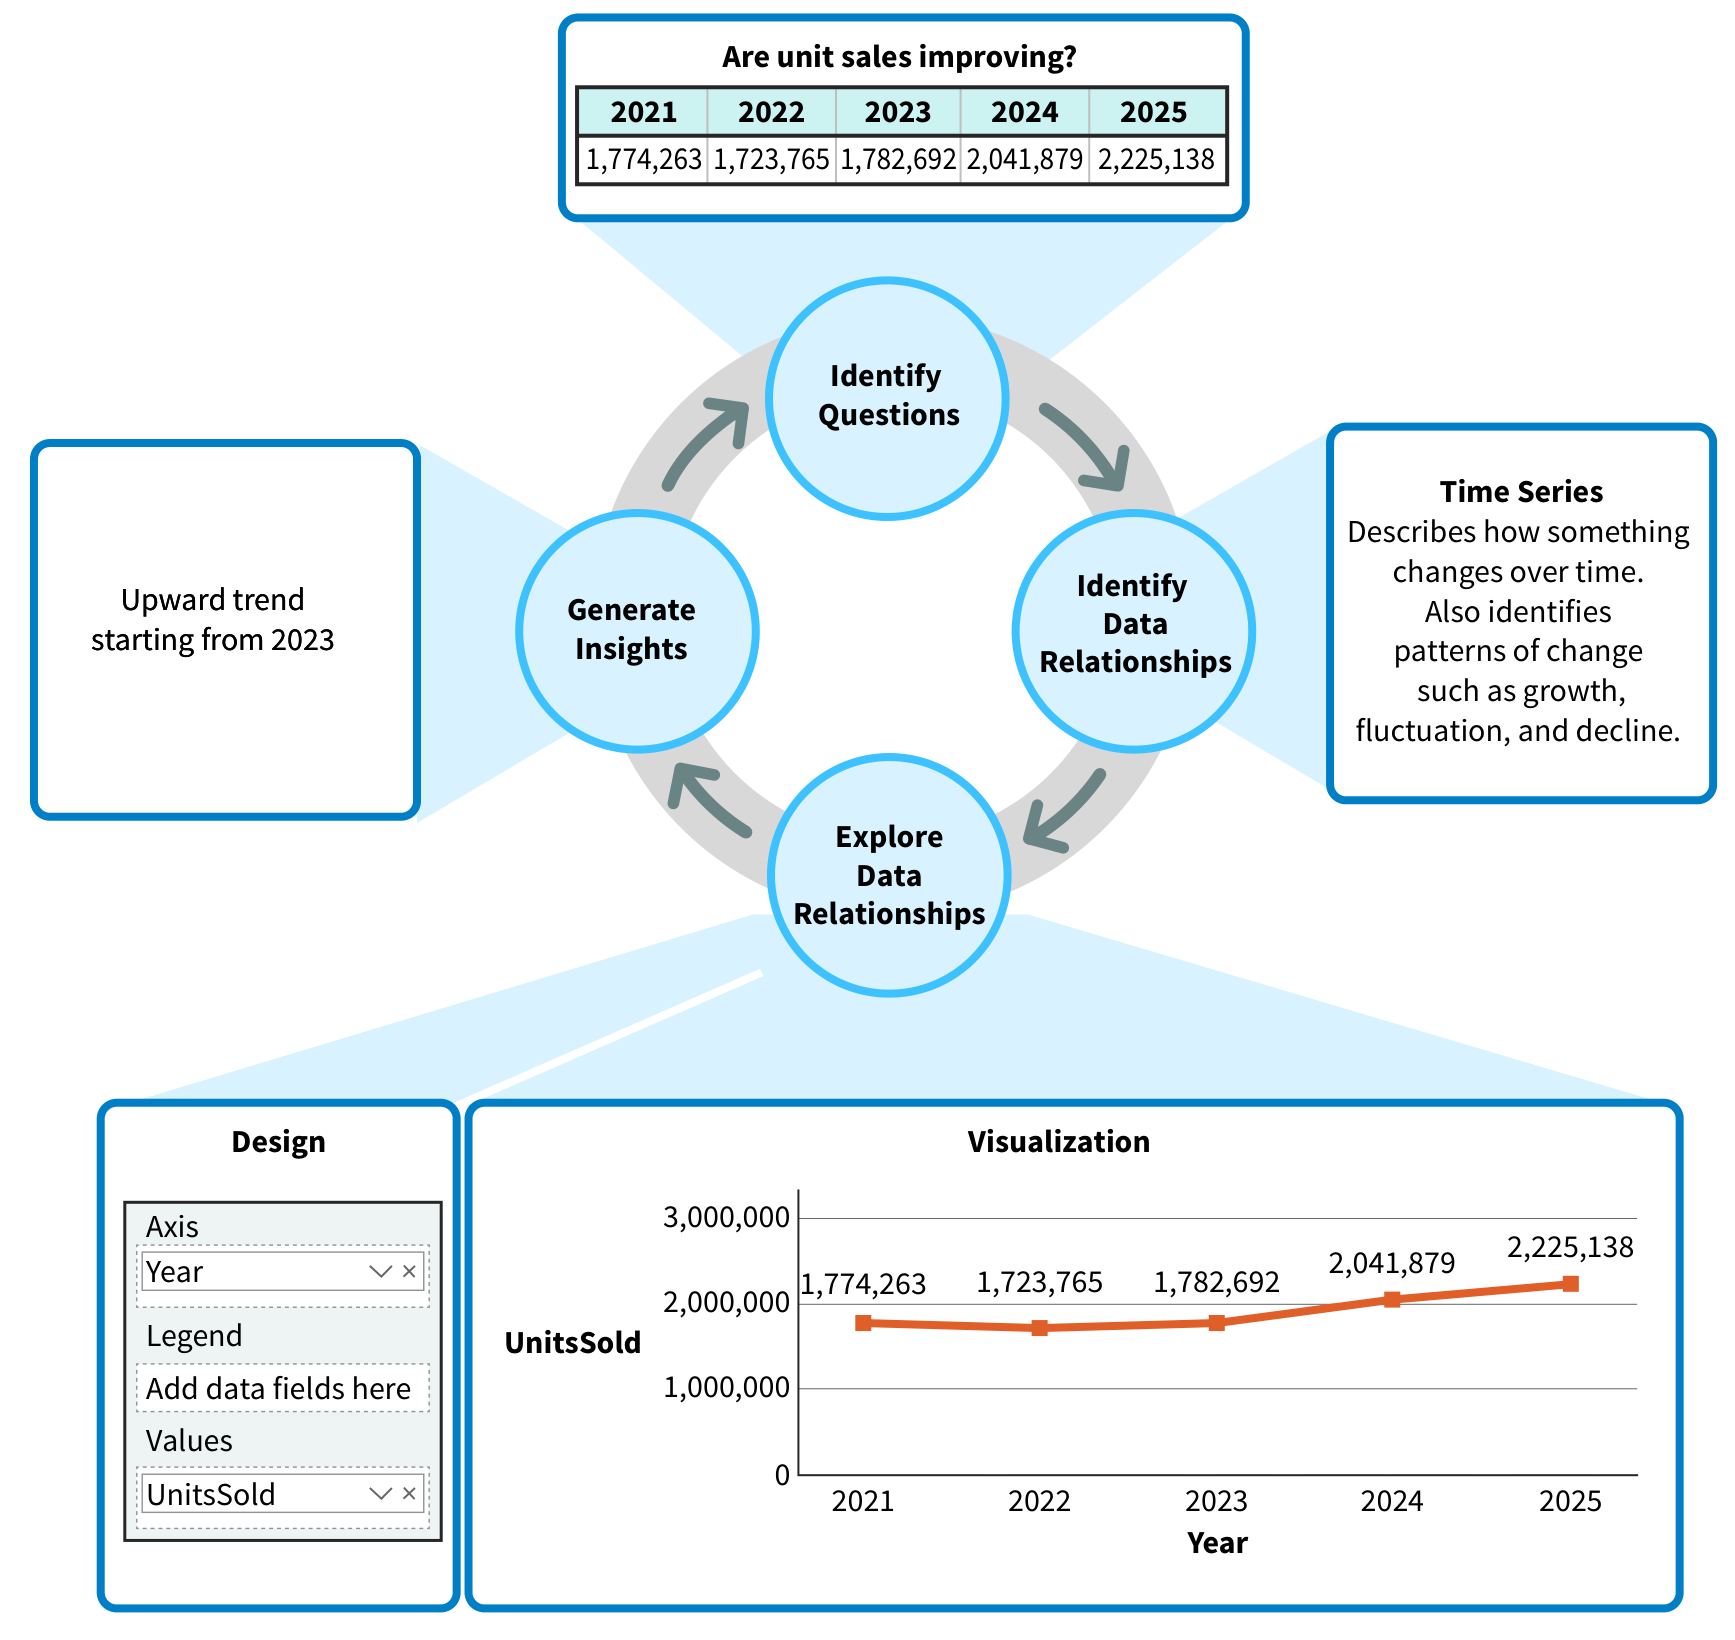
\includegraphics[width=0.95\textwidth,height=0.75\textheight,keepaspectratio]{../textbookForPractice/Figures/Ch_07/ILLUSTRATION 7.1.png}
    \end{figure}
\end{frame}

\begin{frame}{ILLUSTRATION 7.2}

    \begin{figure}[h]
        \centering
        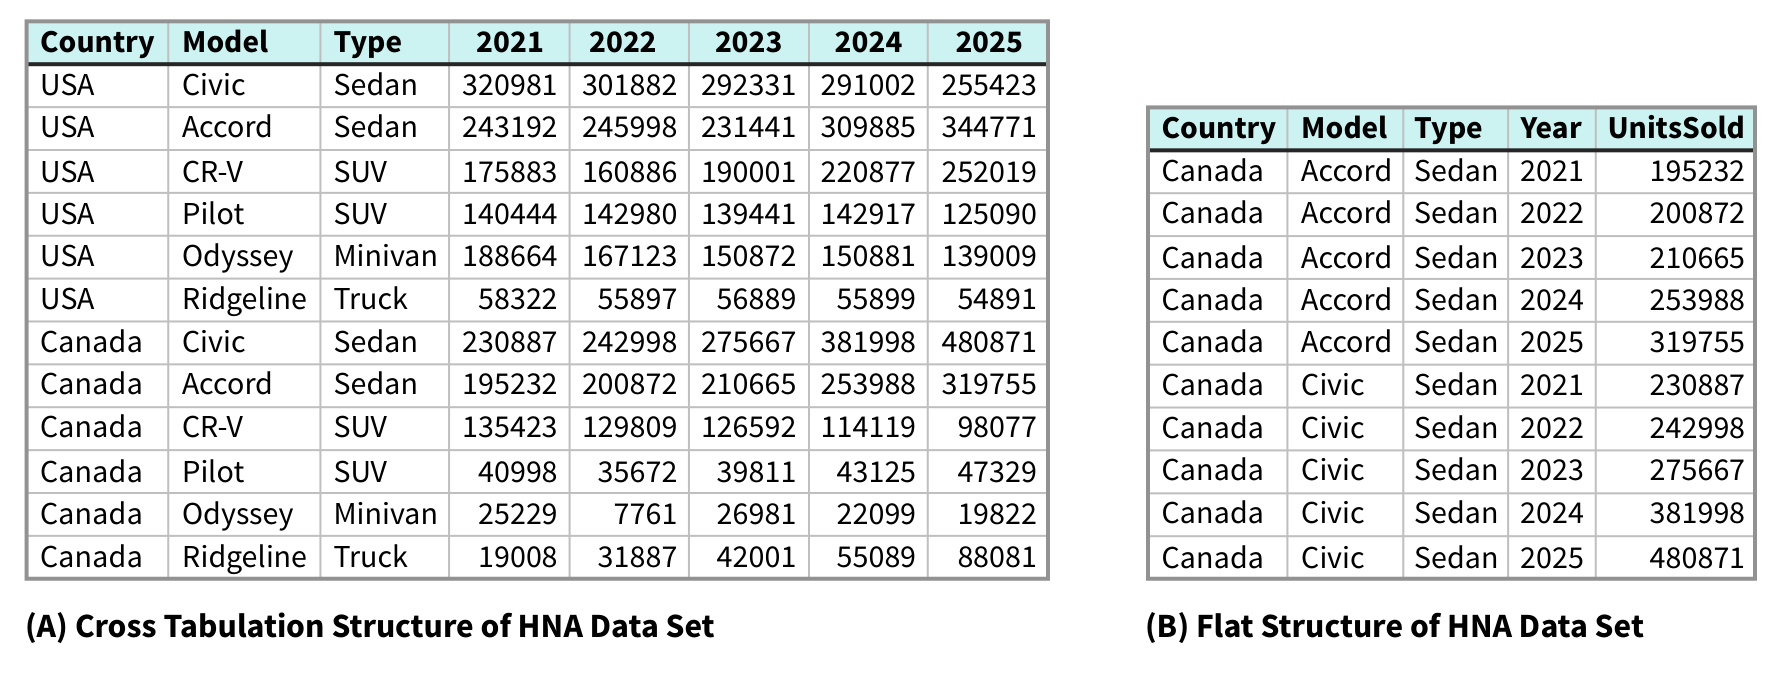
\includegraphics[width=0.95\textwidth,height=0.75\textheight,keepaspectratio]{../textbookForPractice/Figures/Ch_07/ILLUSTRATION 7.2.png}
    \end{figure}
\end{frame}

\begin{frame}{ILLUSTRATION 7.3}

    \begin{figure}[h]
        \centering
        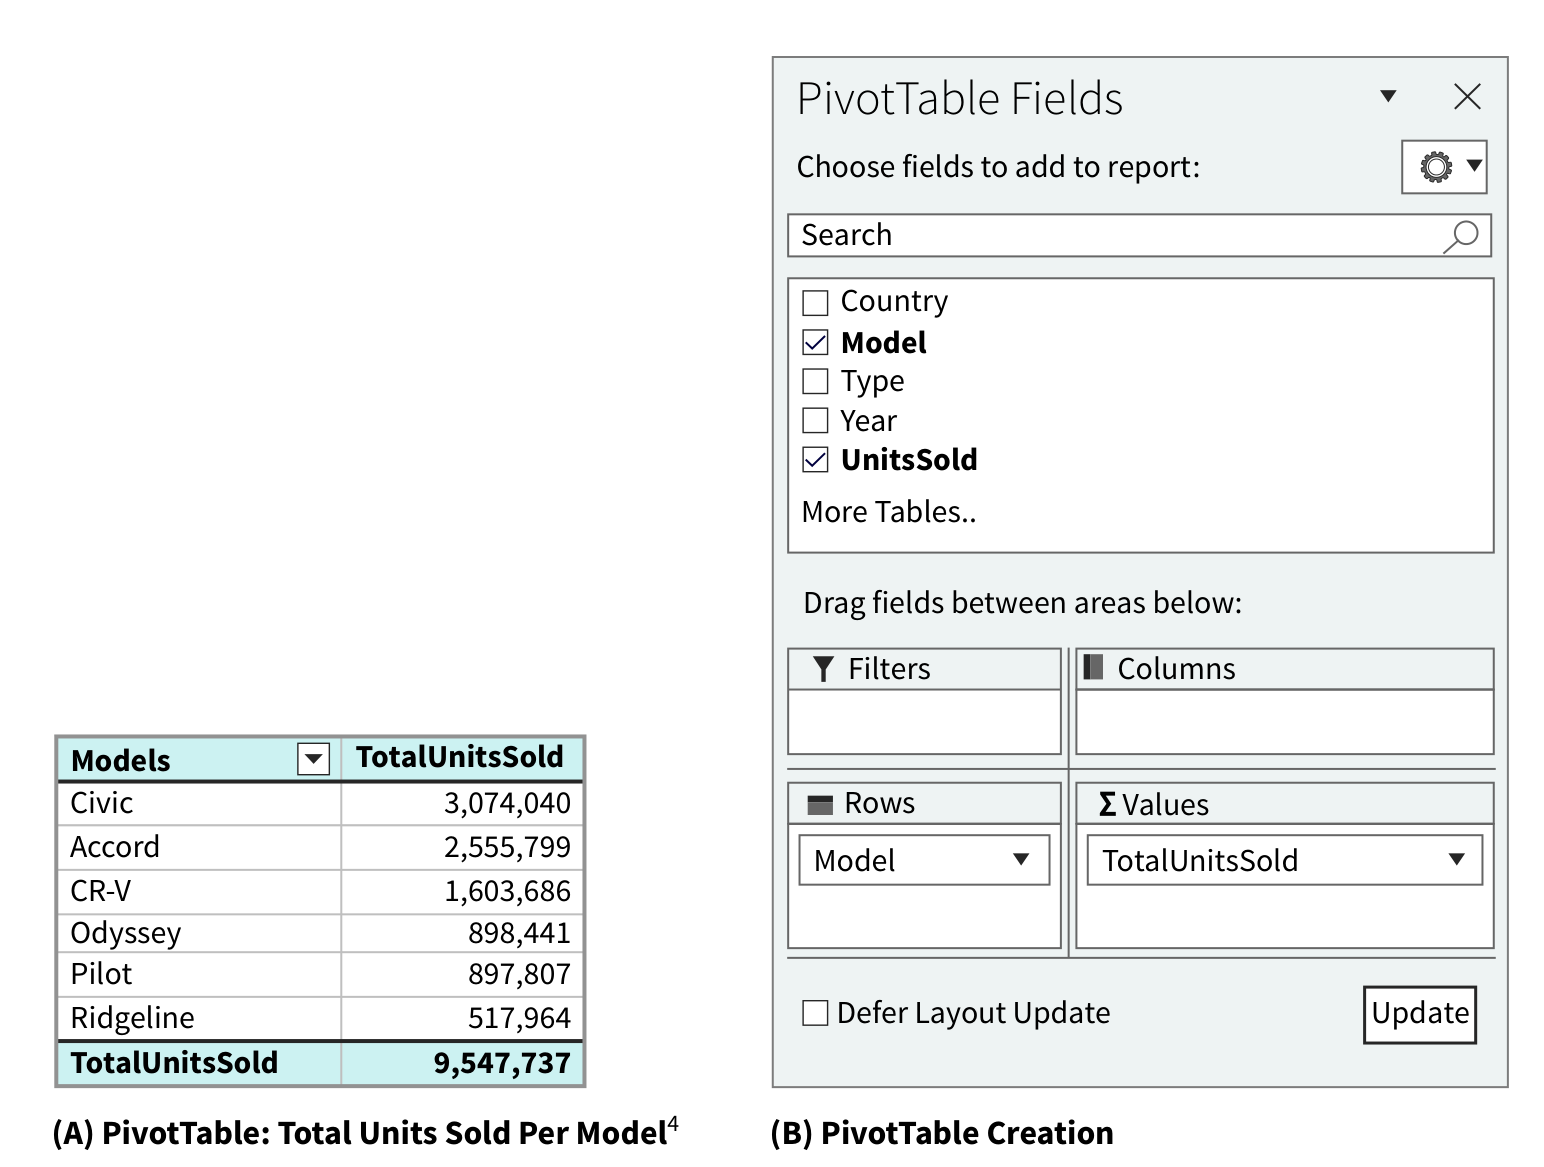
\includegraphics[width=0.95\textwidth,height=0.75\textheight,keepaspectratio]{../textbookForPractice/Figures/Ch_07/ILLUSTRATION 7.3.png}
    \end{figure}
\end{frame}

\begin{frame}{ILLUSTRATION 7.4}

    \begin{figure}[h]
        \centering
        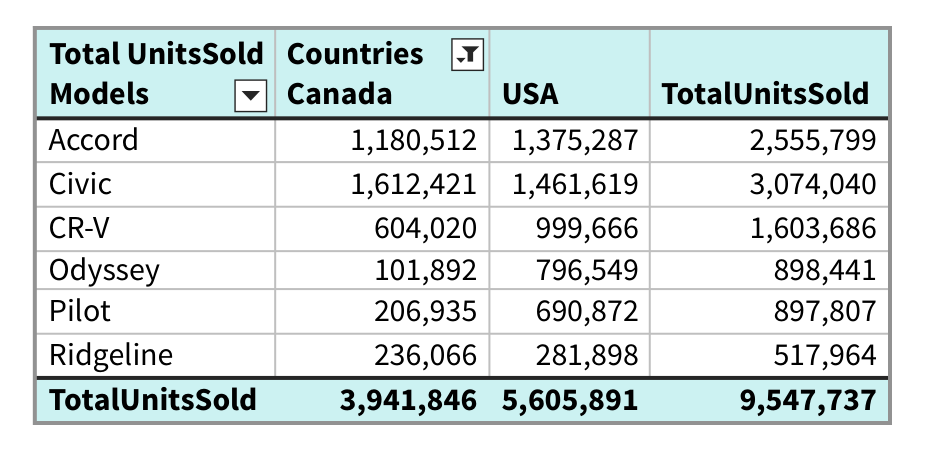
\includegraphics[width=0.95\textwidth,height=0.75\textheight,keepaspectratio]{../textbookForPractice/Figures/Ch_07/ILLUSTRATION 7.4.png}
    \end{figure}
\end{frame}

\begin{frame}{ILLUSTRATION 7.5}

    \begin{figure}[h]
        \centering
        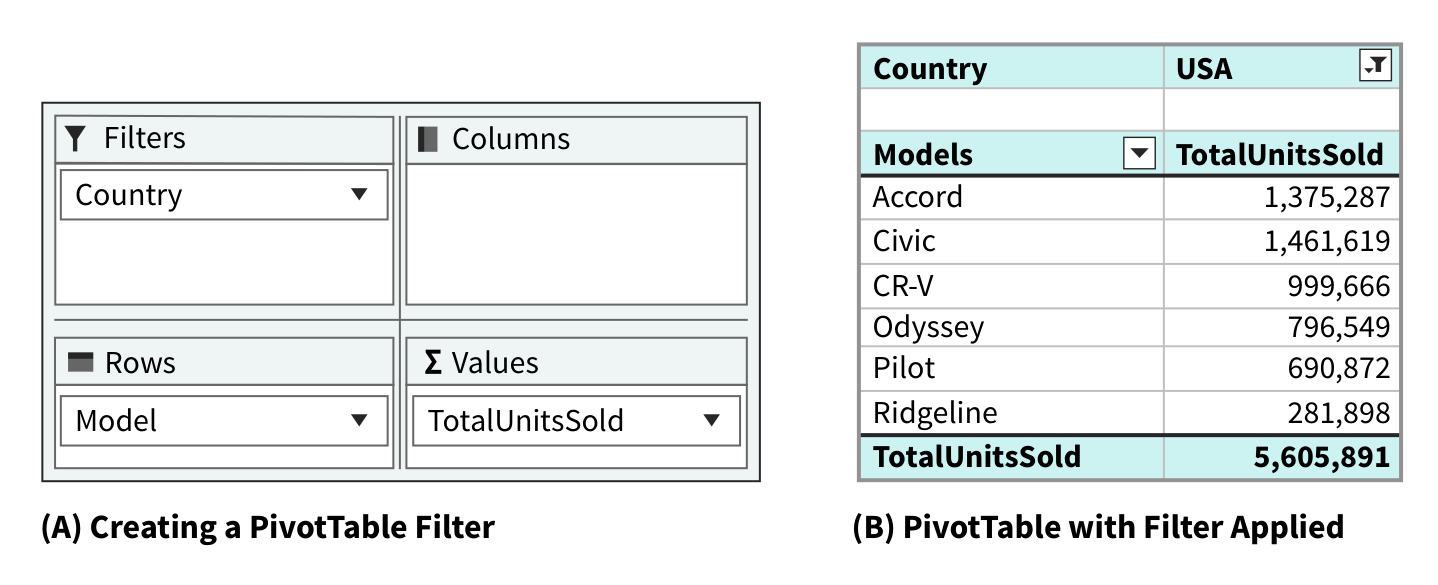
\includegraphics[width=0.95\textwidth,height=0.75\textheight,keepaspectratio]{../textbookForPractice/Figures/Ch_07/ILLUSTRATION 7.5.png}
    \end{figure}
\end{frame}

\begin{frame}{ILLUSTRATION 7.6}

    \begin{figure}[h]
        \centering
        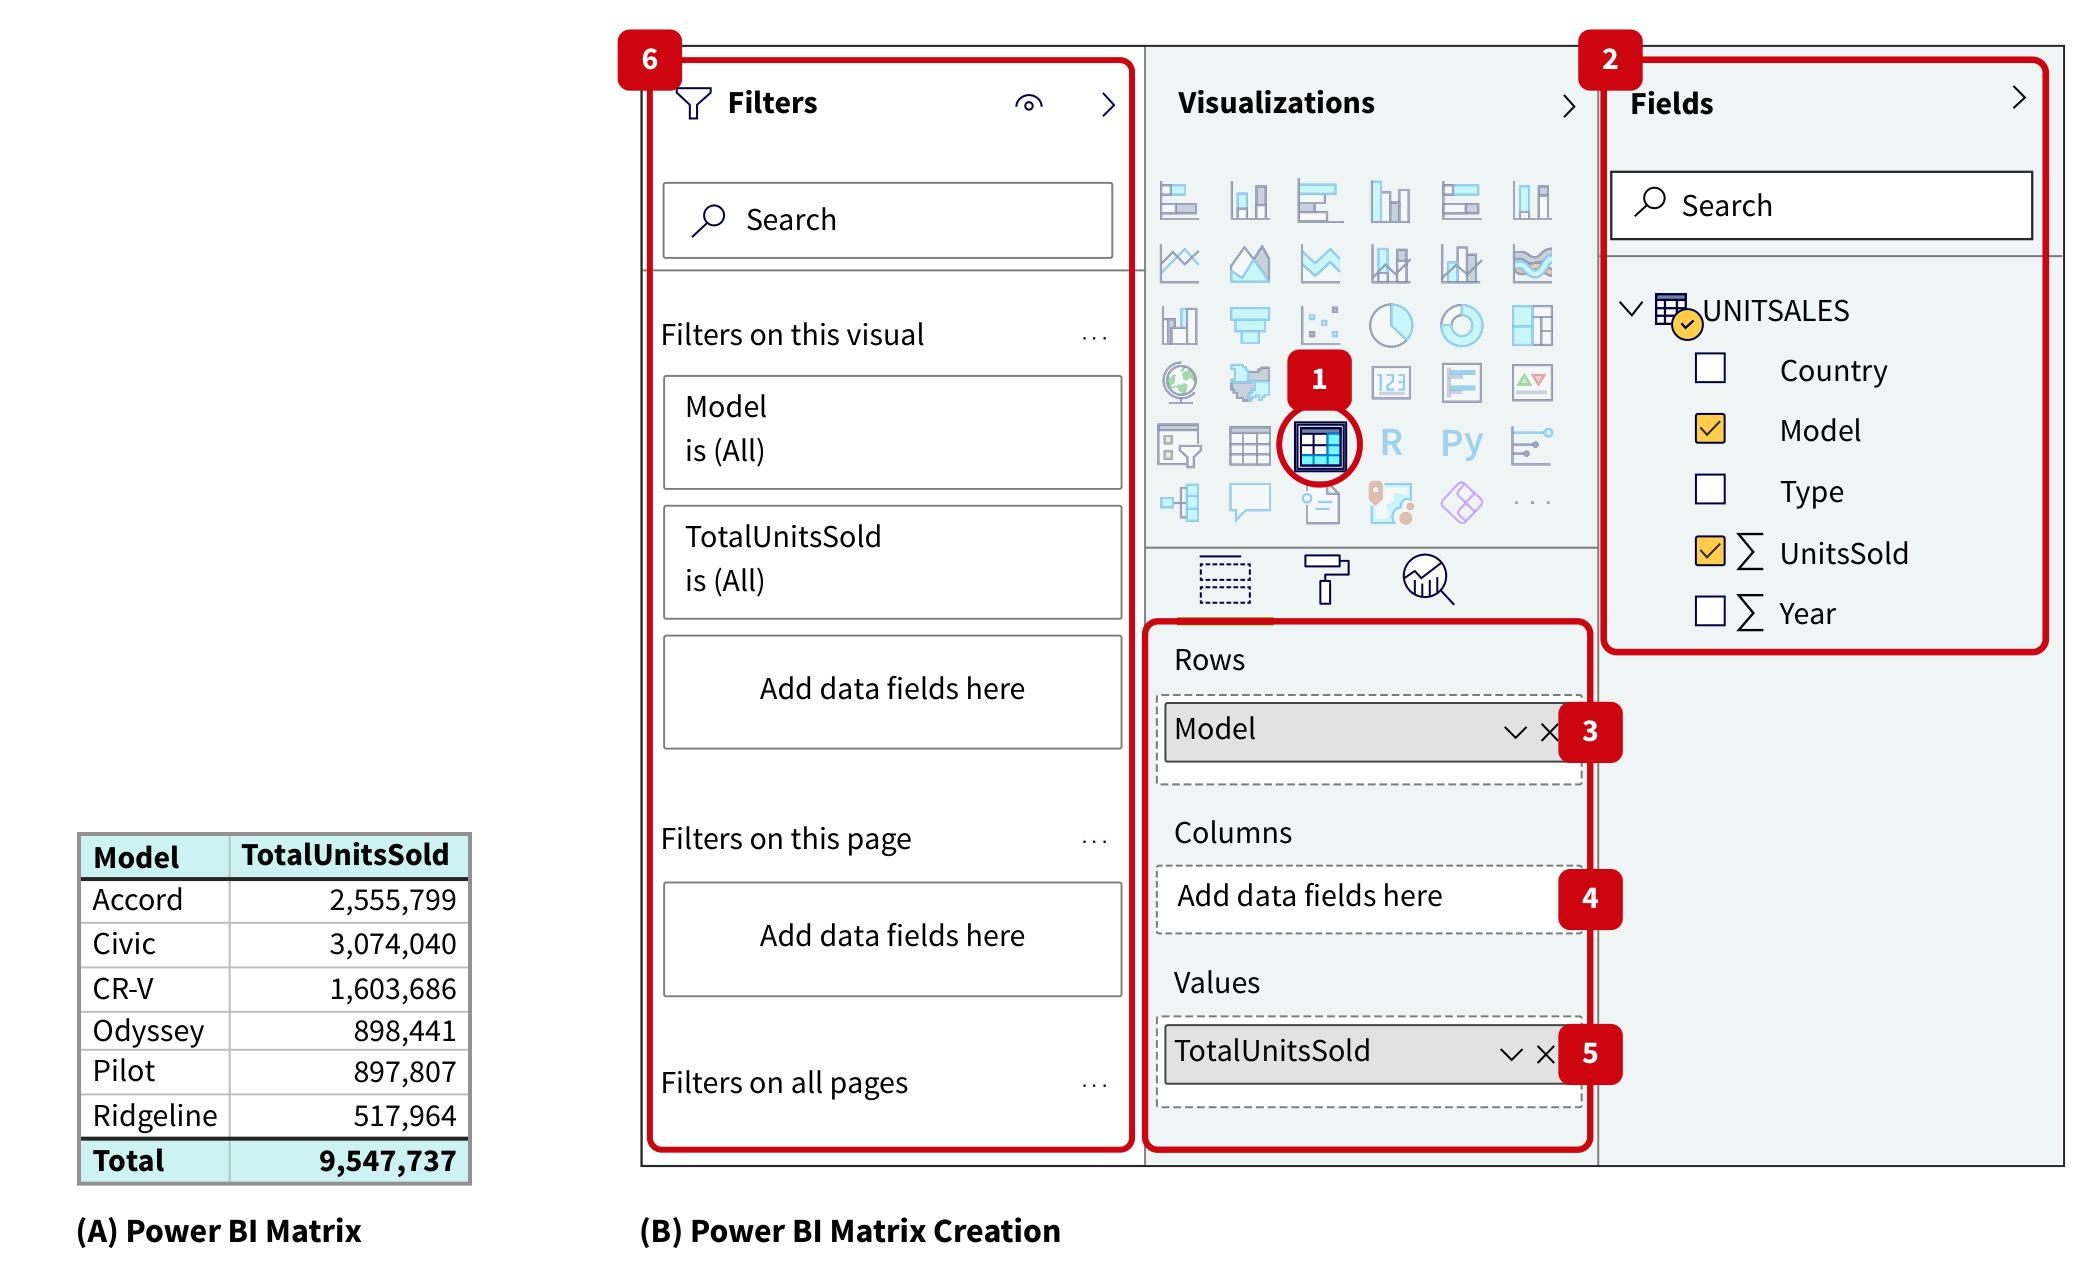
\includegraphics[width=0.95\textwidth,height=0.75\textheight,keepaspectratio]{../textbookForPractice/Figures/Ch_07/ILLUSTRATION 7.6.png}
    \end{figure}
\end{frame}

\begin{frame}{Quy trình Khám phá Dữ liệu}
\begin{itemize}
    \item \textbf{Bước 1: Xác định Mục tiêu (Identify Objectives):} Bạn đang tìm kiếm điều gì?
    \item \textbf{Bước 2: Lựa chọn Biến (Select Variables):} Dữ liệu nào cần thiết?
    \item \textbf{Bước 3: Khám phá Trực quan (Visual Exploration):} Sử dụng biểu đồ.
    \item \textbf{Bước 4: Đánh giá \& Tinh chỉnh (Evaluate \& Refine):} Biểu đồ có ý nghĩa không? Có cần thay đổi không?
\end{itemize}
\end{frame}

\begin{frame}{ILLUSTRATION 7.7}

    \begin{figure}[h]
        \centering
        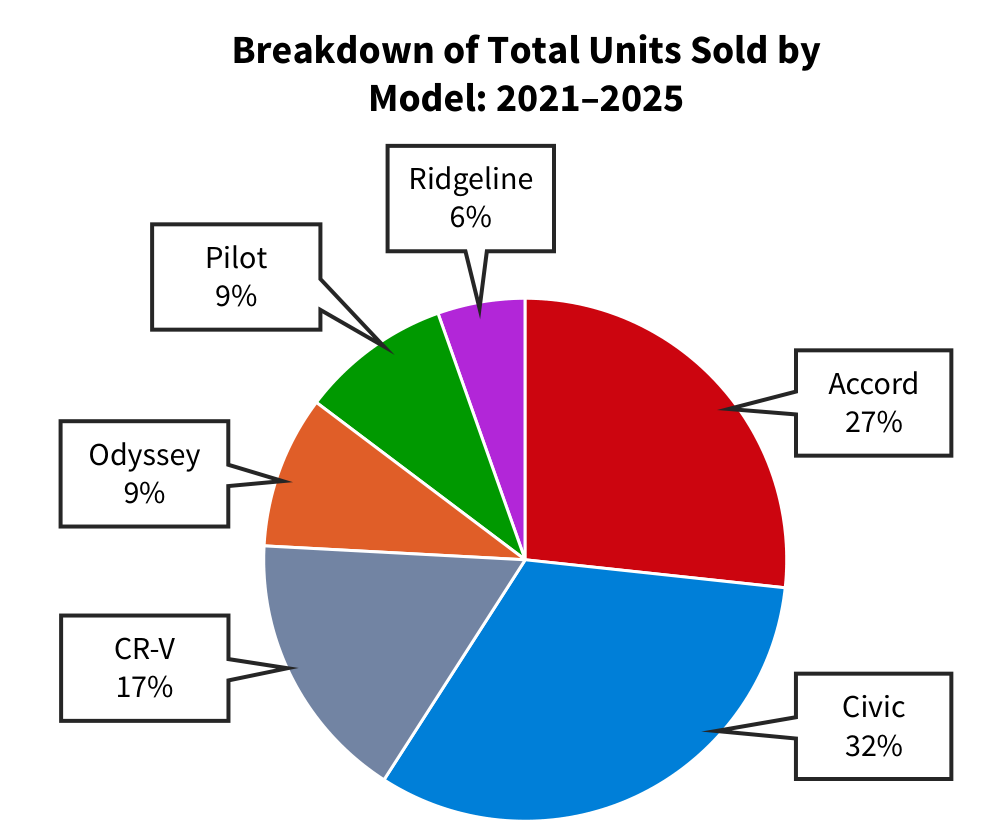
\includegraphics[width=0.95\textwidth,height=0.75\textheight,keepaspectratio]{../textbookForPractice/Figures/Ch_07/ILLUSTRATION 7.7.png}
    \end{figure}
\end{frame}

\begin{frame}{ILLUSTRATION 7.8}

    \begin{figure}[h]
        \centering
        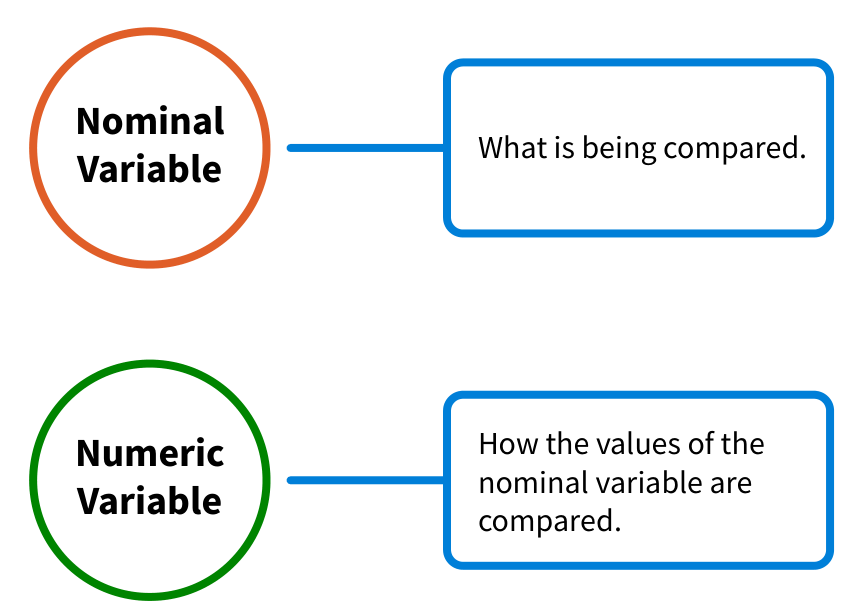
\includegraphics[width=0.95\textwidth,height=0.75\textheight,keepaspectratio]{../textbookForPractice/Figures/Ch_07/ILLUSTRATION 7.8.png}
    \end{figure}
\end{frame}

\begin{frame}{ILLUSTRATION 7.9}

    \begin{figure}[h]
        \centering
        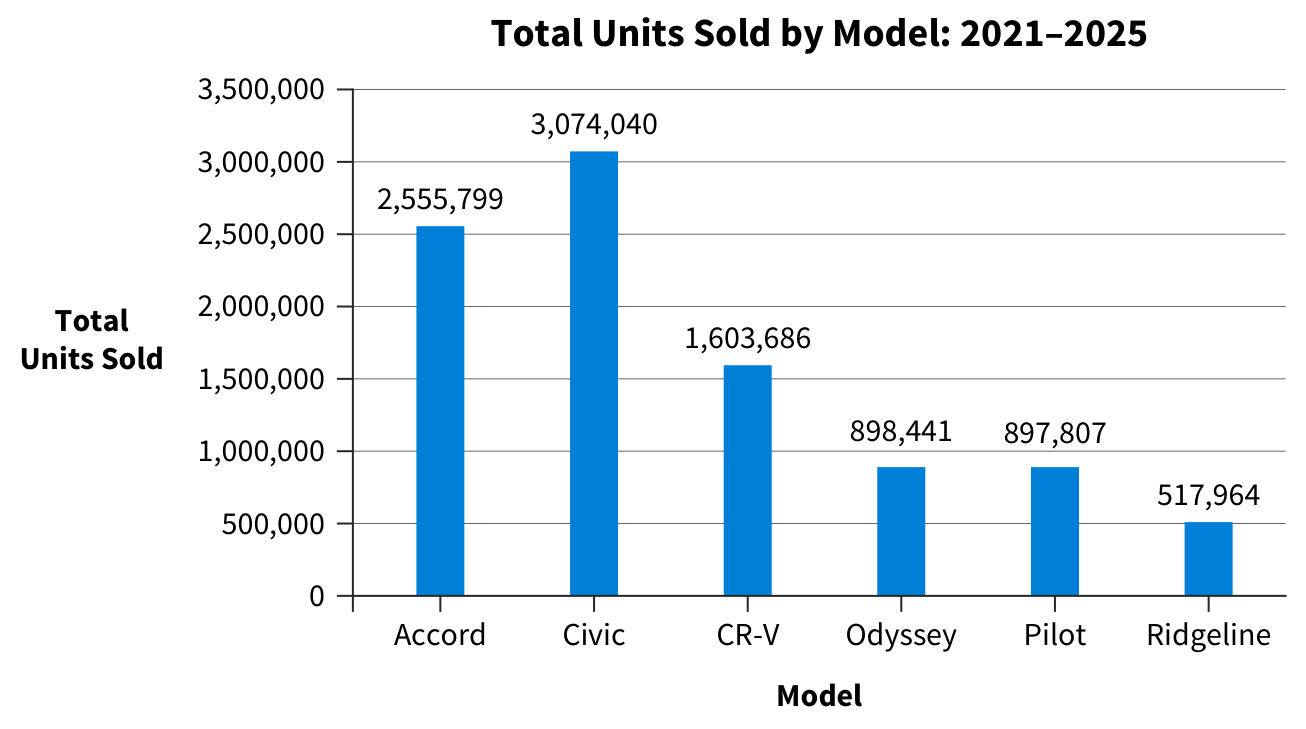
\includegraphics[width=0.95\textwidth,height=0.75\textheight,keepaspectratio]{../textbookForPractice/Figures/Ch_07/ILLUSTRATION 7.9.png}
    \end{figure}
\end{frame}

\begin{frame}{ILLUSTRATION 7.10}

    \begin{figure}[h]
        \centering
        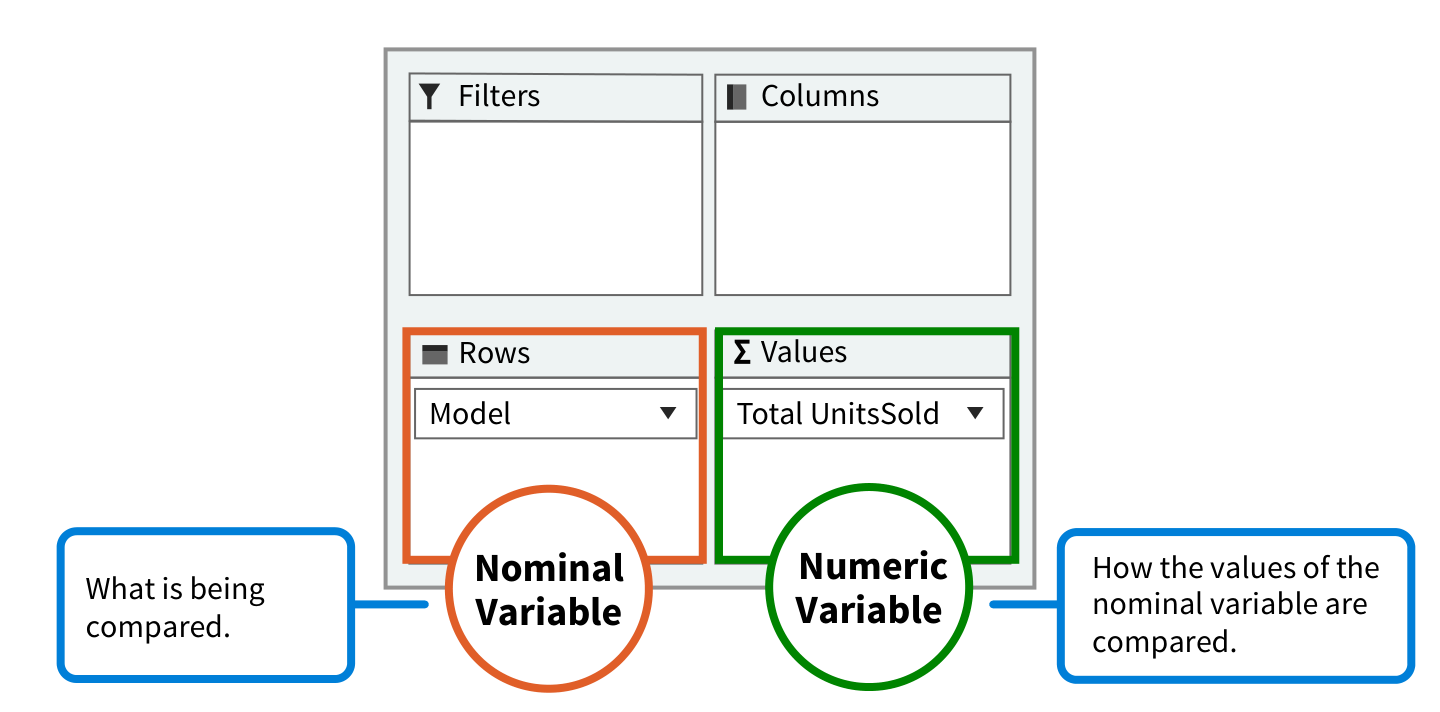
\includegraphics[width=0.95\textwidth,height=0.75\textheight,keepaspectratio]{../textbookForPractice/Figures/Ch_07/ILLUSTRATION 7.10.png}
    \end{figure}
\end{frame}

\begin{frame}{ILLUSTRATION 7.11}

    \begin{figure}[h]
        \centering
        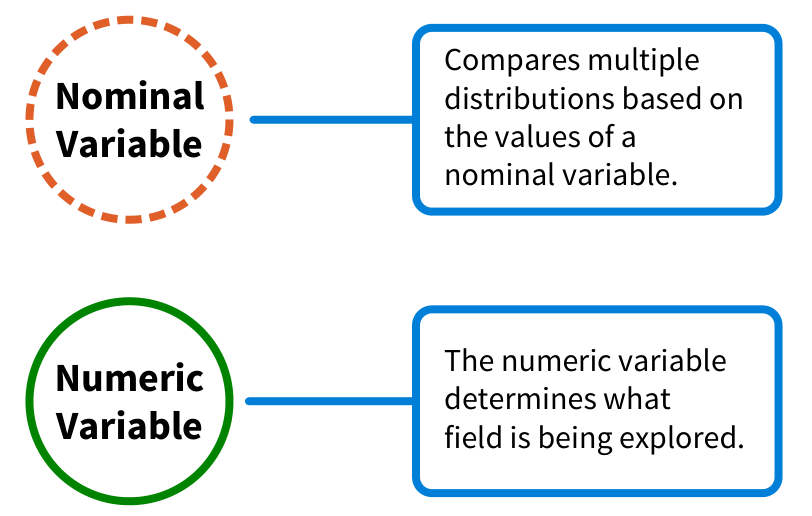
\includegraphics[width=0.95\textwidth,height=0.75\textheight,keepaspectratio]{../textbookForPractice/Figures/Ch_07/ILLUSTRATION 7.11.png}
    \end{figure}
\end{frame}

\begin{frame}{ILLUSTRATION 7.12}

    \begin{figure}[h]
        \centering
        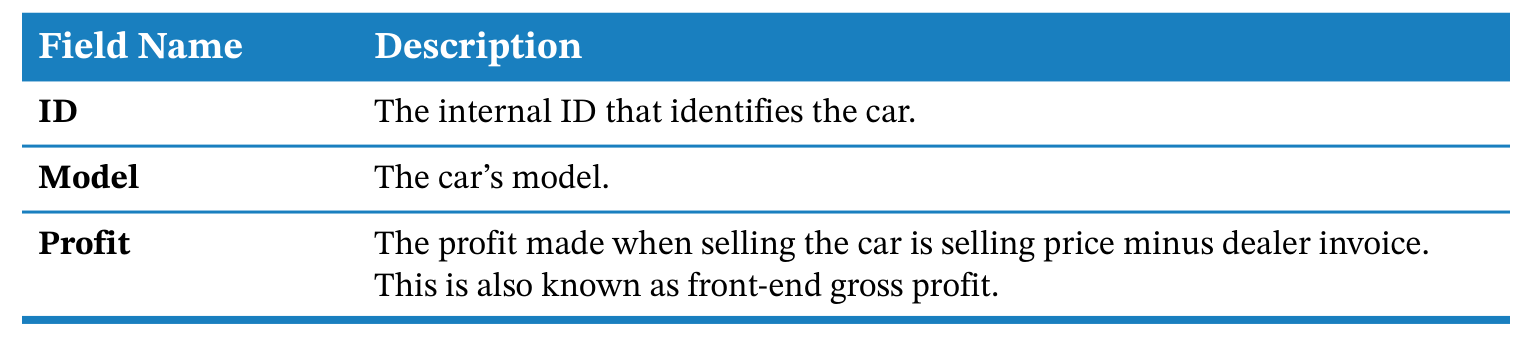
\includegraphics[width=0.95\textwidth,height=0.75\textheight,keepaspectratio]{../textbookForPractice/Figures/Ch_07/ILLUSTRATION 7.12.png}
    \end{figure}
\end{frame}

\begin{frame}{Công cụ Khám phá Dữ liệu}
\begin{itemize}
    \item \textbf{PivotTables trong Excel:} Công cụ cơ bản, nhanh chóng và phổ biến nhất để nhóm, tóm tắt và lọc dữ liệu.
    \item \textbf{Đa nền tảng (Across Tools):} Các công cụ BI hiện đại (Power BI, Tableau) cung cấp khả năng trực quan hóa mạnh mẽ hơn, hỗ trợ tương tác và xử lý dữ liệu lớn (Big Data).
    \item \textbf{Mục tiêu cốt lõi:} Tìm ra các \textit{Insights} ẩn giấu đằng sau những con số tài chính khô khan.
\end{itemize}
\end{frame}

\begin{frame}{ILLUSTRATION 7.13}

    \begin{figure}[h]
        \centering
        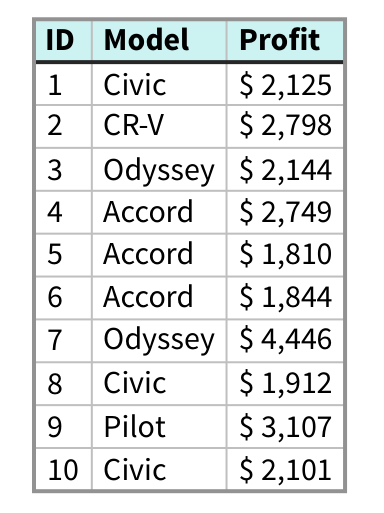
\includegraphics[width=0.95\textwidth,height=0.75\textheight,keepaspectratio]{../textbookForPractice/Figures/Ch_07/ILLUSTRATION 7.13.png}
    \end{figure}
\end{frame}

\begin{frame}{ILLUSTRATION 7.14}

    \begin{figure}[h]
        \centering
        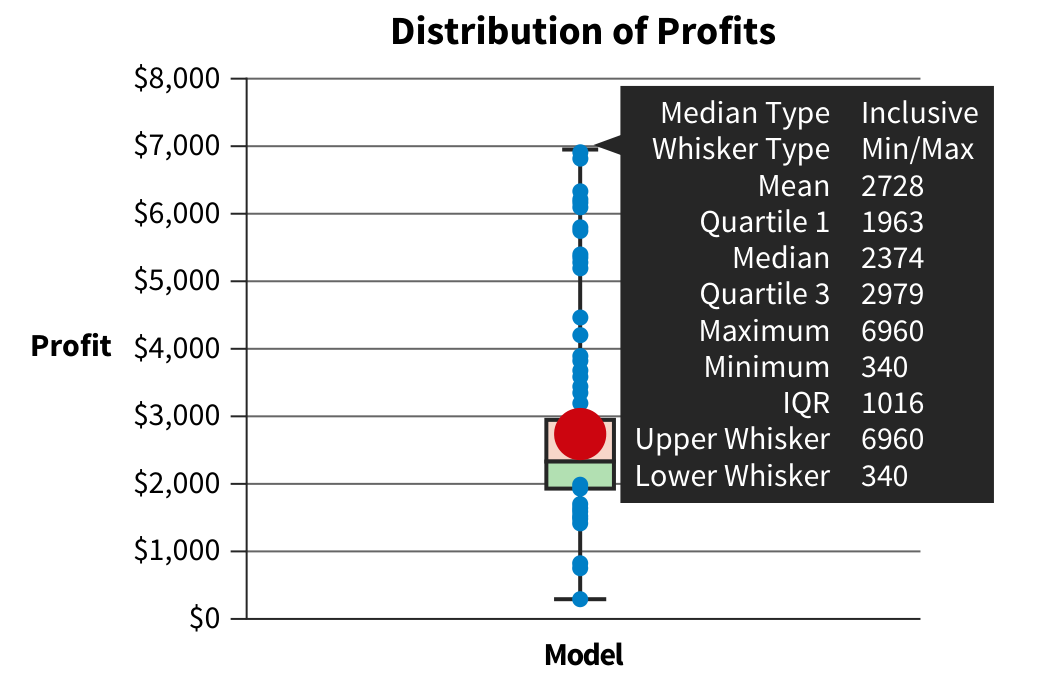
\includegraphics[width=0.95\textwidth,height=0.75\textheight,keepaspectratio]{../textbookForPractice/Figures/Ch_07/ILLUSTRATION 7.14.png}
    \end{figure}
\end{frame}

\begin{frame}{ILLUSTRATION 7.15}

    \begin{figure}[h]
        \centering
        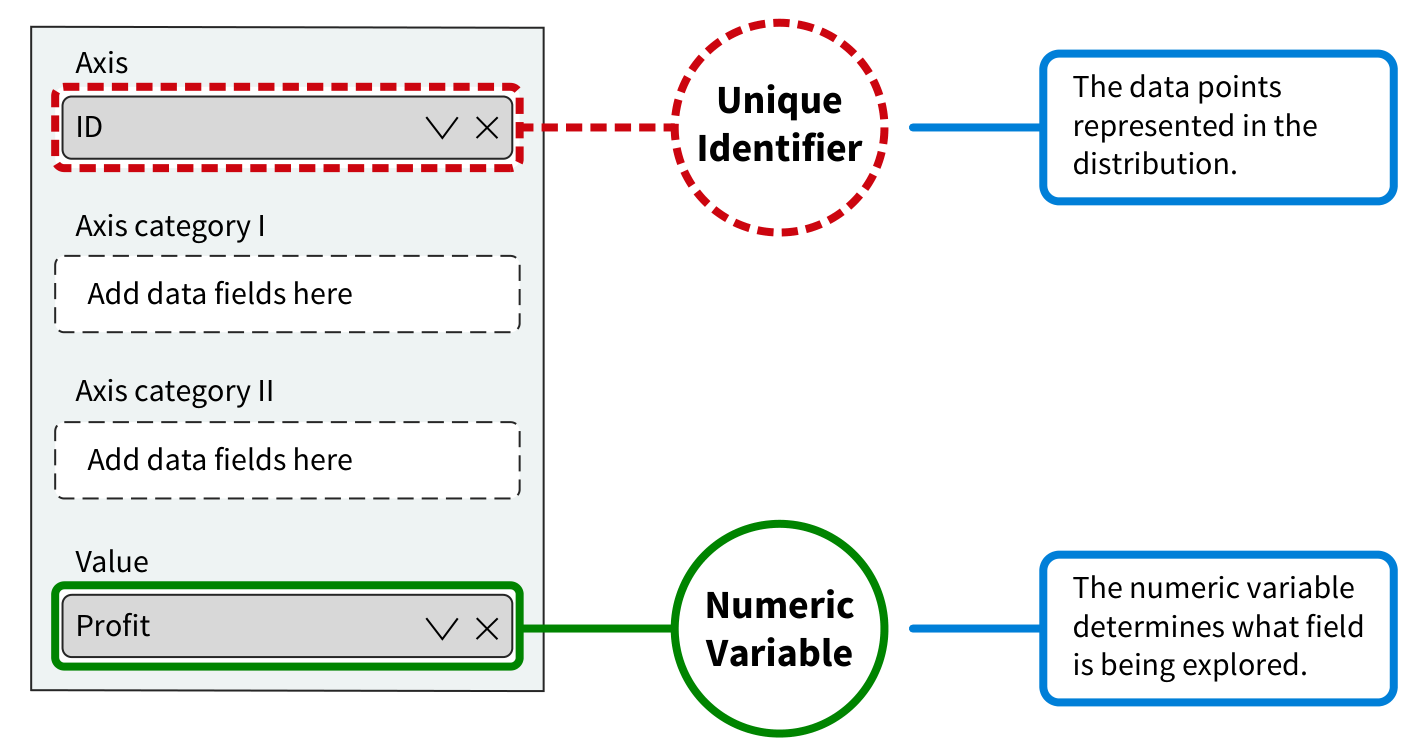
\includegraphics[width=0.95\textwidth,height=0.75\textheight,keepaspectratio]{../textbookForPractice/Figures/Ch_07/ILLUSTRATION 7.15.png}
    \end{figure}
\end{frame}

\begin{frame}{ILLUSTRATION 7.16}

    \begin{figure}[h]
        \centering
        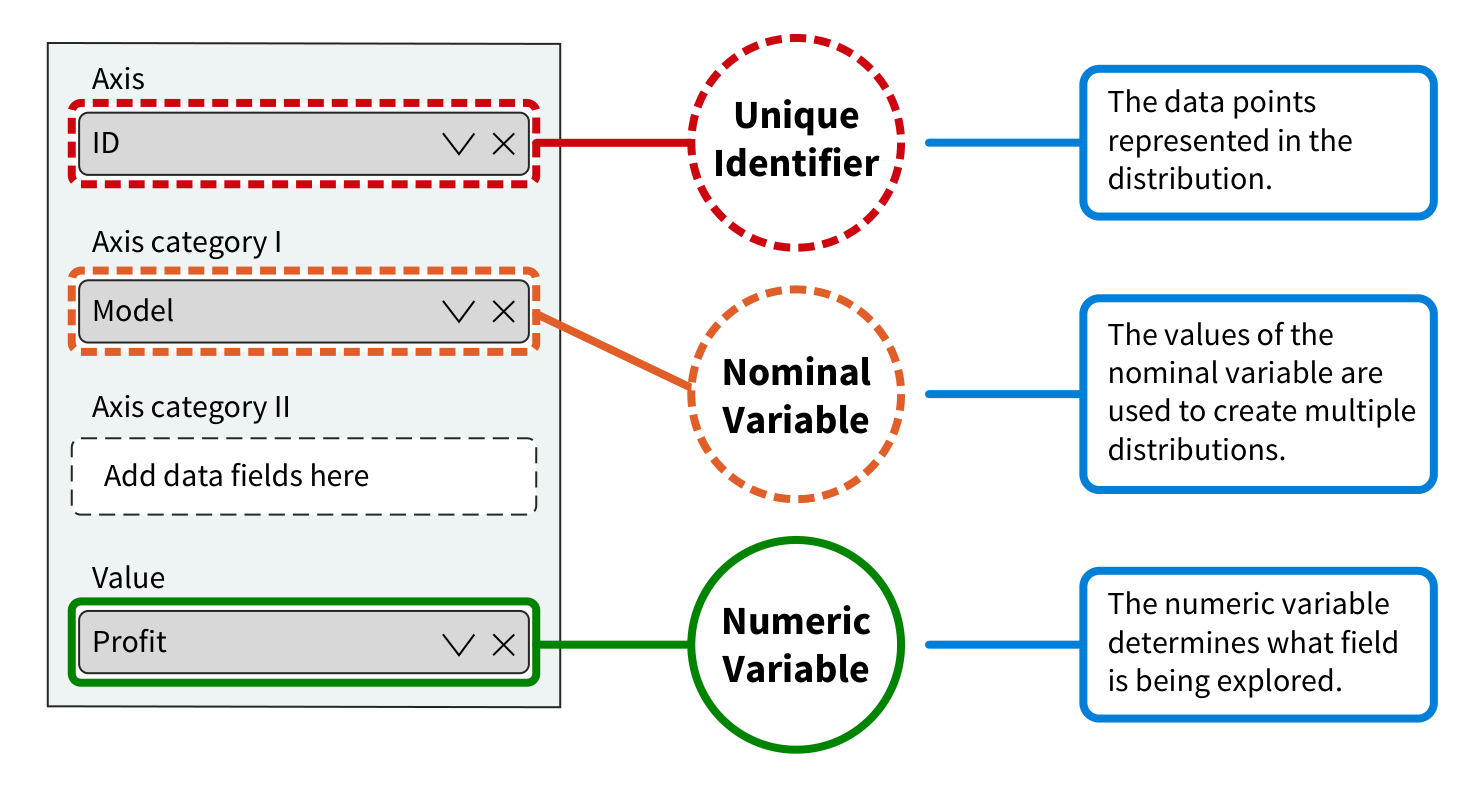
\includegraphics[width=0.95\textwidth,height=0.75\textheight,keepaspectratio]{../textbookForPractice/Figures/Ch_07/ILLUSTRATION 7.16.png}
    \end{figure}
\end{frame}

\begin{frame}{ILLUSTRATION 7.17}

    \begin{figure}[h]
        \centering
        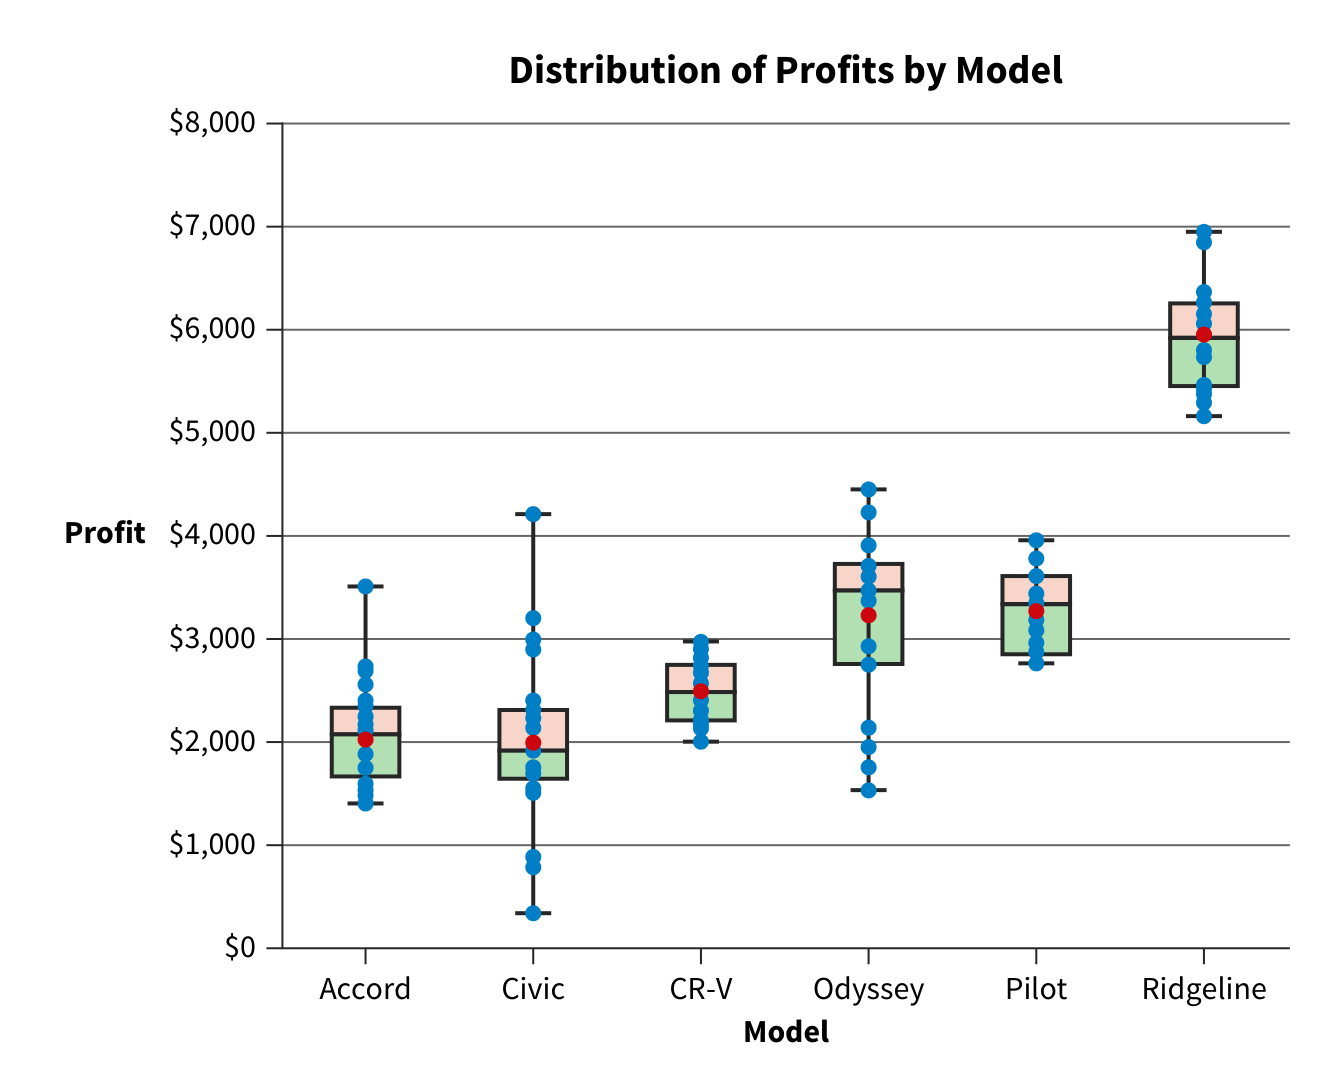
\includegraphics[width=0.95\textwidth,height=0.75\textheight,keepaspectratio]{../textbookForPractice/Figures/Ch_07/ILLUSTRATION 7.17.png}
    \end{figure}
\end{frame}

\begin{frame}{7.2 Mối quan hệ Nền tảng qua Trực quan hóa}
\begin{itemize}
    \item \textbf{Mục đích:} Giúp não bộ con người nhanh chóng nhận diện quy luật (Pattern Recognition).
    \item \textbf{8 Mẫu Mối quan hệ Nền tảng (Eight Patterns):}
    \begin{enumerate}
        \item Phần-Toàn thể (Part-To-Whole)
        \item So sánh Cường độ (Magnitude)
        \item Chuỗi Thời gian (Time Series)
        \item Phân phối (Distribution)
        \item ... và 4 mẫu nâng cao khác.
    \end{enumerate}
\end{itemize}
\end{frame}

\begin{frame}{ILLUSTRATION 7.18}

    \begin{figure}[h]
        \centering
        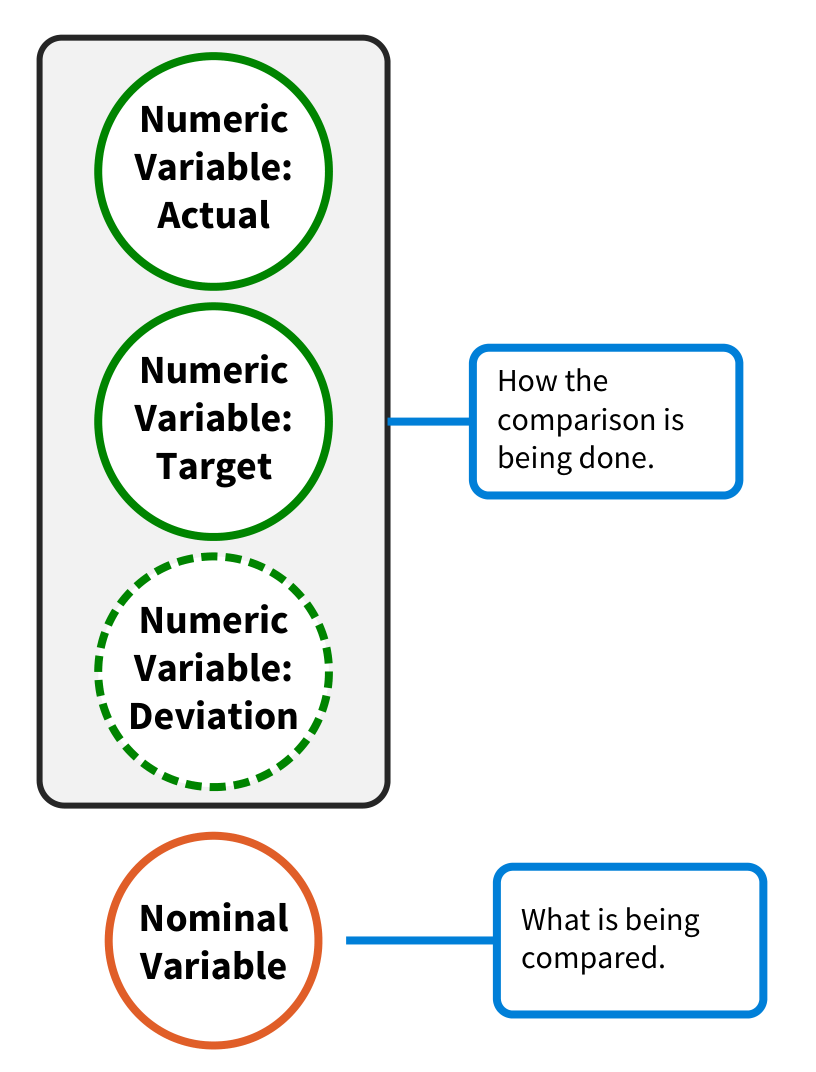
\includegraphics[width=0.95\textwidth,height=0.75\textheight,keepaspectratio]{../textbookForPractice/Figures/Ch_07/ILLUSTRATION 7.18.png}
    \end{figure}
\end{frame}

\begin{frame}{ILLUSTRATION 7.19}

    \begin{figure}[h]
        \centering
        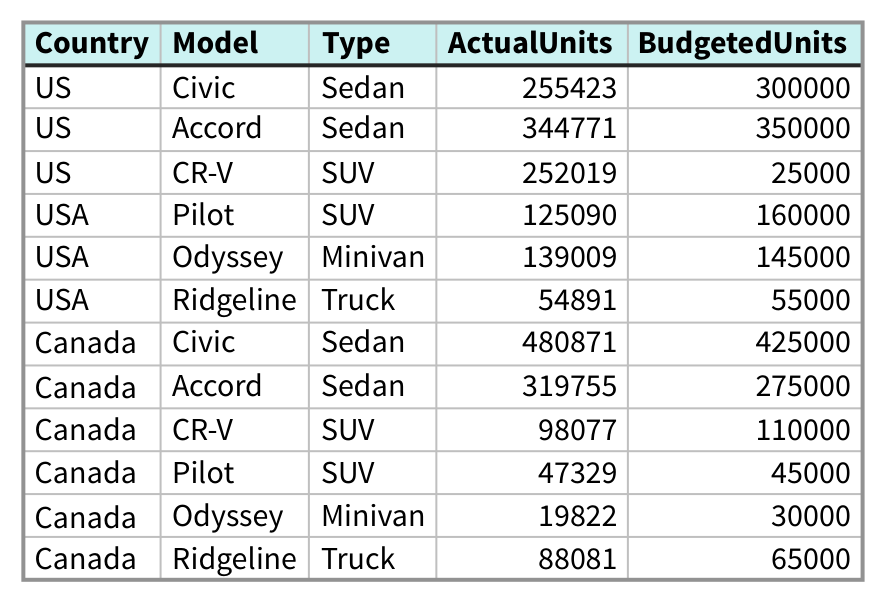
\includegraphics[width=0.95\textwidth,height=0.75\textheight,keepaspectratio]{../textbookForPractice/Figures/Ch_07/ILLUSTRATION 7.19.png}
    \end{figure}
\end{frame}

\begin{frame}{ILLUSTRATION 7.20}

    \begin{figure}[h]
        \centering
        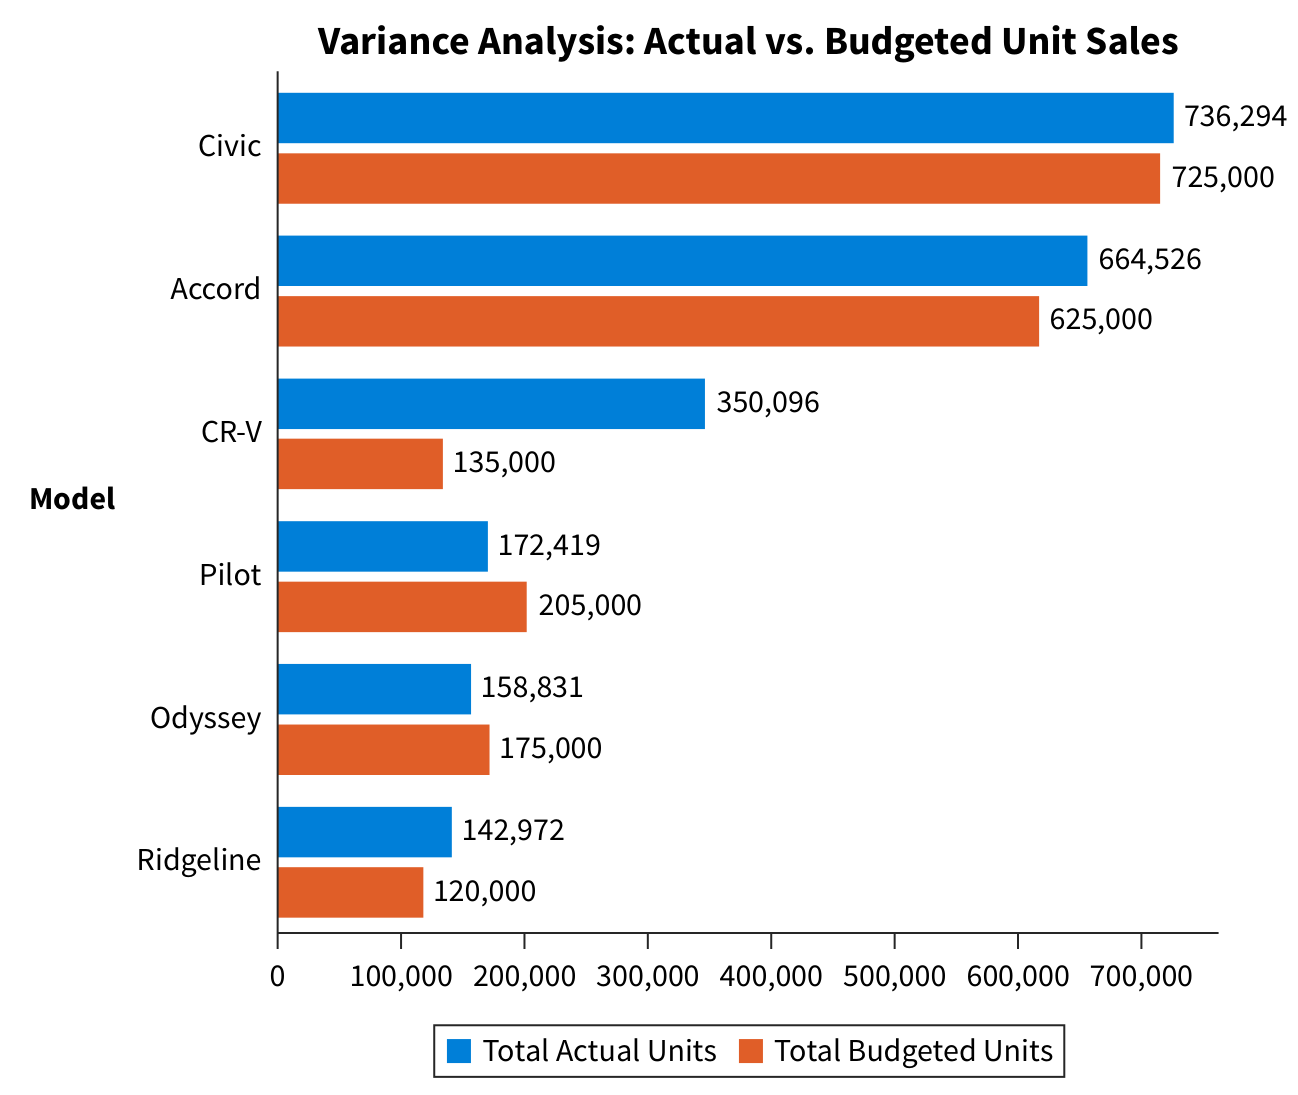
\includegraphics[width=0.95\textwidth,height=0.75\textheight,keepaspectratio]{../textbookForPractice/Figures/Ch_07/ILLUSTRATION 7.20.png}
    \end{figure}
\end{frame}

\begin{frame}{ILLUSTRATION 7.21}

    \begin{figure}[h]
        \centering
        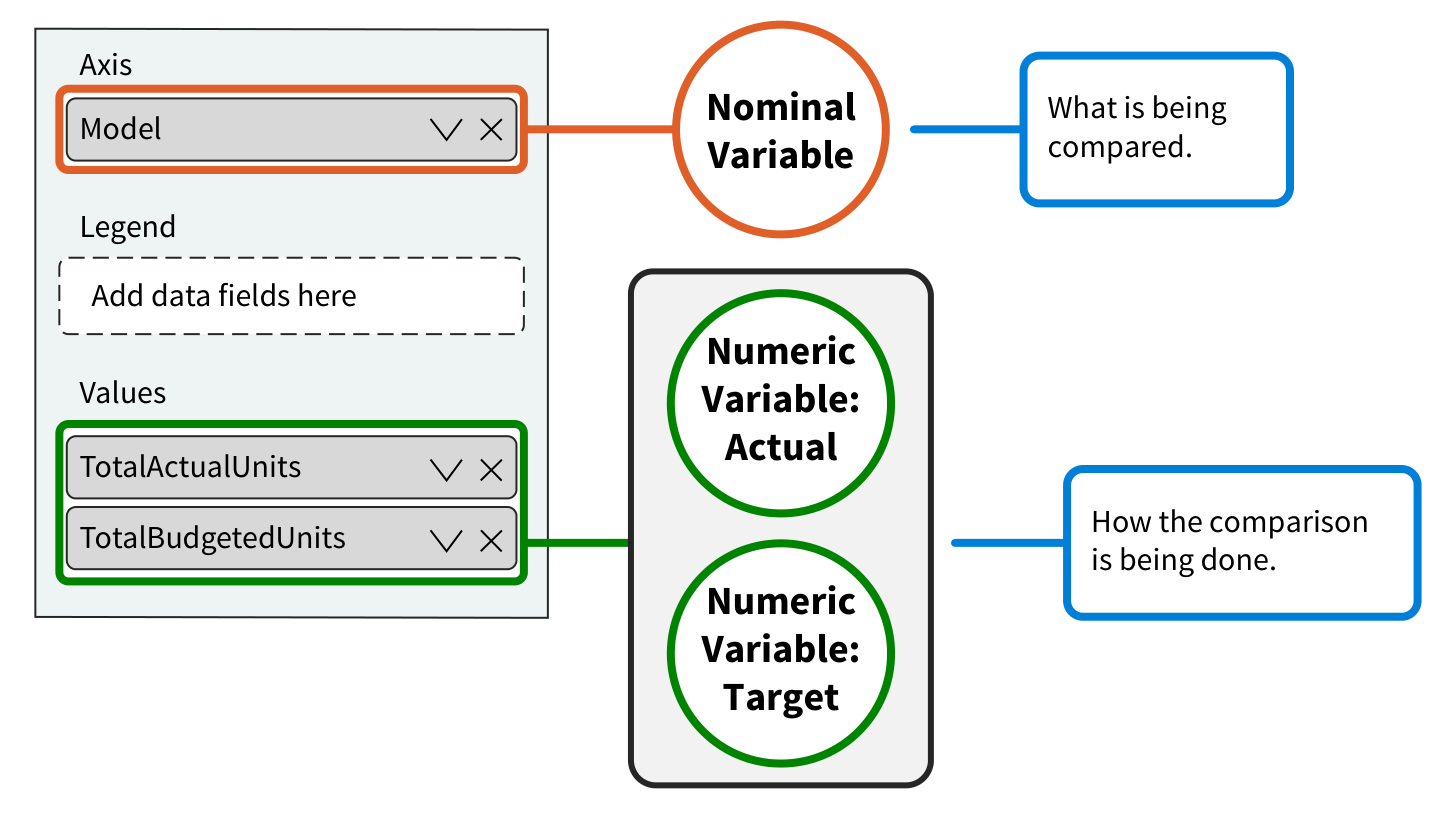
\includegraphics[width=0.95\textwidth,height=0.75\textheight,keepaspectratio]{../textbookForPractice/Figures/Ch_07/ILLUSTRATION 7.21.png}
    \end{figure}
\end{frame}

\begin{frame}{ILLUSTRATION 7.22}

    \begin{figure}[h]
        \centering
        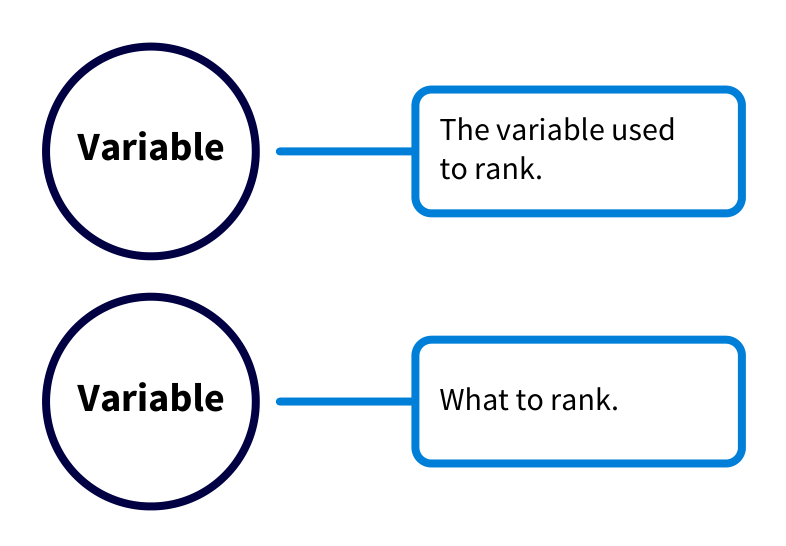
\includegraphics[width=0.95\textwidth,height=0.75\textheight,keepaspectratio]{../textbookForPractice/Figures/Ch_07/ILLUSTRATION 7.22.png}
    \end{figure}
\end{frame}

\begin{frame}{Phân tích Các Mẫu Cơ bản}
\begin{itemize}
    \item \textbf{Phần-Toàn thể (Part-To-Whole):} Biểu đồ tròn (Pie), Biểu đồ vành khăn (Donut), Treemap. Cho thấy tỷ trọng đóng góp (Ví dụ: Tỷ trọng doanh thu theo từng sản phẩm).
    \item \textbf{Cường độ (Magnitude):} Biểu đồ cột (Bar/Column). Dùng để so sánh trực diện kích thước, quy mô giữa các hạng mục.
    \item \textbf{Chuỗi Thời gian (Time Series):} Biểu đồ đường (Line). Thể hiện xu hướng biến động qua thời gian (Tháng, Quý, Năm).
\end{itemize}
\end{frame}

\begin{frame}{ILLUSTRATION 7.23}

    \begin{figure}[h]
        \centering
        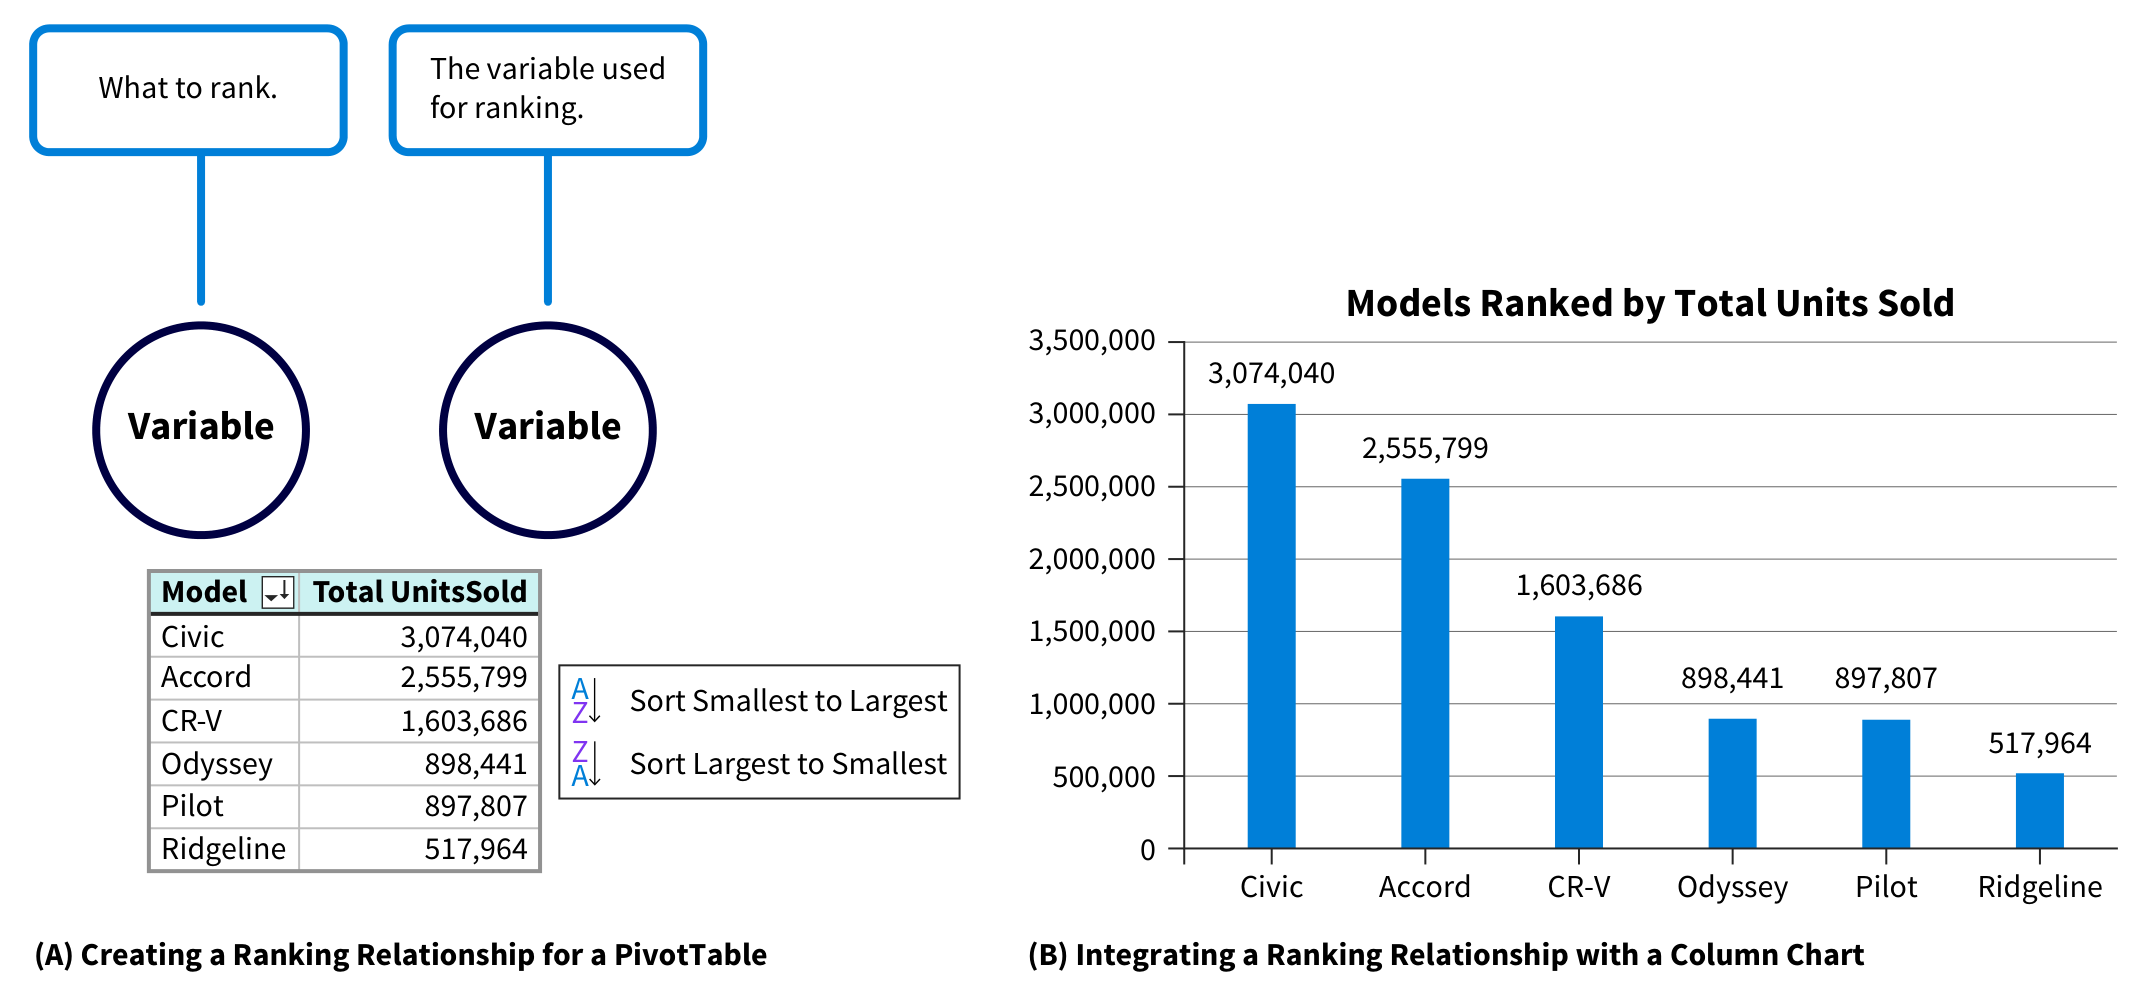
\includegraphics[width=0.95\textwidth,height=0.75\textheight,keepaspectratio]{../textbookForPractice/Figures/Ch_07/ILLUSTRATION 7.23.png}
    \end{figure}
\end{frame}

\begin{frame}{ILLUSTRATION 7.24}

    \begin{figure}[h]
        \centering
        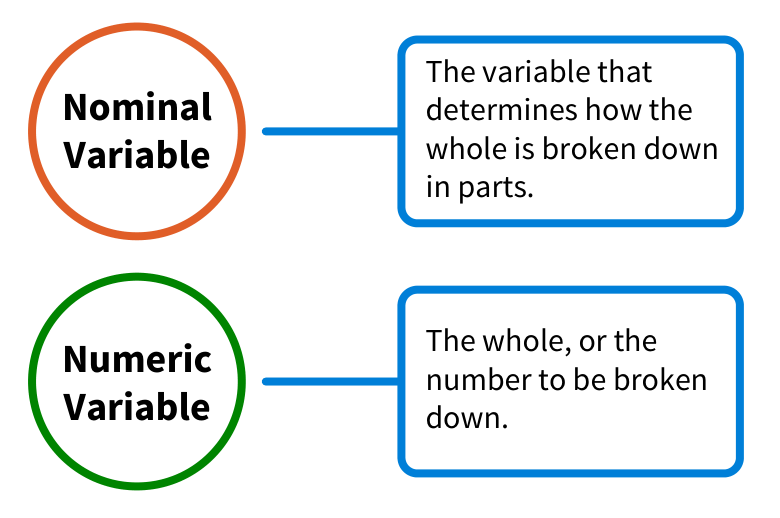
\includegraphics[width=0.95\textwidth,height=0.75\textheight,keepaspectratio]{../textbookForPractice/Figures/Ch_07/ILLUSTRATION 7.24.png}
    \end{figure}
\end{frame}

\begin{frame}{ILLUSTRATION 7.25}

    \begin{figure}[h]
        \centering
        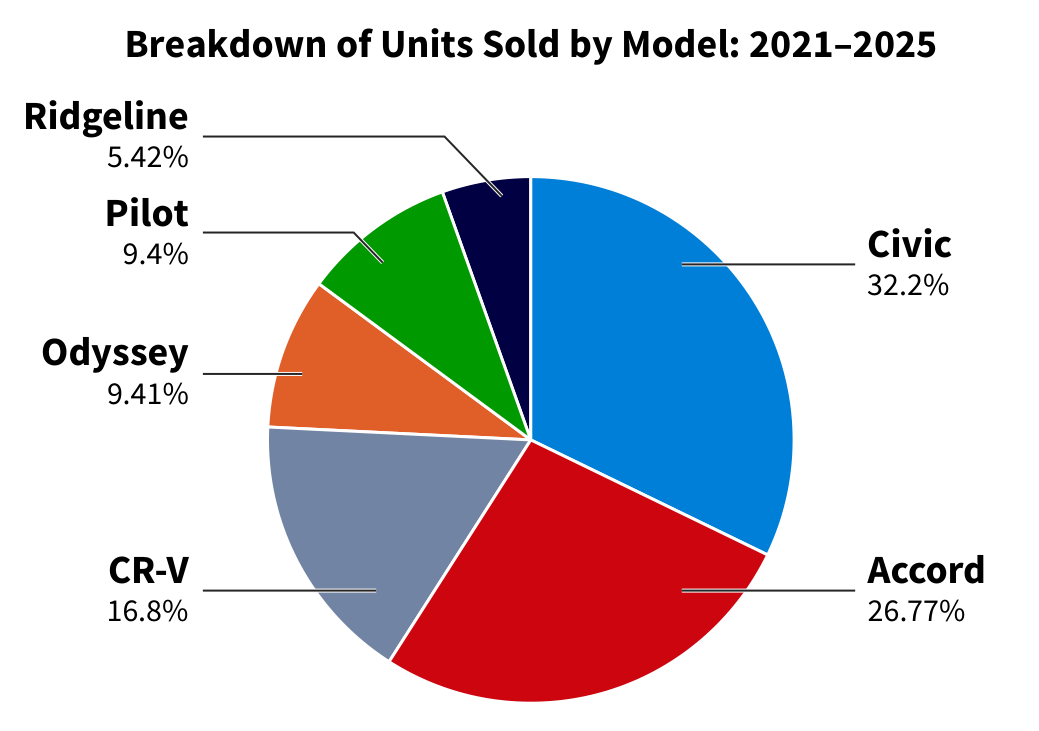
\includegraphics[width=0.95\textwidth,height=0.75\textheight,keepaspectratio]{../textbookForPractice/Figures/Ch_07/ILLUSTRATION 7.25.png}
    \end{figure}
\end{frame}

\begin{frame}{ILLUSTRATION 7.26}

    \begin{figure}[h]
        \centering
        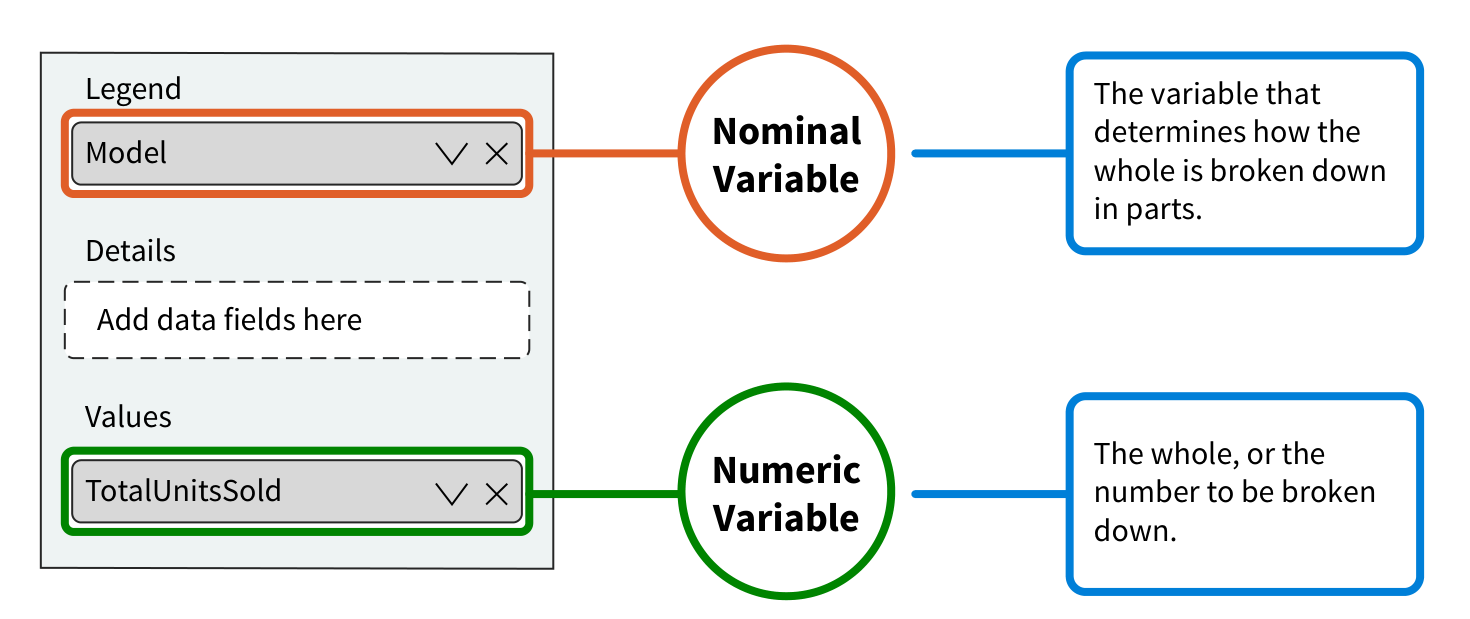
\includegraphics[width=0.95\textwidth,height=0.75\textheight,keepaspectratio]{../textbookForPractice/Figures/Ch_07/ILLUSTRATION 7.26.png}
    \end{figure}
\end{frame}

\begin{frame}{Phân tích Các Mẫu Nâng cao}
\begin{itemize}
    \item \textbf{Phân phối (Distribution):} Biểu đồ Histogram, Box-plot. Đánh giá sự phân tán của dữ liệu và phát hiện ngoại lai (Outliers).
    \item \textbf{Tương quan (Correlation):} Biểu đồ phân tán (Scatter plot). Kiểm tra mối liên hệ giữa hai biến (Ví dụ: Chi phí quảng cáo và Doanh thu).
    \item \textbf{Không gian/Địa lý (Spatial):} Bản đồ (Map). Hiển thị dữ liệu theo vị trí địa lý (Ví dụ: Doanh số theo Tỉnh/Thành phố).
\end{itemize}
\end{frame}

\begin{frame}{ILLUSTRATION 7.27}

    \begin{figure}[h]
        \centering
        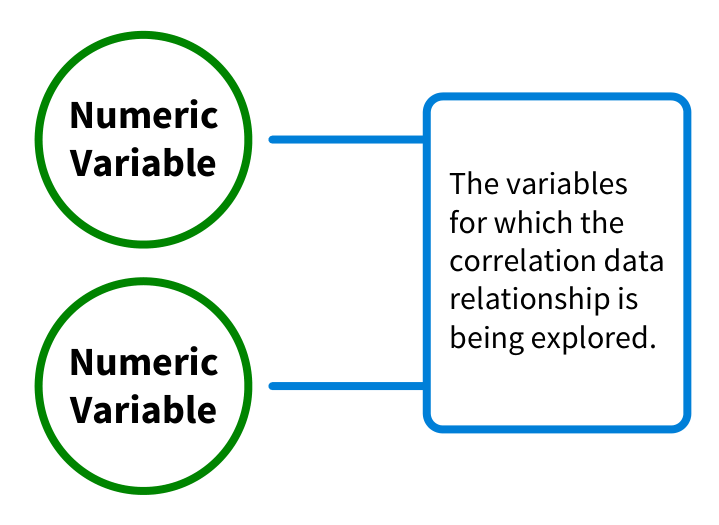
\includegraphics[width=0.95\textwidth,height=0.75\textheight,keepaspectratio]{../textbookForPractice/Figures/Ch_07/ILLUSTRATION 7.27.png}
    \end{figure}
\end{frame}

\begin{frame}{ILLUSTRATION 7.28}

    \begin{figure}[h]
        \centering
        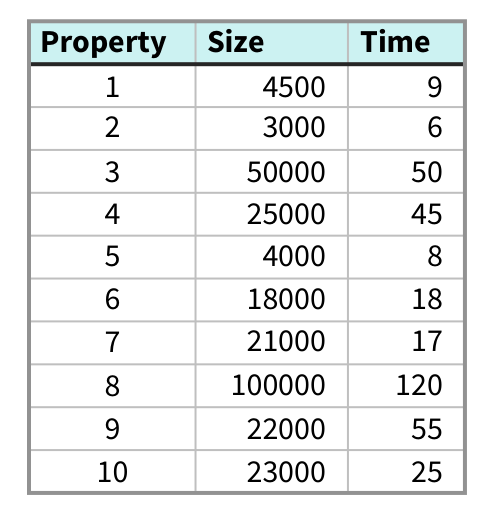
\includegraphics[width=0.95\textwidth,height=0.75\textheight,keepaspectratio]{../textbookForPractice/Figures/Ch_07/ILLUSTRATION 7.28.png}
    \end{figure}
\end{frame}

\begin{frame}{ILLUSTRATION 7.29}

    \begin{figure}[h]
        \centering
        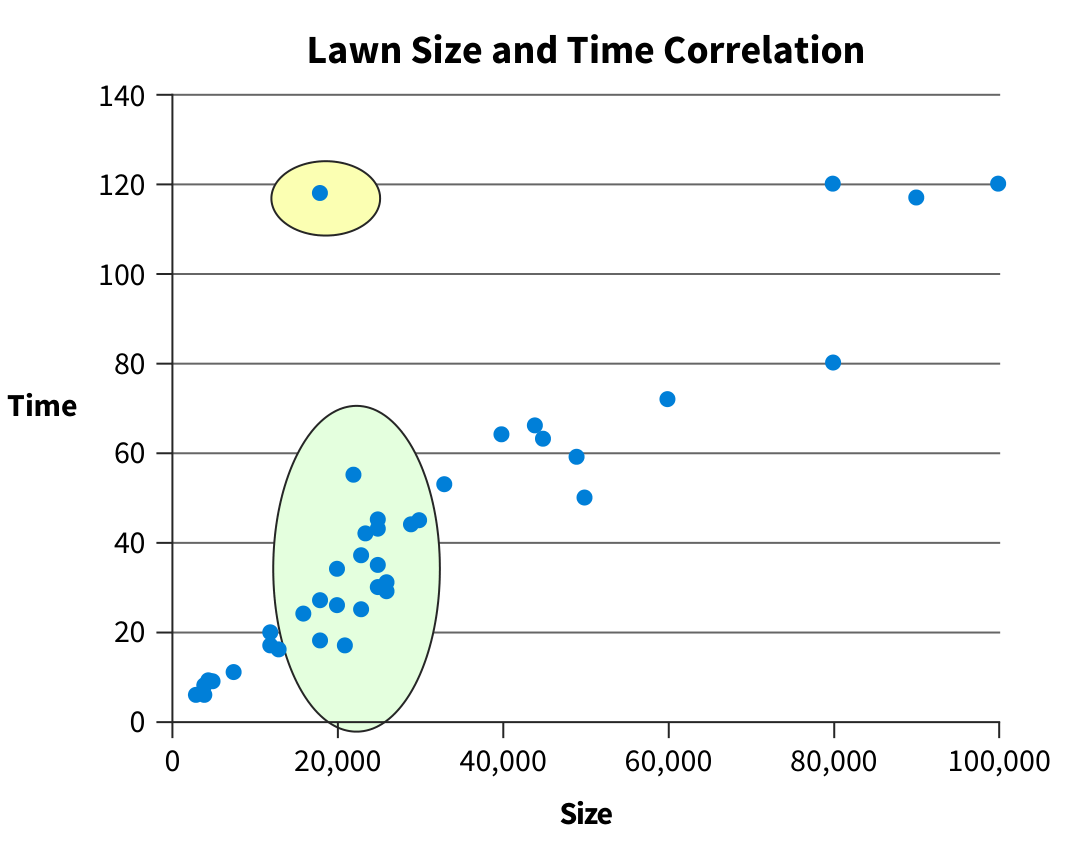
\includegraphics[width=0.95\textwidth,height=0.75\textheight,keepaspectratio]{../textbookForPractice/Figures/Ch_07/ILLUSTRATION 7.29.png}
    \end{figure}
\end{frame}

\begin{frame}{ILLUSTRATION 7.30}

    \begin{figure}[h]
        \centering
        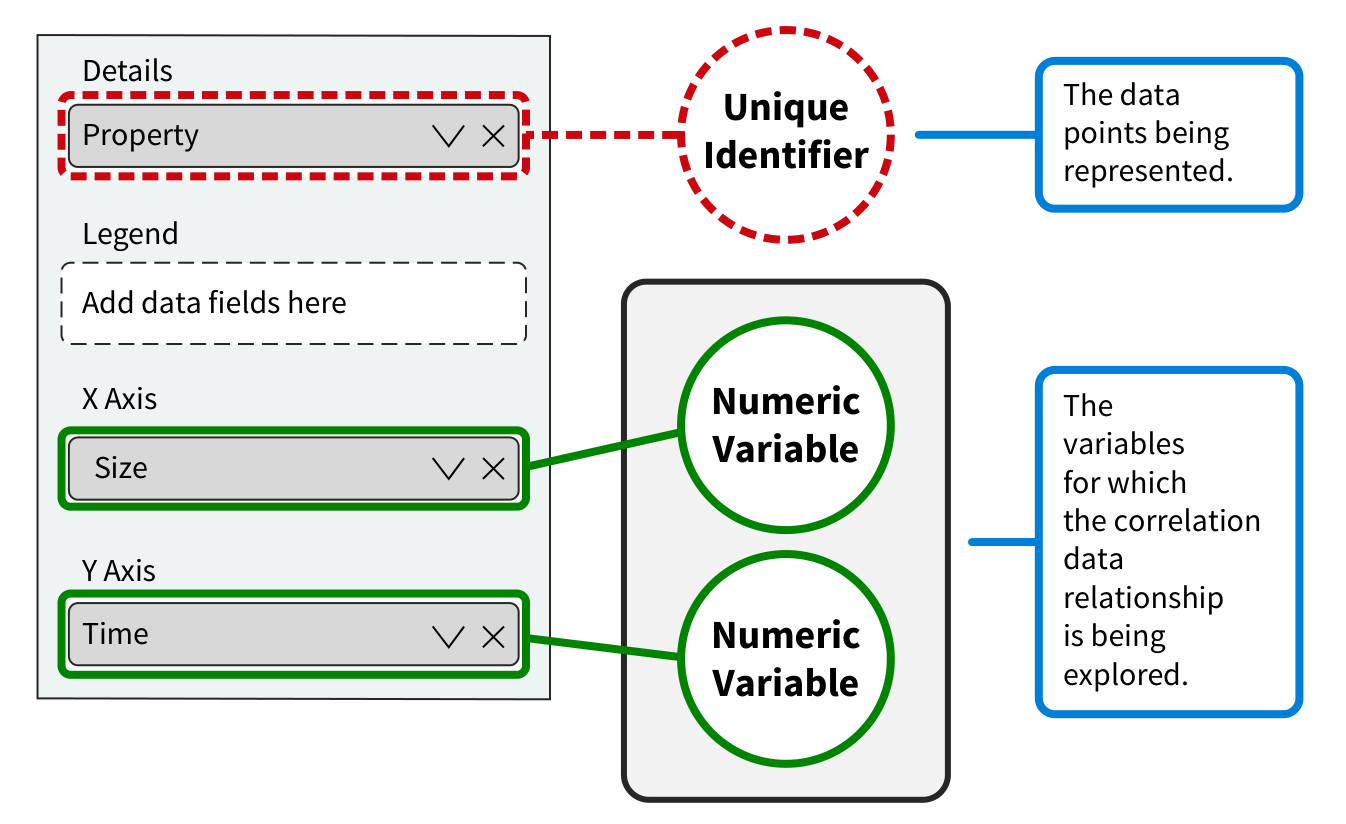
\includegraphics[width=0.95\textwidth,height=0.75\textheight,keepaspectratio]{../textbookForPractice/Figures/Ch_07/ILLUSTRATION 7.30.png}
    \end{figure}
\end{frame}

\begin{frame}{Nguyên tắc Thiết kế Biểu đồ}
\begin{itemize}
    \item \textbf{Giữ sự đơn giản (Keep it Simple):} Tránh lạm dụng 3D, bóng đổ hoặc màu sắc lòe loẹt gây xao nhãng (Chartjunk).
    \item \textbf{Rõ ràng (Clarity):} Trục tọa độ, nhãn dữ liệu (Data labels), và tiêu đề phải dễ đọc và mang tính mô tả.
    \item \textbf{Sử dụng Màu sắc có chủ ý:} Dùng màu đỏ cho sự giảm sút/rủi ro, màu xanh cho sự tăng trưởng.
\end{itemize}
\end{frame}

\begin{frame}{ILLUSTRATION 7.31}

    \begin{figure}[h]
        \centering
        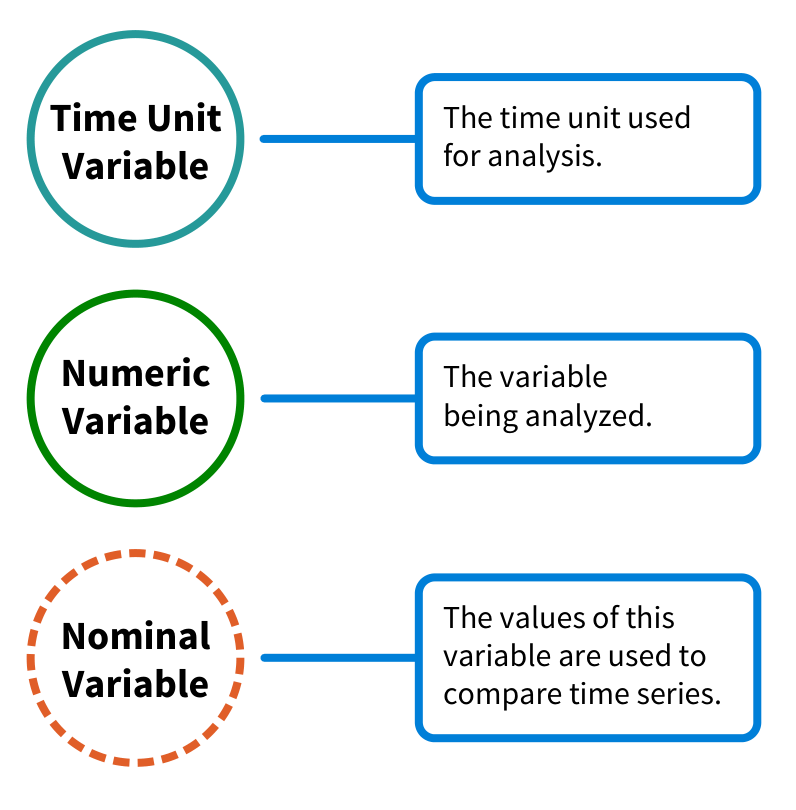
\includegraphics[width=0.95\textwidth,height=0.75\textheight,keepaspectratio]{../textbookForPractice/Figures/Ch_07/ILLUSTRATION 7.31.png}
    \end{figure}
\end{frame}

\begin{frame}{ILLUSTRATION 7.32}

    \begin{figure}[h]
        \centering
        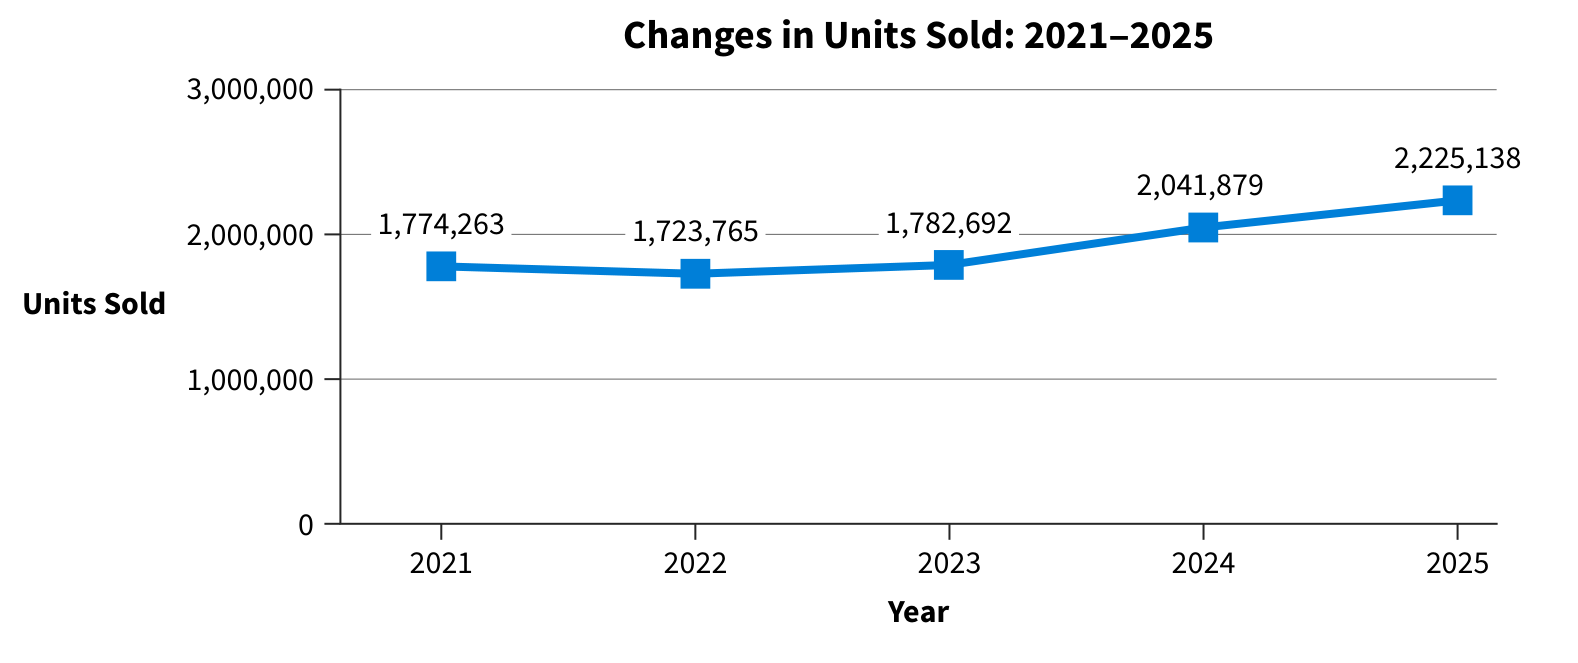
\includegraphics[width=0.95\textwidth,height=0.75\textheight,keepaspectratio]{../textbookForPractice/Figures/Ch_07/ILLUSTRATION 7.32.png}
    \end{figure}
\end{frame}

\begin{frame}{ILLUSTRATION 7.33}

    \begin{figure}[h]
        \centering
        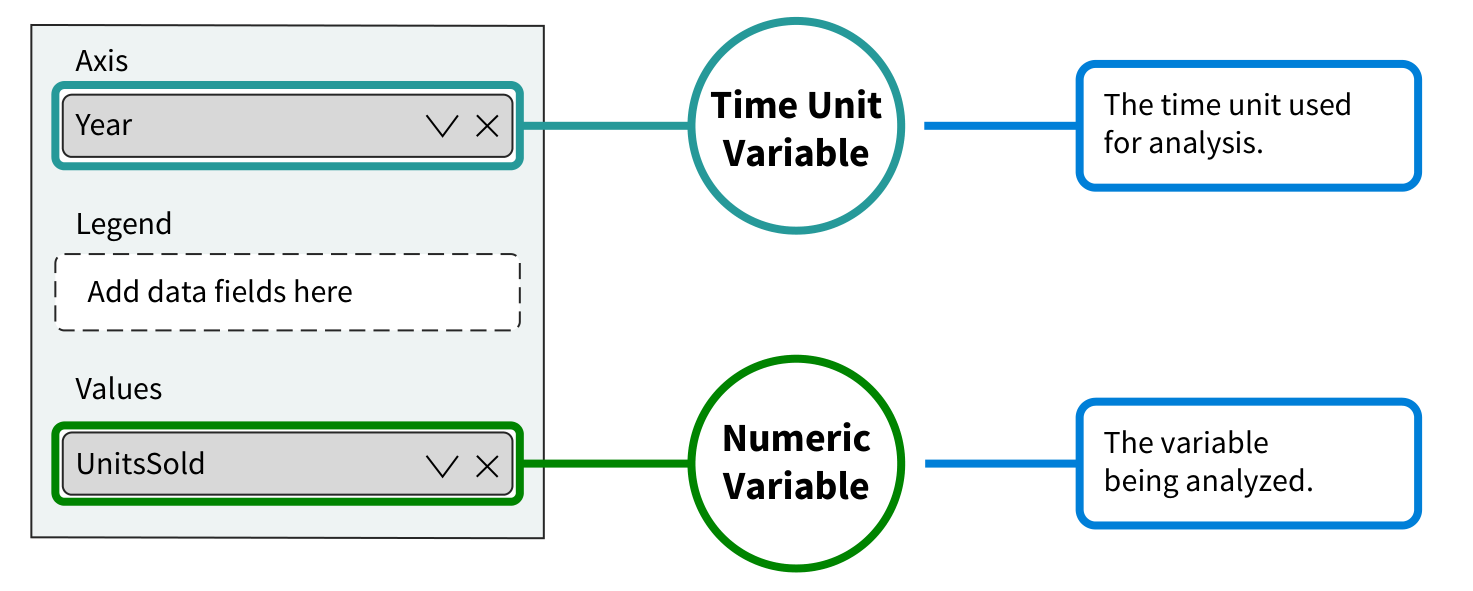
\includegraphics[width=0.95\textwidth,height=0.75\textheight,keepaspectratio]{../textbookForPractice/Figures/Ch_07/ILLUSTRATION 7.33.png}
    \end{figure}
\end{frame}

\begin{frame}{ILLUSTRATION 7.34}

    \begin{figure}[h]
        \centering
        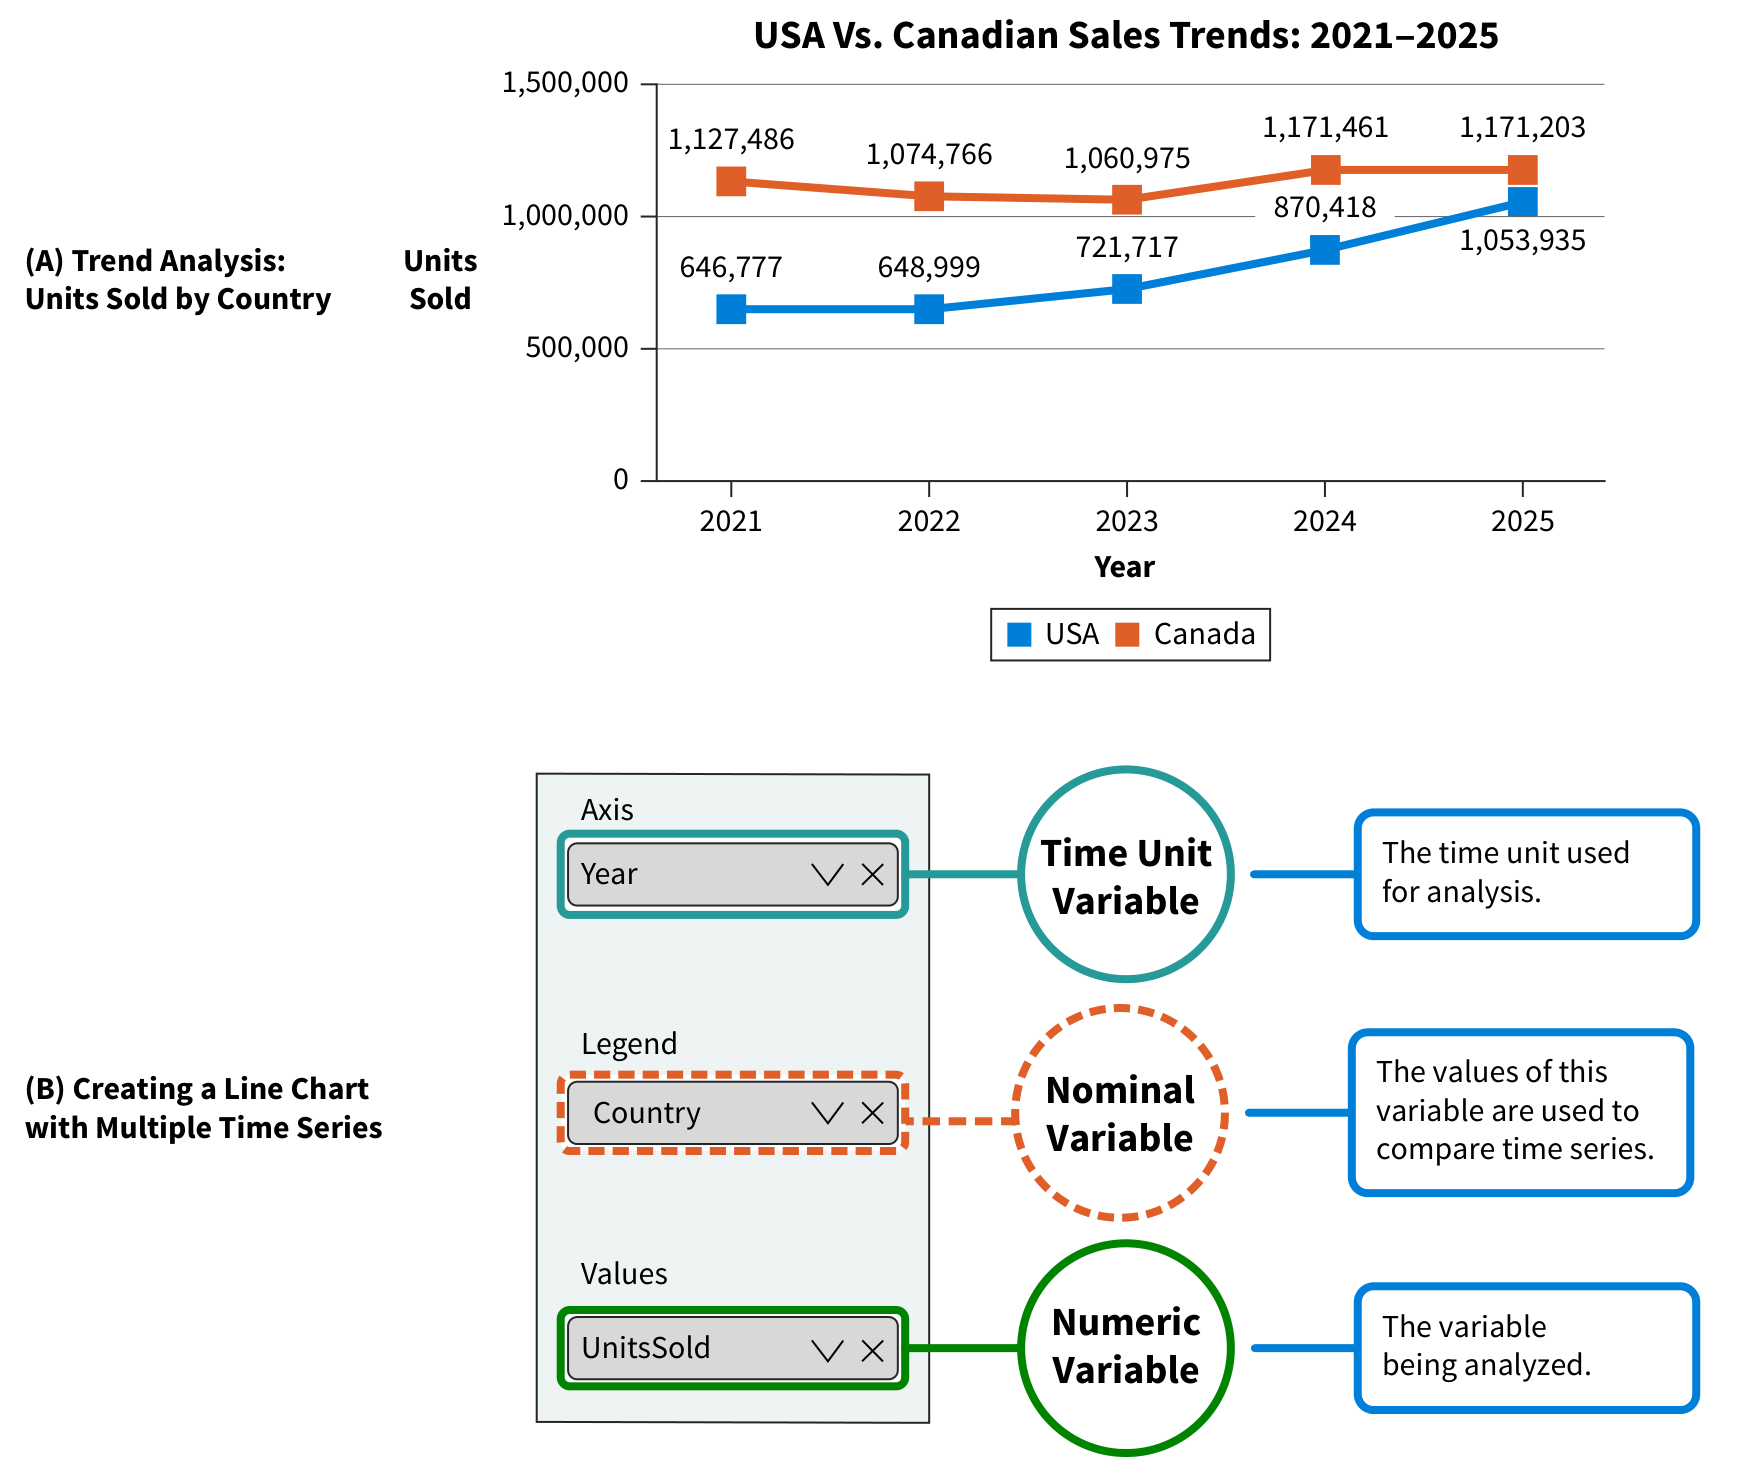
\includegraphics[width=0.95\textwidth,height=0.75\textheight,keepaspectratio]{../textbookForPractice/Figures/Ch_07/ILLUSTRATION 7.34.png}
    \end{figure}
\end{frame}

\begin{frame}{7.3 Khám phá Dữ liệu Đa chiều (Tích hợp)}
\begin{itemize}
    \item \textbf{Tích hợp Mối quan hệ:} Sử dụng kết hợp nhiều loại biểu đồ để có cái nhìn toàn diện hơn (Holistic view).
    \item \textbf{Hai mẫu trong một (Single Visualization):}
    \begin{itemize}
        \item Biểu đồ Đa trục (Dual-axis): So sánh hai chỉ số có thang đo khác nhau trên cùng một biểu đồ (ví dụ: Doanh thu - Cột, Tỷ suất LN - Đường).
        \item Biểu đồ Bong bóng (Bubble chart): Thể hiện 3 biến dữ liệu (Trục X, Trục Y, Độ lớn bong bóng).
    \end{itemize}
\end{itemize}
\end{frame}

\begin{frame}{ILLUSTRATION 7.35}

    \begin{figure}[h]
        \centering
        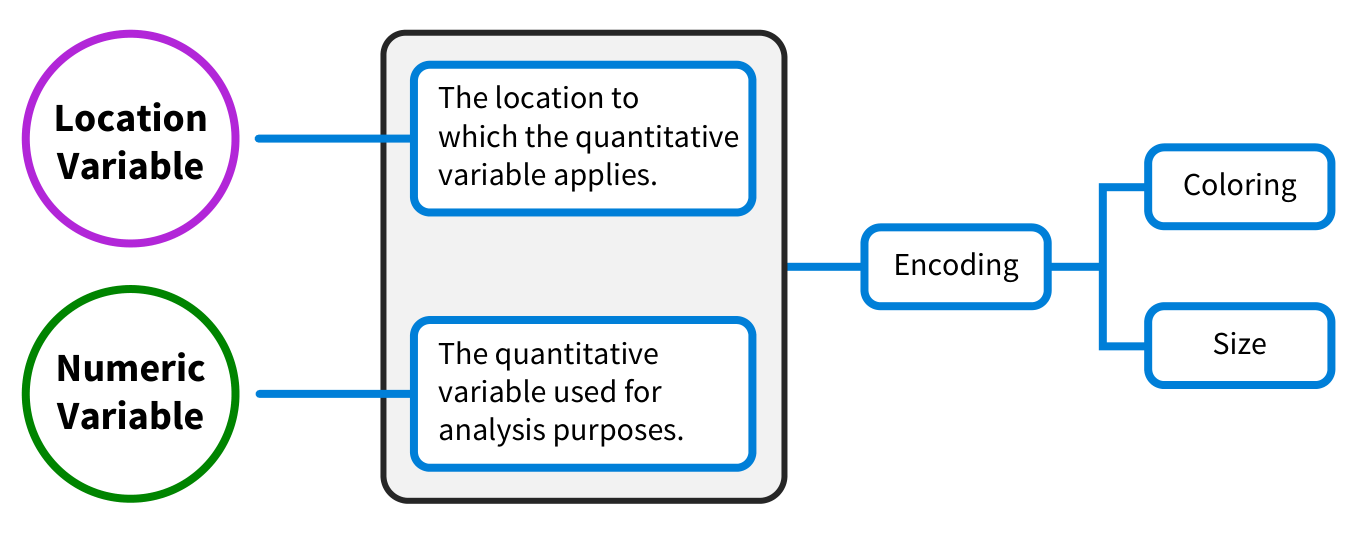
\includegraphics[width=0.95\textwidth,height=0.75\textheight,keepaspectratio]{../textbookForPractice/Figures/Ch_07/ILLUSTRATION 7.35.png}
    \end{figure}
\end{frame}

\begin{frame}{ILLUSTRATION 7.36}

    \begin{figure}[h]
        \centering
        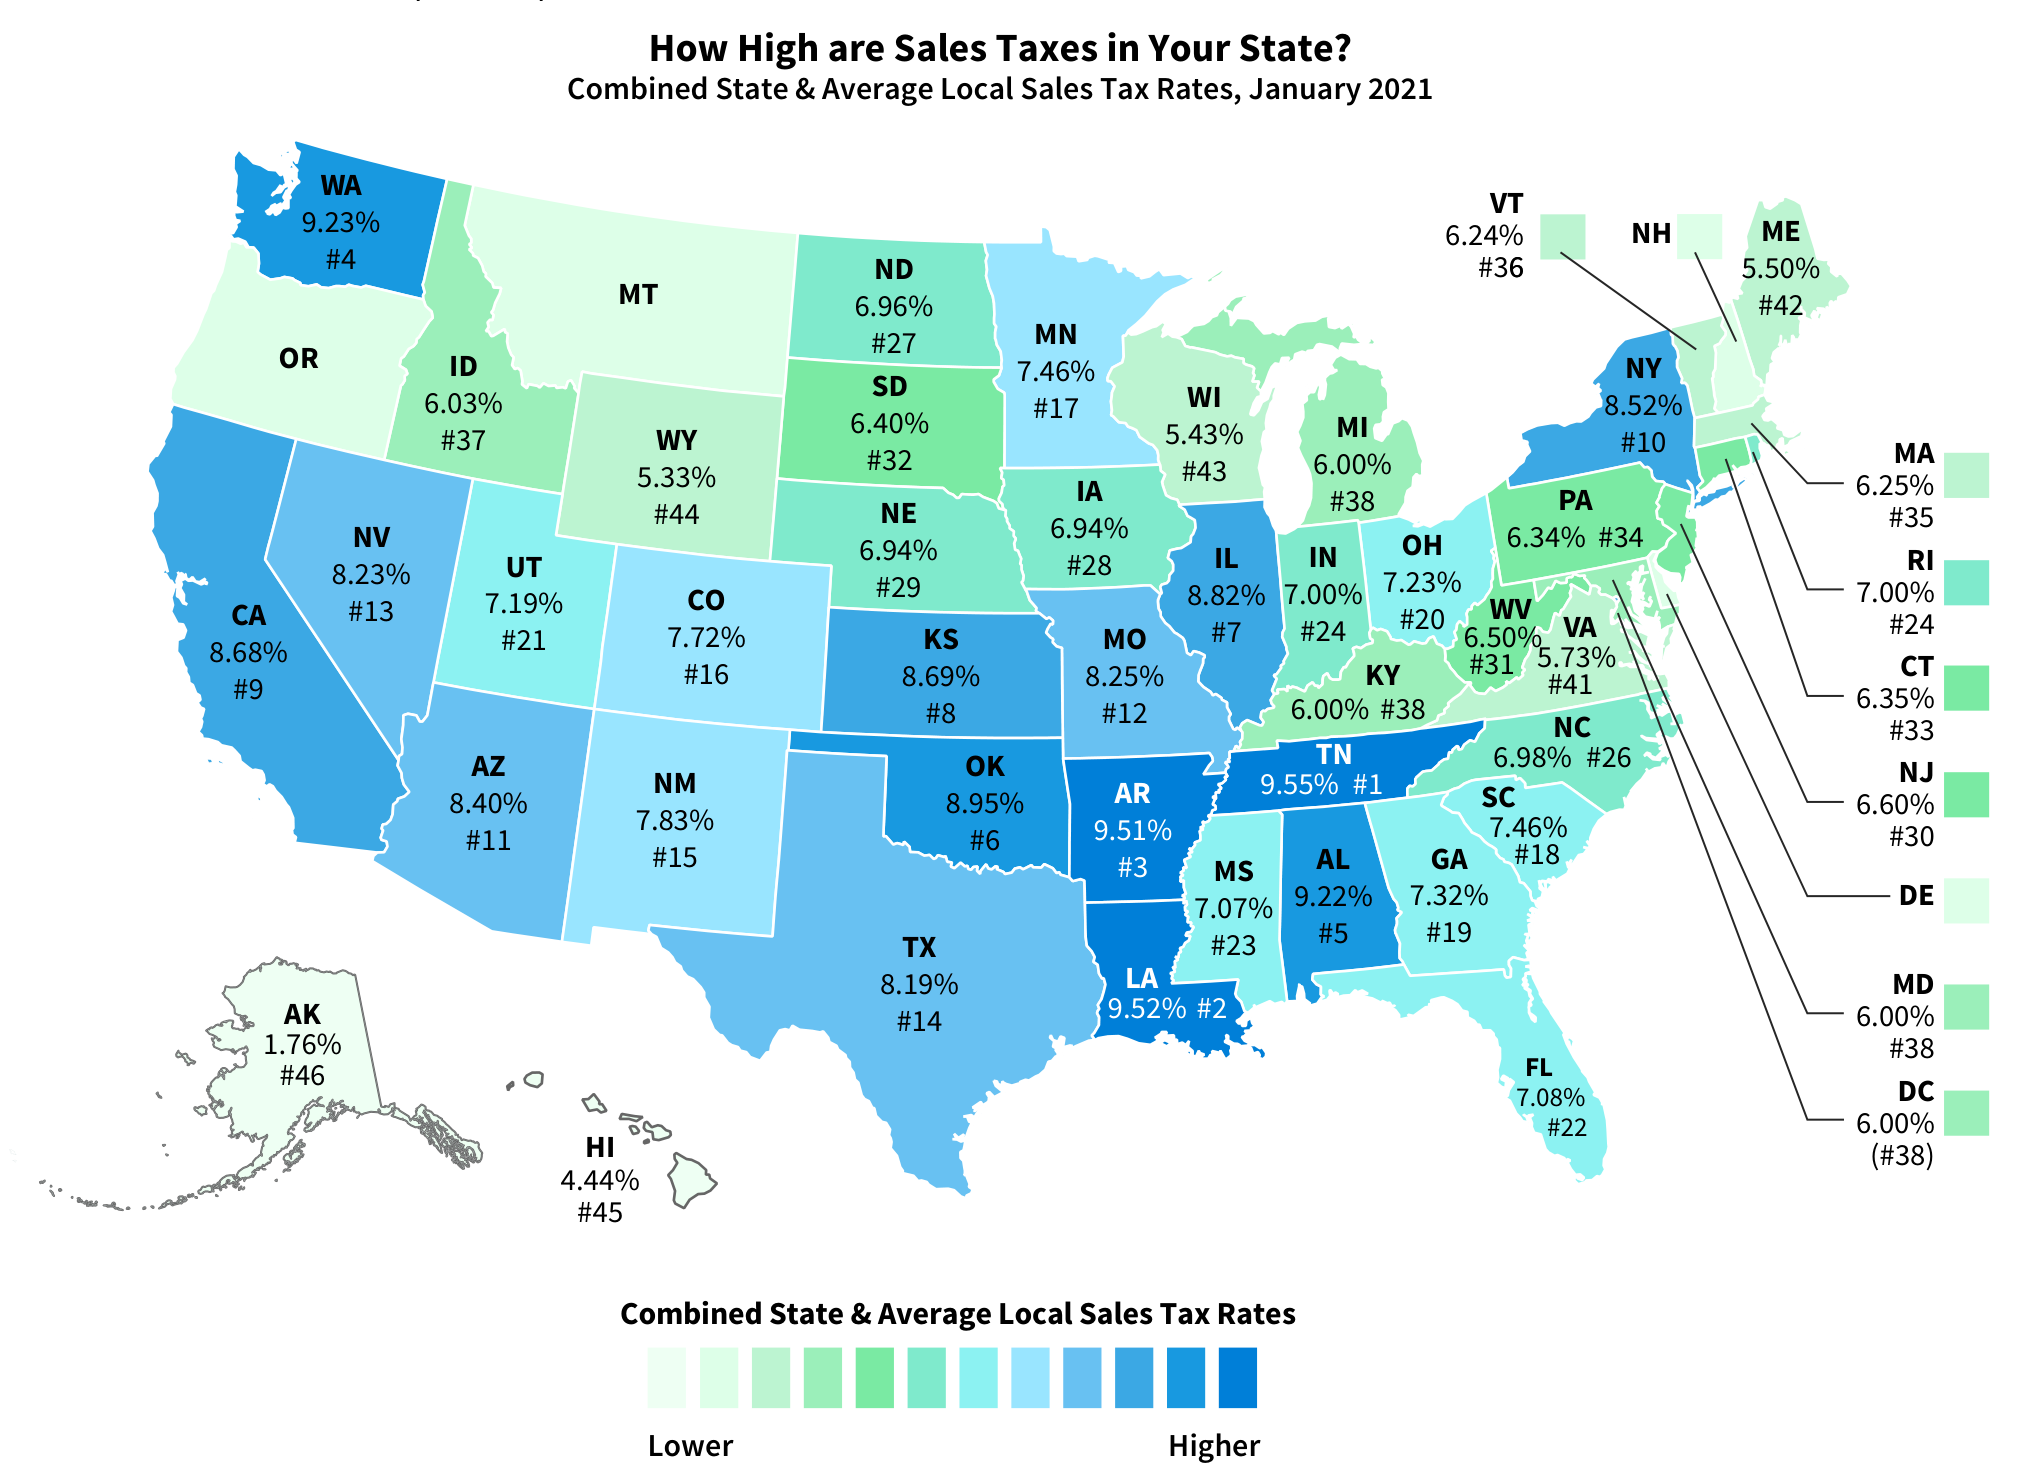
\includegraphics[width=0.95\textwidth,height=0.75\textheight,keepaspectratio]{../textbookForPractice/Figures/Ch_07/ILLUSTRATION 7.36.png}
    \end{figure}
\end{frame}

\begin{frame}{ILLUSTRATION 7.37}

    \begin{figure}[h]
        \centering
        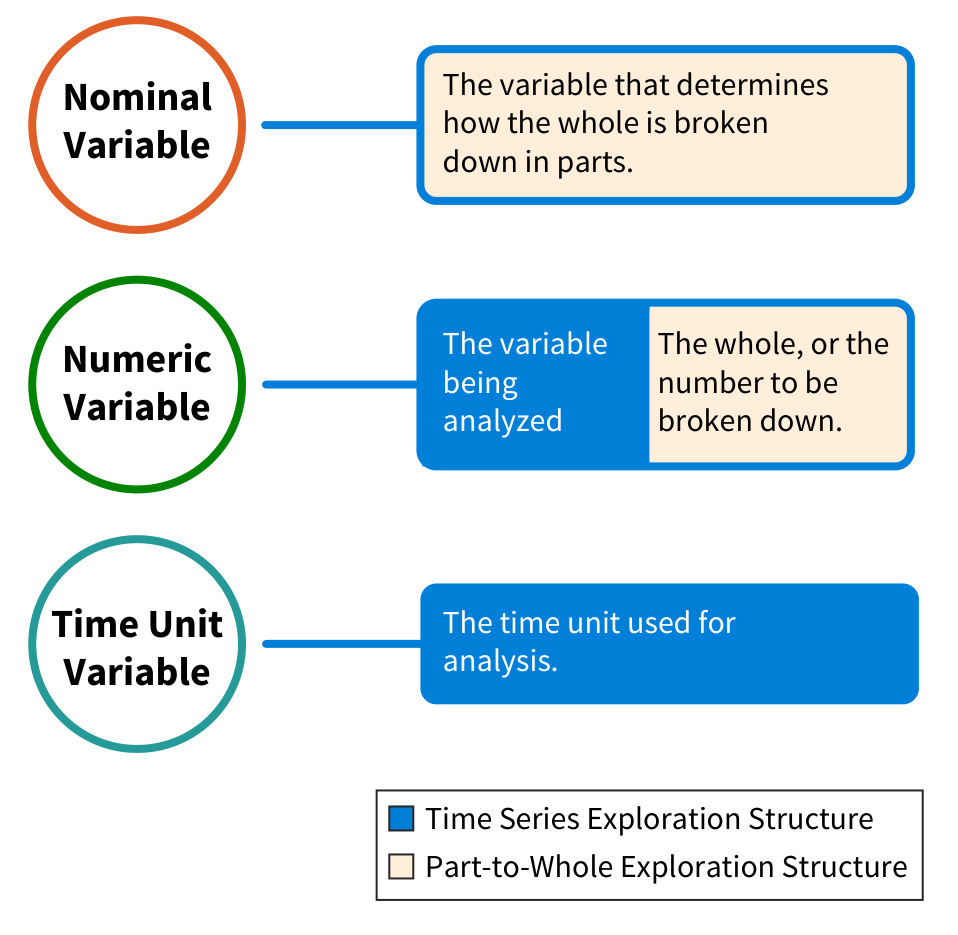
\includegraphics[width=0.95\textwidth,height=0.75\textheight,keepaspectratio]{../textbookForPractice/Figures/Ch_07/ILLUSTRATION 7.37.png}
    \end{figure}
\end{frame}

\begin{frame}{ILLUSTRATION 7.38}

    \begin{figure}[h]
        \centering
        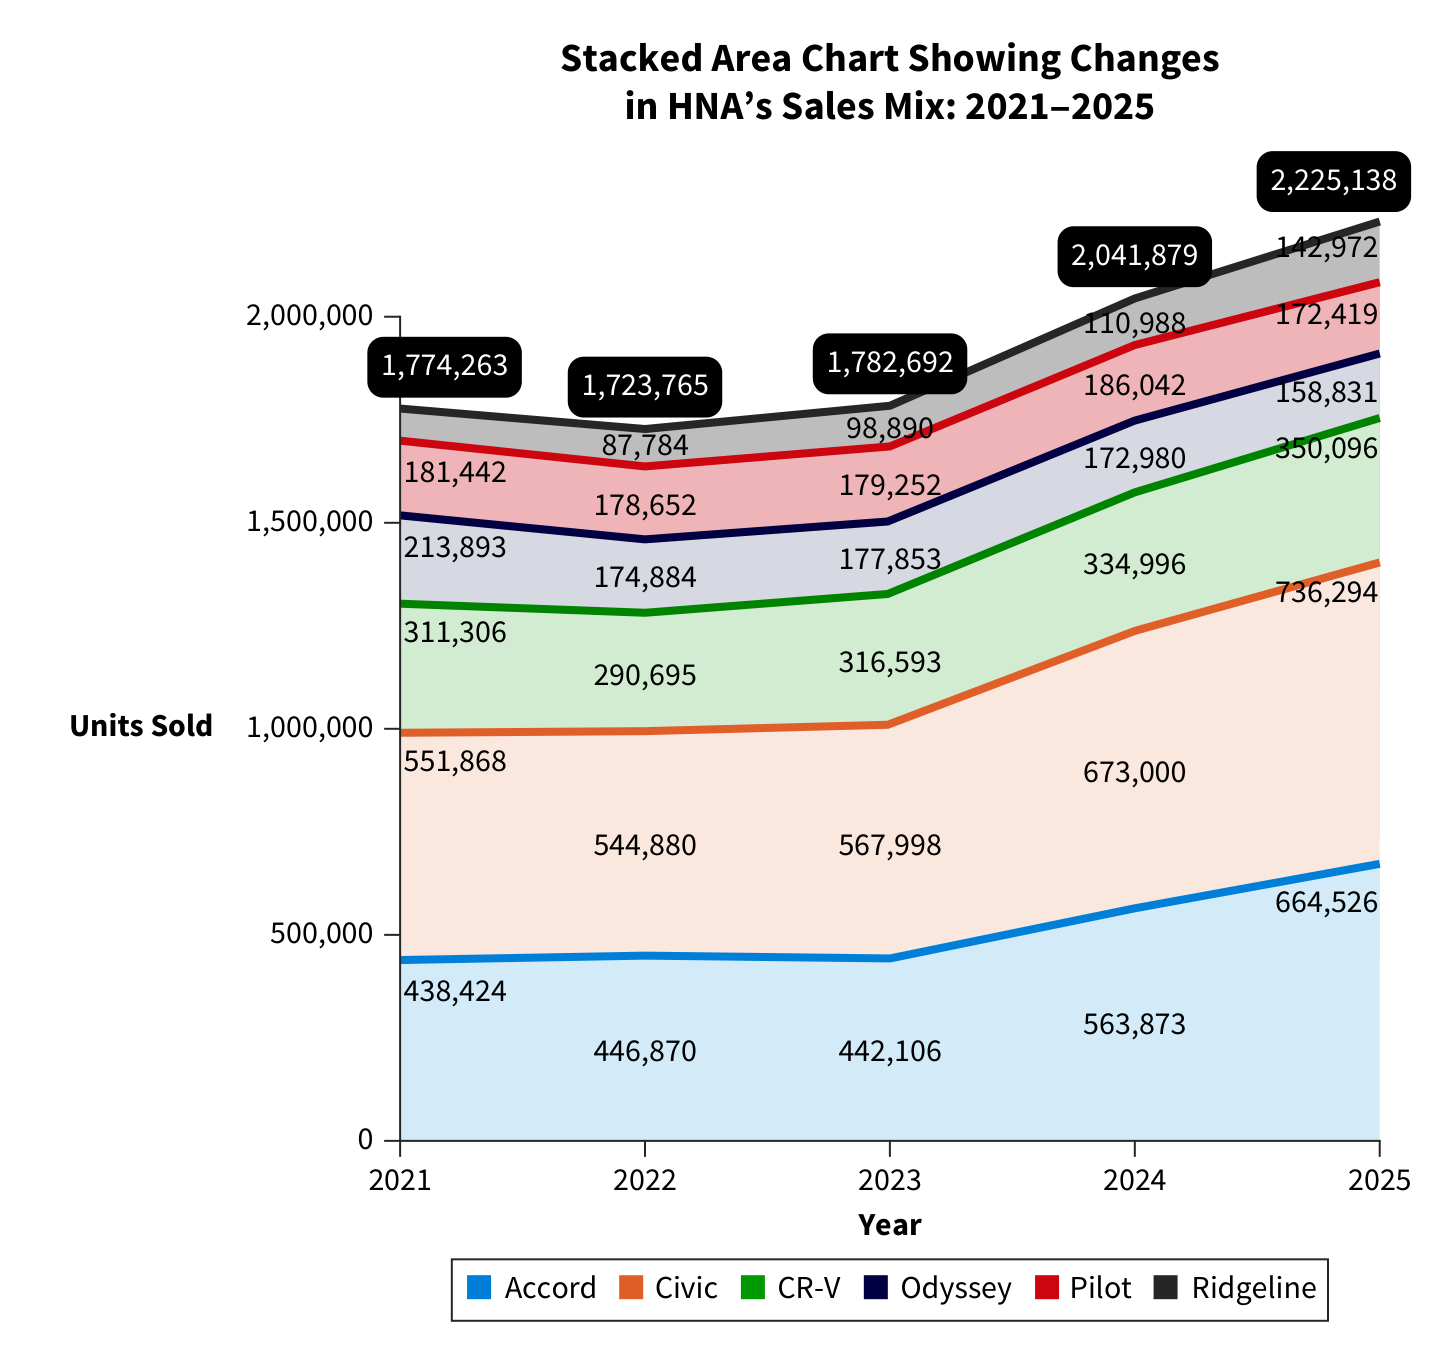
\includegraphics[width=0.95\textwidth,height=0.75\textheight,keepaspectratio]{../textbookForPractice/Figures/Ch_07/ILLUSTRATION 7.38.png}
    \end{figure}
\end{frame}

\begin{frame}{ILLUSTRATION 7.39}

    \begin{figure}[h]
        \centering
        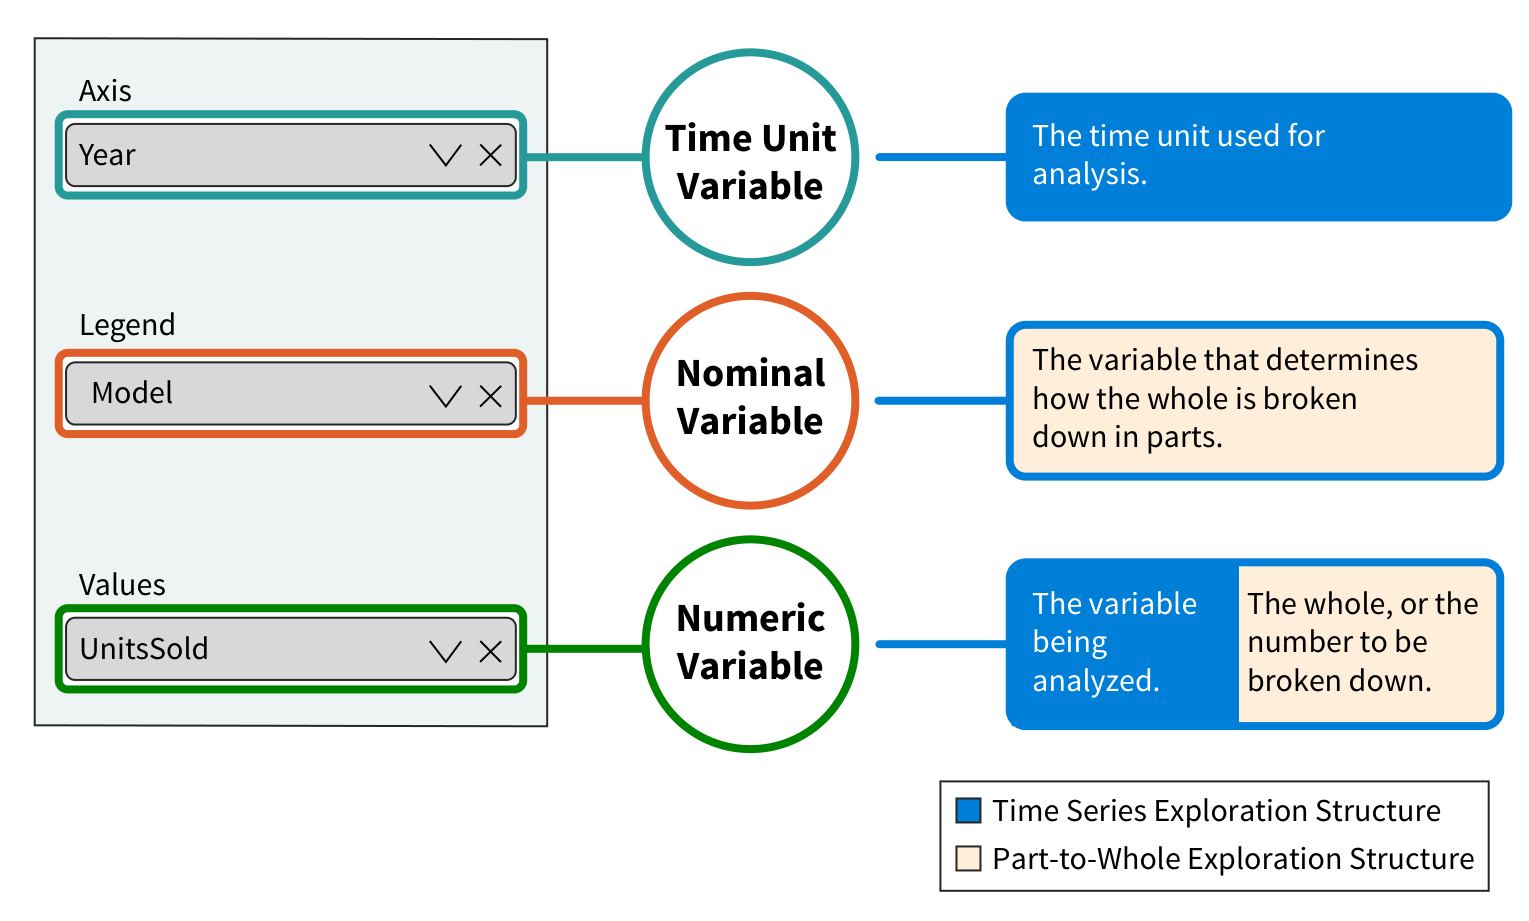
\includegraphics[width=0.95\textwidth,height=0.75\textheight,keepaspectratio]{../textbookForPractice/Figures/Ch_07/ILLUSTRATION 7.39.png}
    \end{figure}
\end{frame}

\begin{frame}{ILLUSTRATION 7.40}

    \begin{figure}[h]
        \centering
        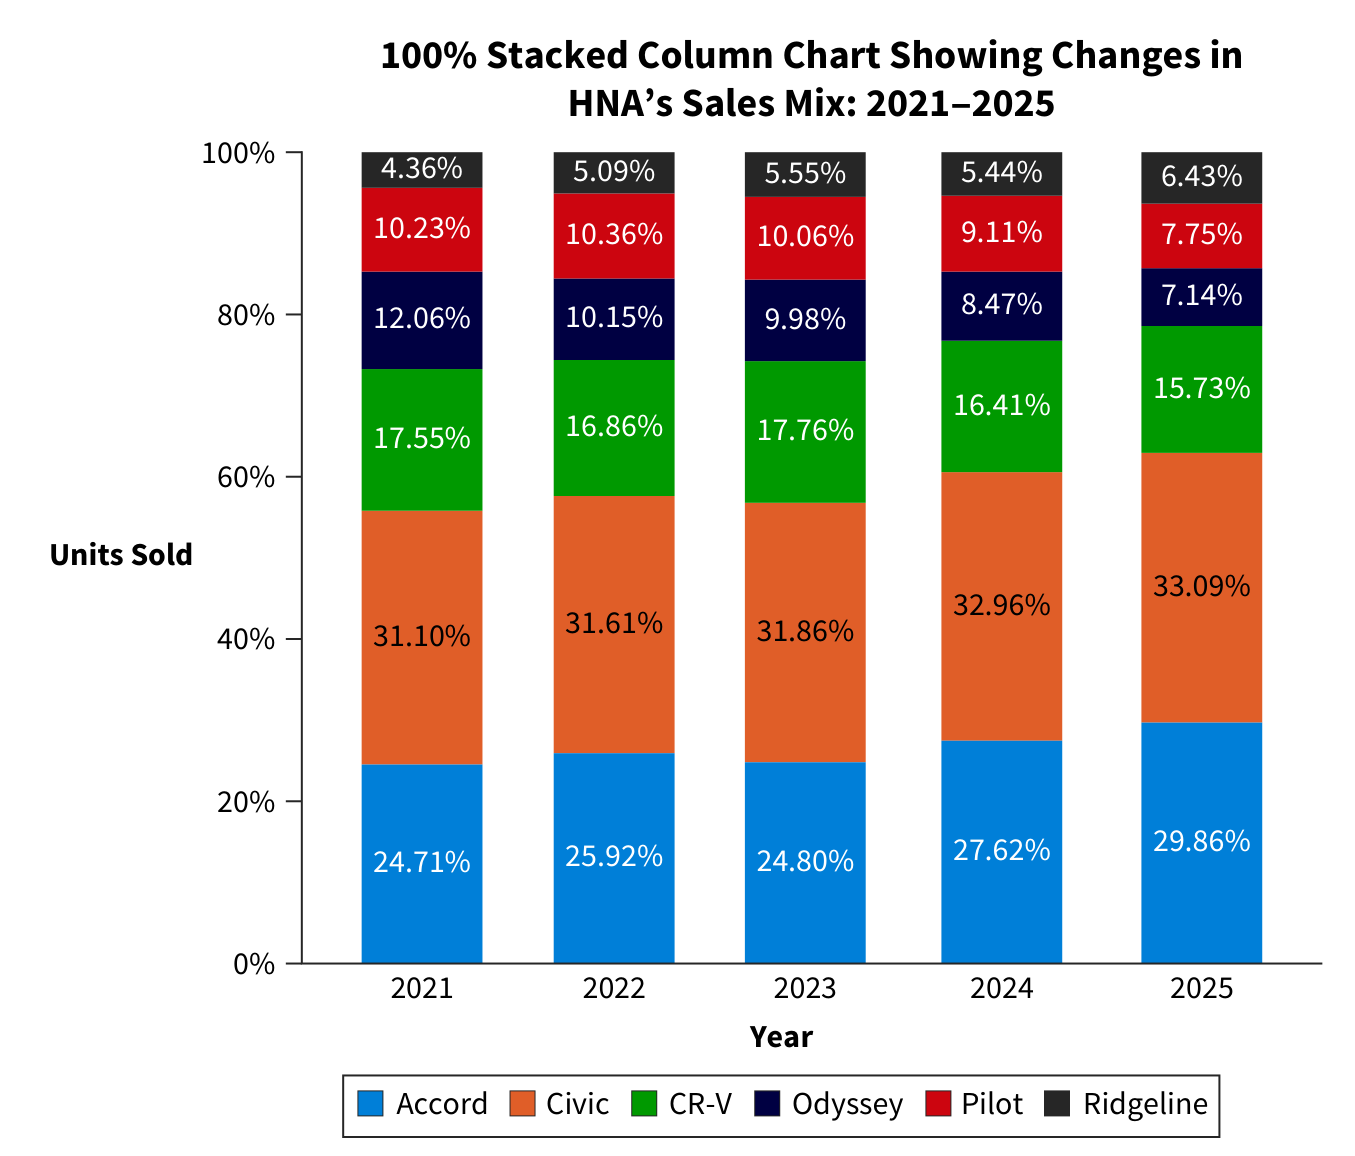
\includegraphics[width=0.95\textwidth,height=0.75\textheight,keepaspectratio]{../textbookForPractice/Figures/Ch_07/ILLUSTRATION 7.40.png}
    \end{figure}
\end{frame}

\begin{frame}{ILLUSTRATION 7.41}

    \begin{figure}[h]
        \centering
        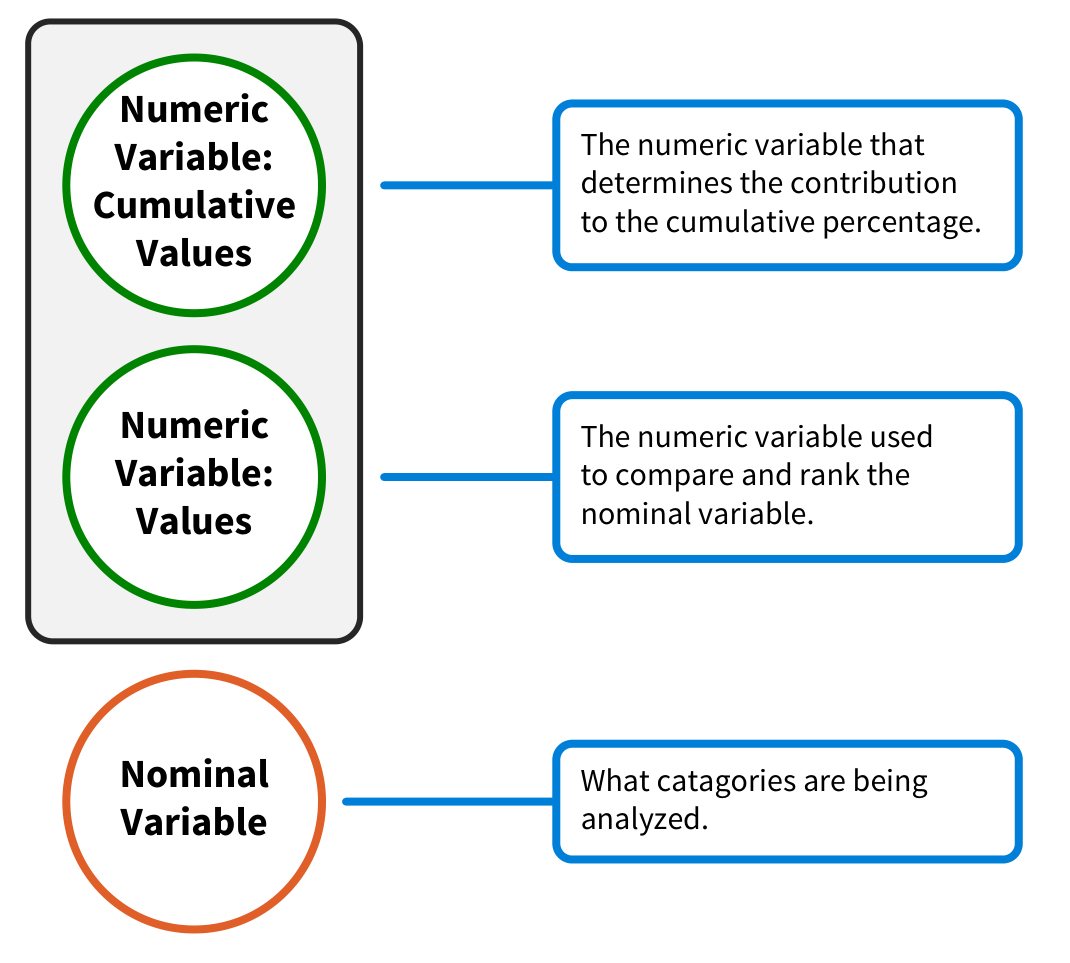
\includegraphics[width=0.95\textwidth,height=0.75\textheight,keepaspectratio]{../textbookForPractice/Figures/Ch_07/ILLUSTRATION 7.41.png}
    \end{figure}
\end{frame}

\begin{frame}{ILLUSTRATION 7.42}

    \begin{figure}[h]
        \centering
        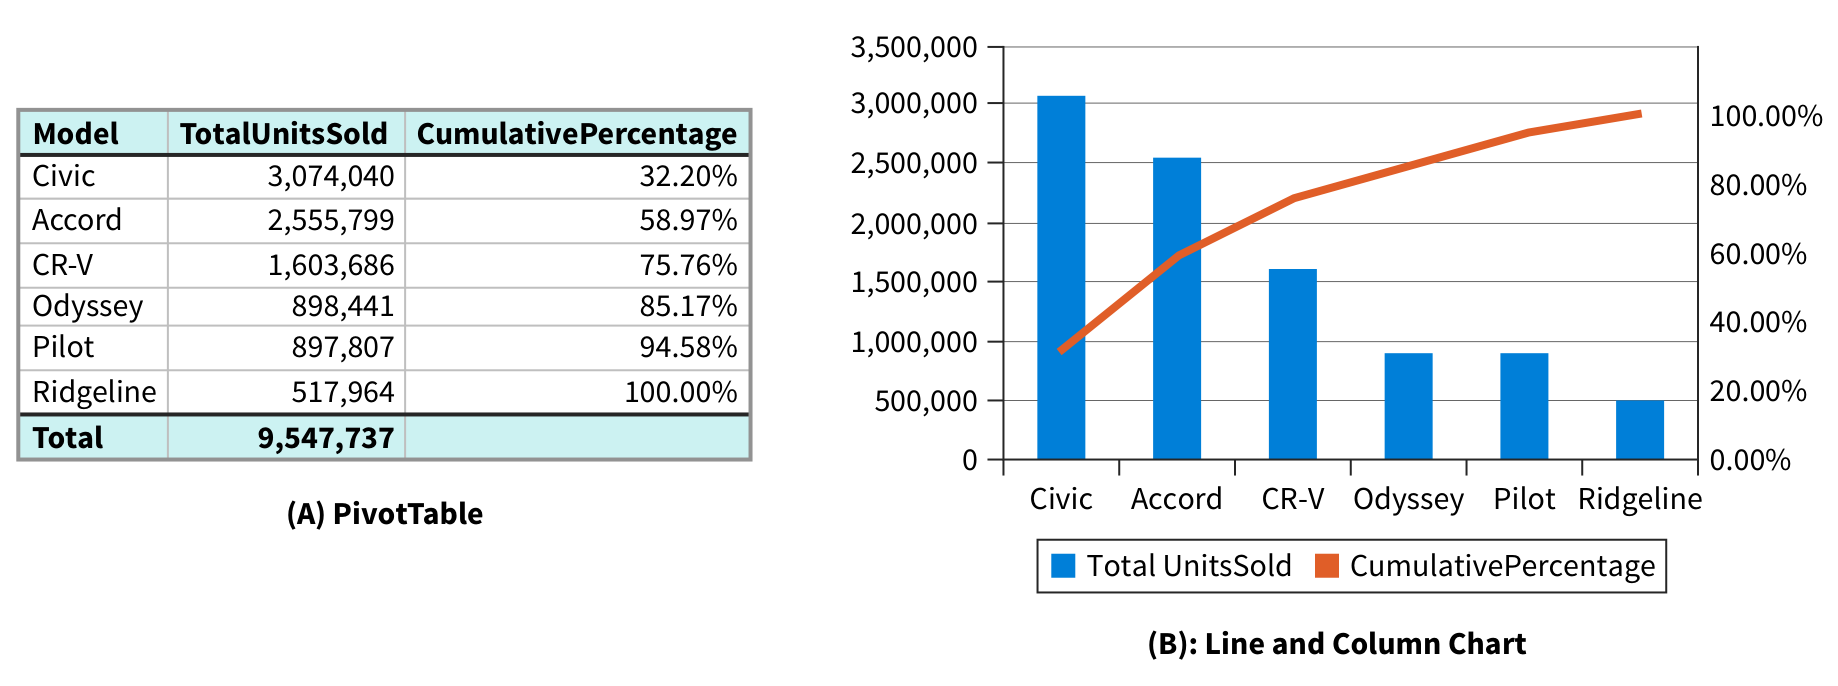
\includegraphics[width=0.95\textwidth,height=0.75\textheight,keepaspectratio]{../textbookForPractice/Figures/Ch_07/ILLUSTRATION 7.42.png}
    \end{figure}
\end{frame}

\begin{frame}{ILLUSTRATION 7.43}

    \begin{figure}[h]
        \centering
        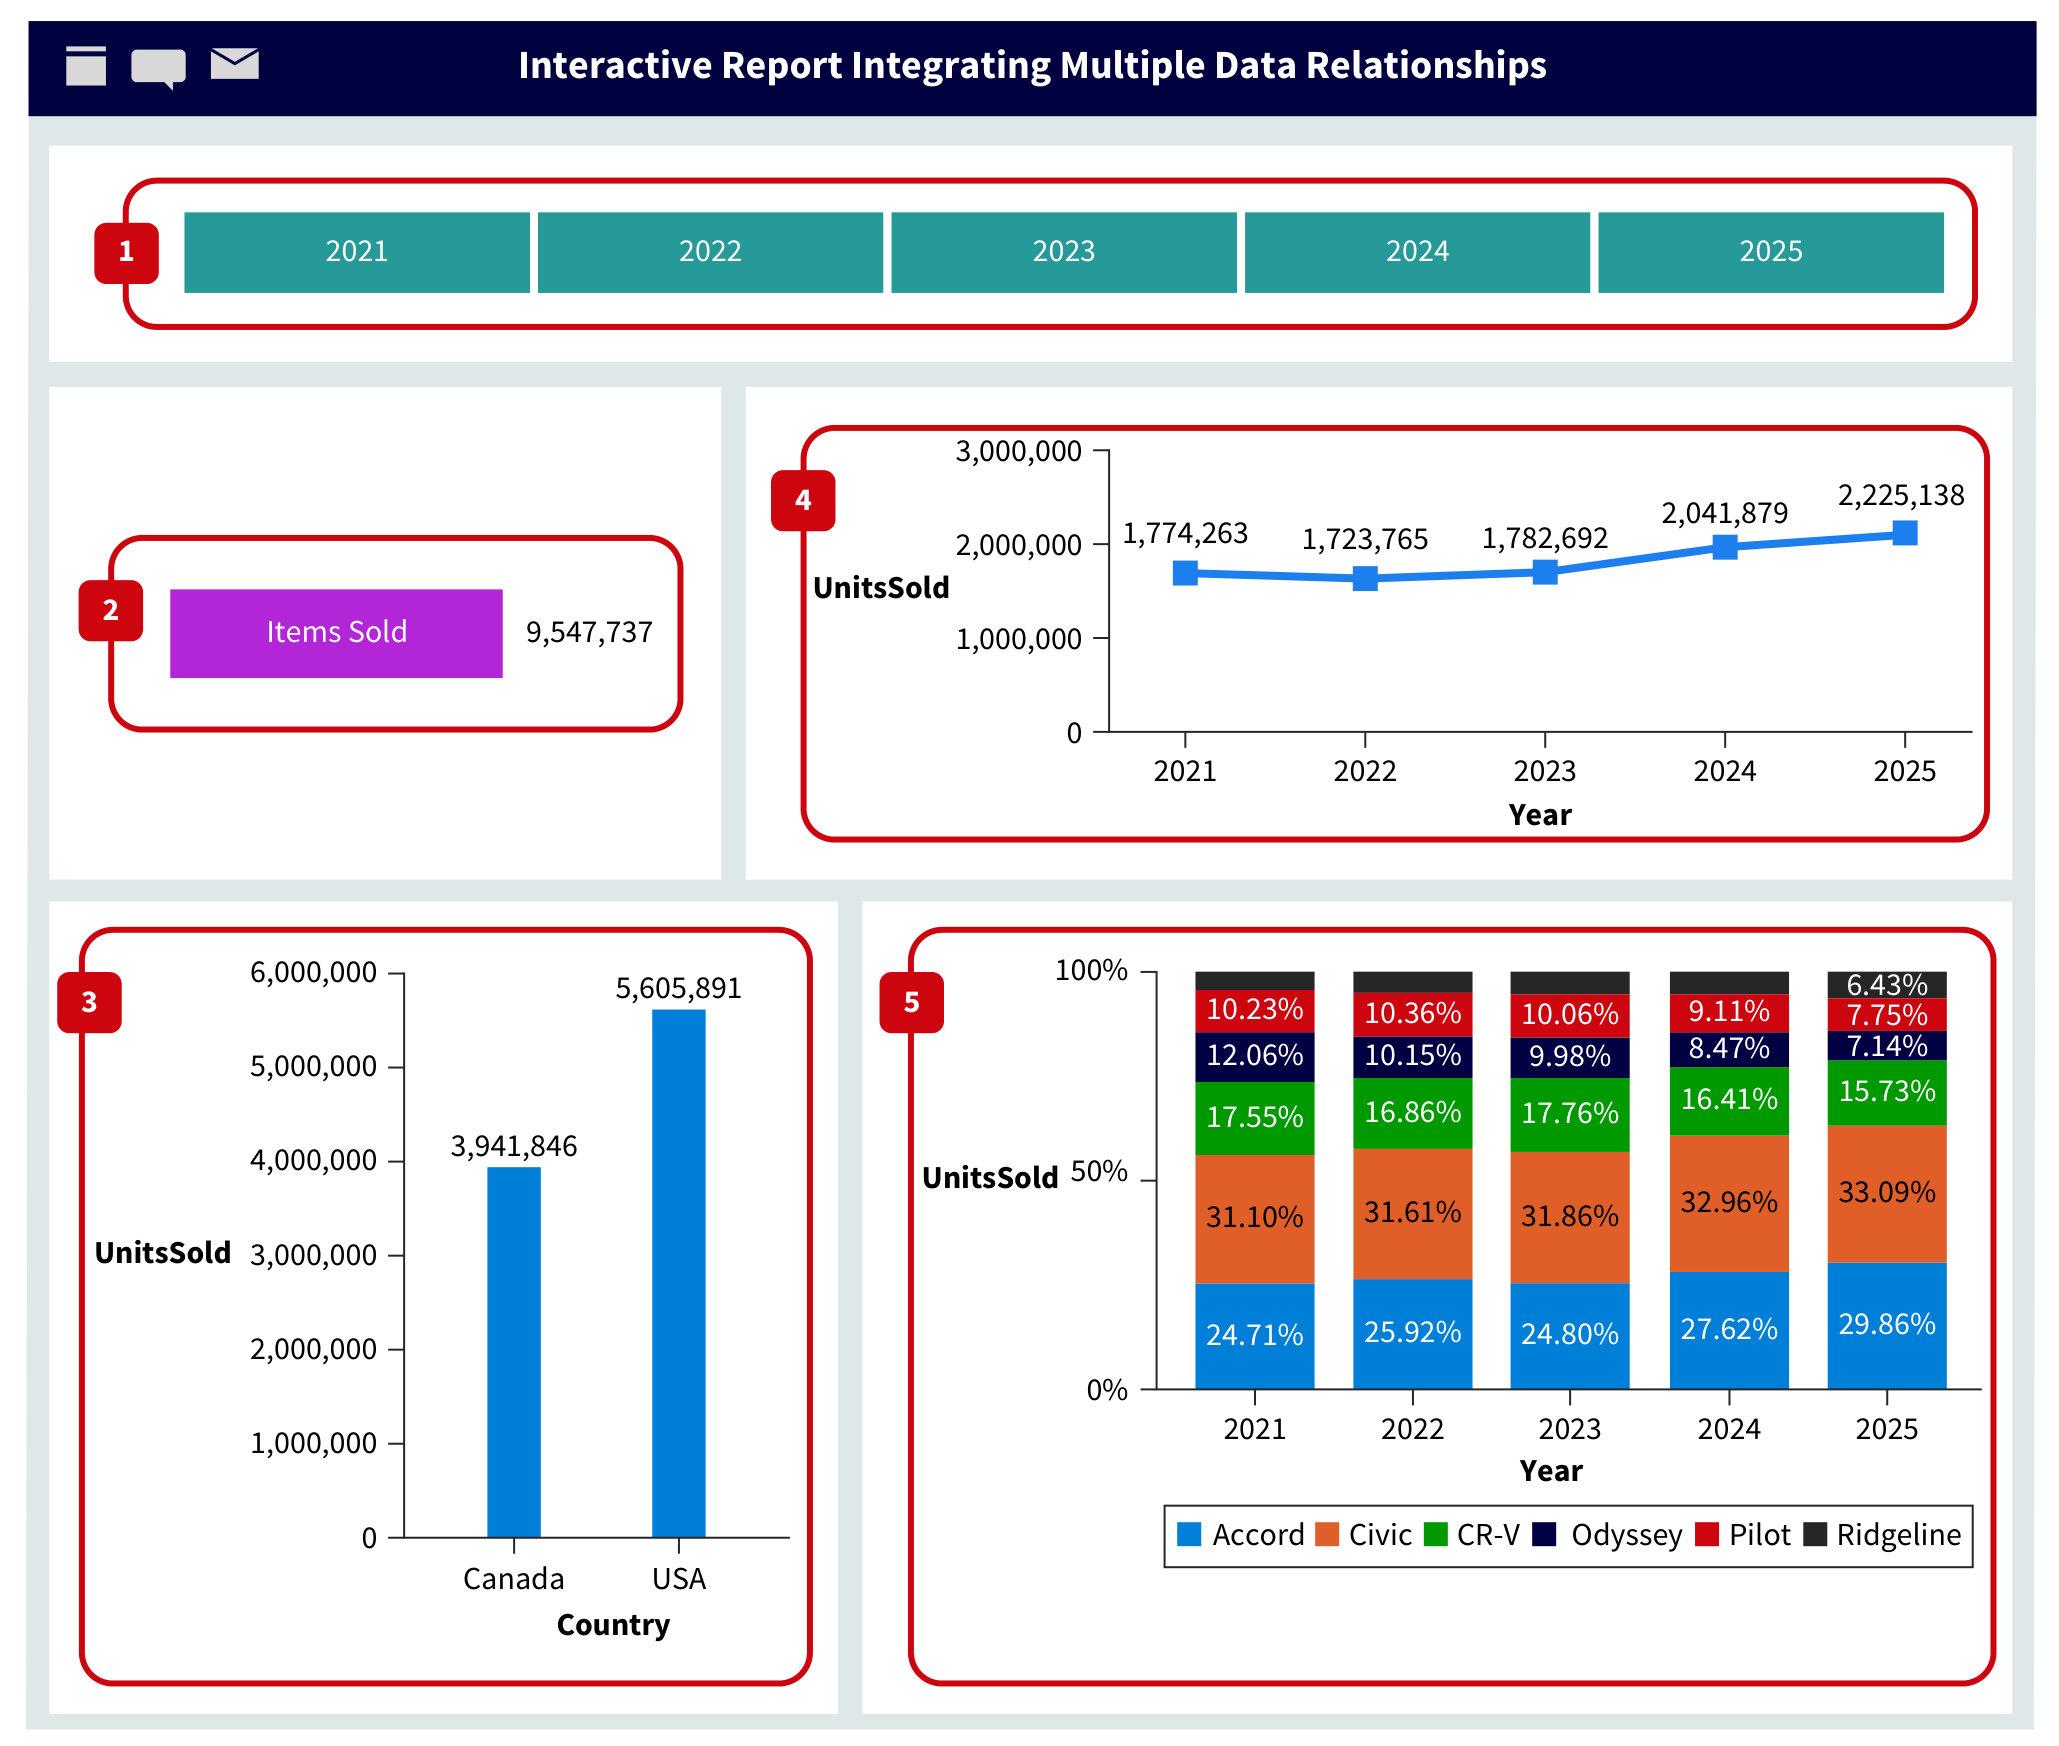
\includegraphics[width=0.95\textwidth,height=0.75\textheight,keepaspectratio]{../textbookForPractice/Figures/Ch_07/ILLUSTRATION 7.43.png}
    \end{figure}
\end{frame}

\begin{frame}{Bảng điều khiển (Dashboards)}
\begin{itemize}
    \item \textbf{Dashboard là gì?} Là giao diện trực quan tổng hợp nhiều biểu đồ, chỉ số quan trọng (KPIs) trên cùng một màn hình.
    \item \textbf{Tính Tương tác (Interactivity):} Người dùng có thể click, lọc (Slicers), khoan sâu (Drill-down) để khám phá chi tiết (Ví dụ: Từ doanh thu Tổng Công ty khoan xuống từng Chi nhánh).
    \item \textbf{Giá trị Kế toán:} Giúp Ban Lãnh đạo ra quyết định nhanh chóng, dựa trên dữ liệu (Data-driven decision making).
\end{itemize}
\end{frame}

\begin{frame}{ILLUSTRATION 7.44}

    \begin{figure}[h]
        \centering
        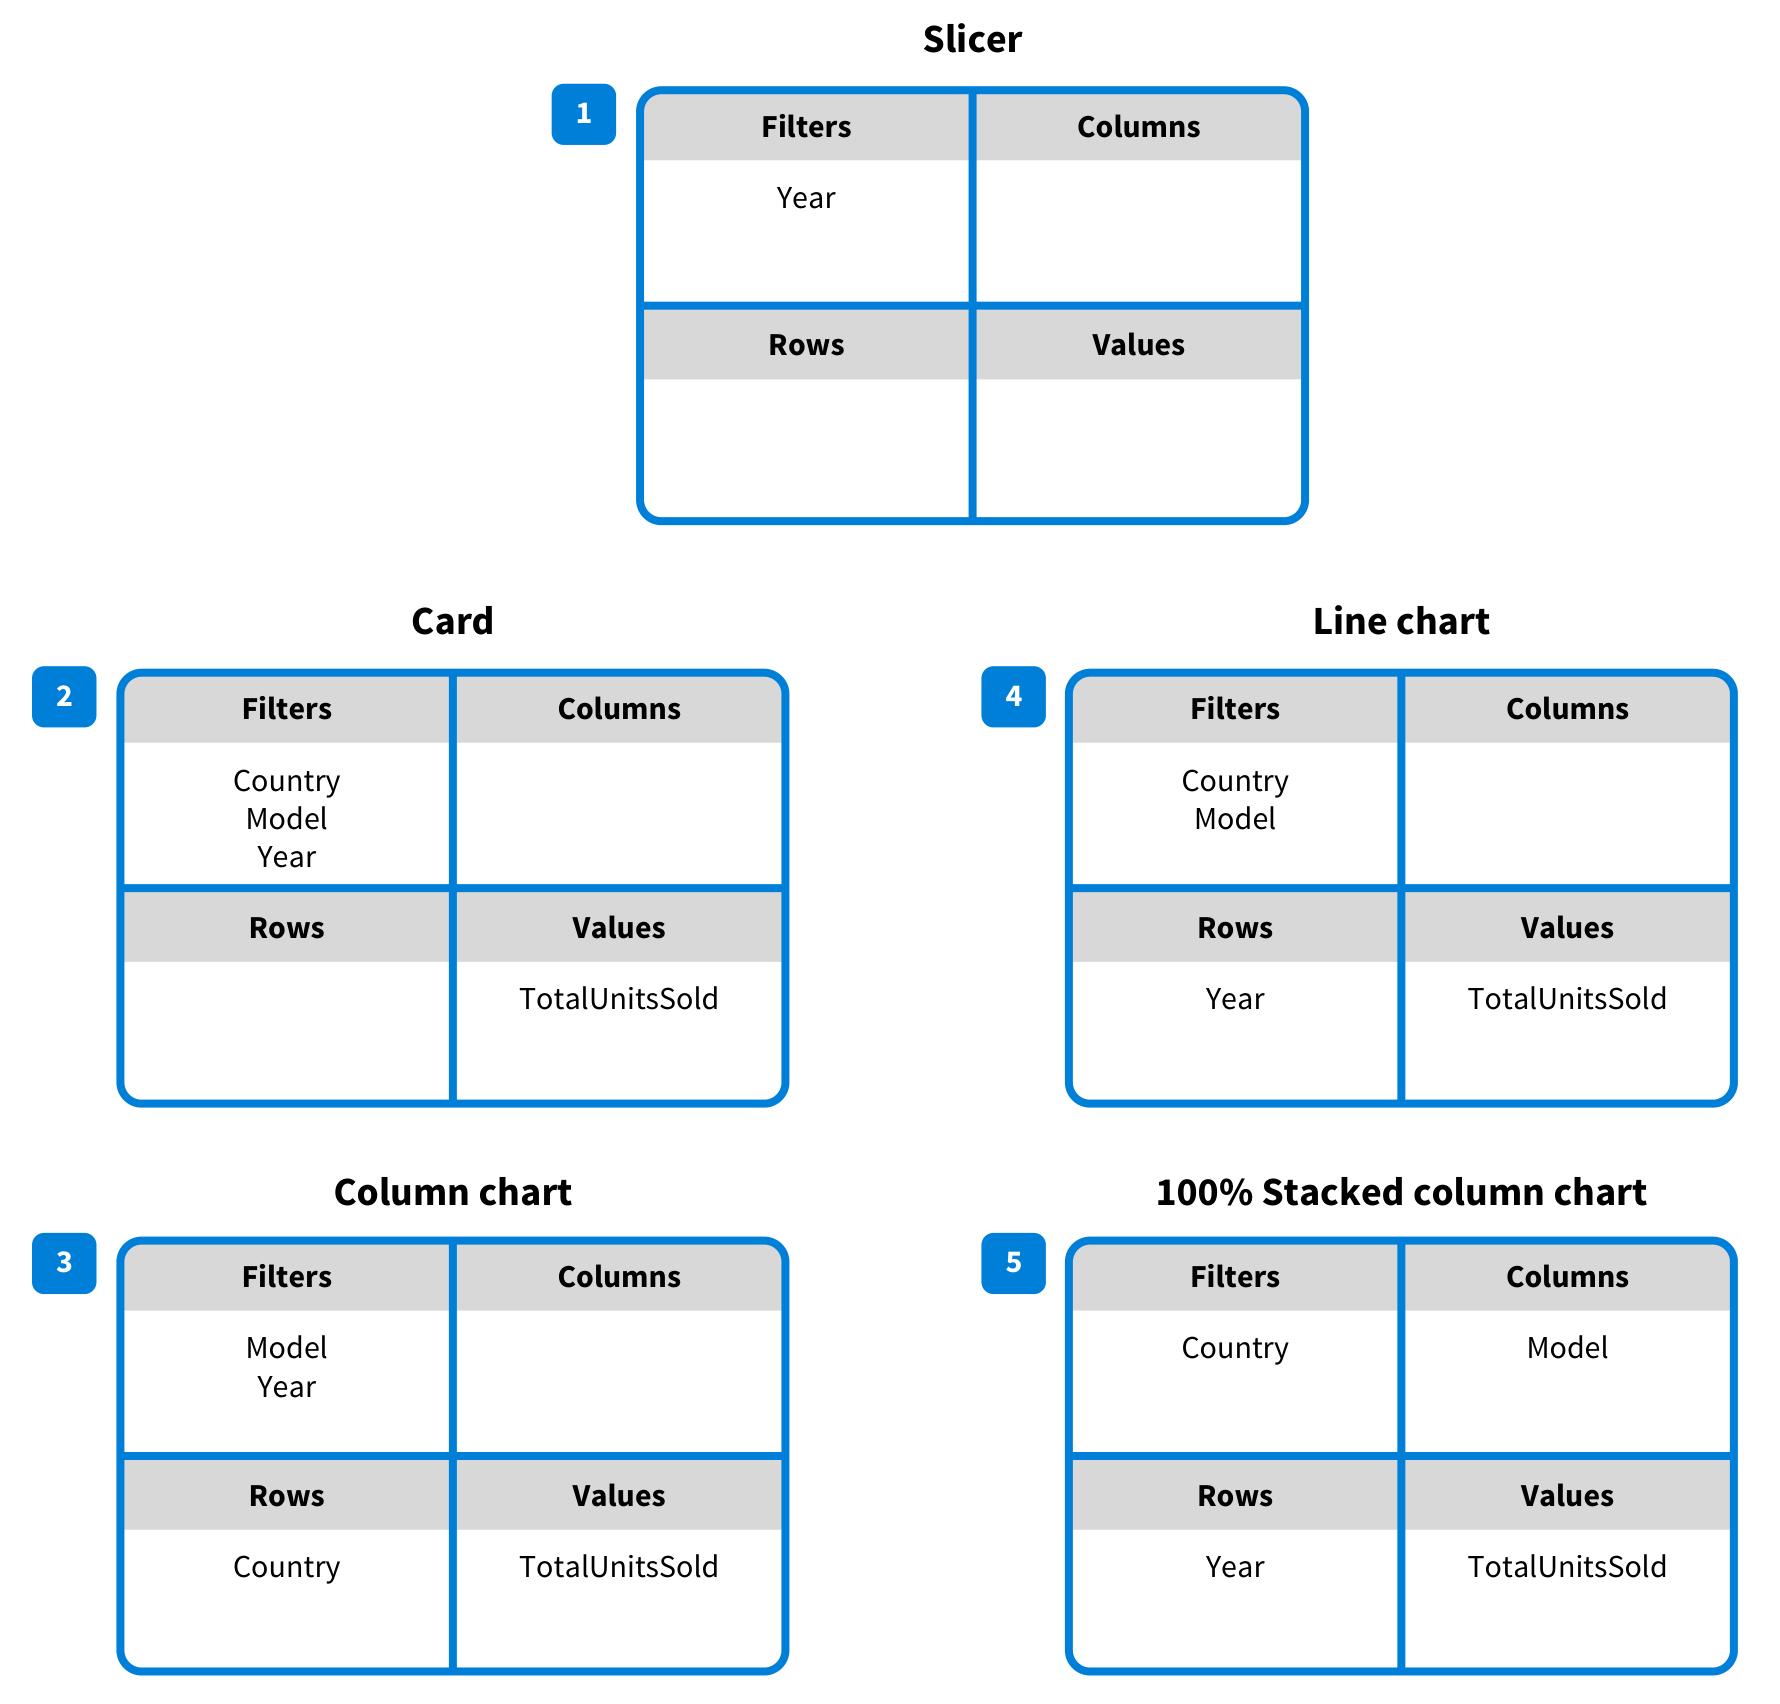
\includegraphics[width=0.95\textwidth,height=0.75\textheight,keepaspectratio]{../textbookForPractice/Figures/Ch_07/ILLUSTRATION 7.44.png}
    \end{figure}
\end{frame}

\begin{frame}{ILLUSTRATION 7.45}

    \begin{figure}[h]
        \centering
        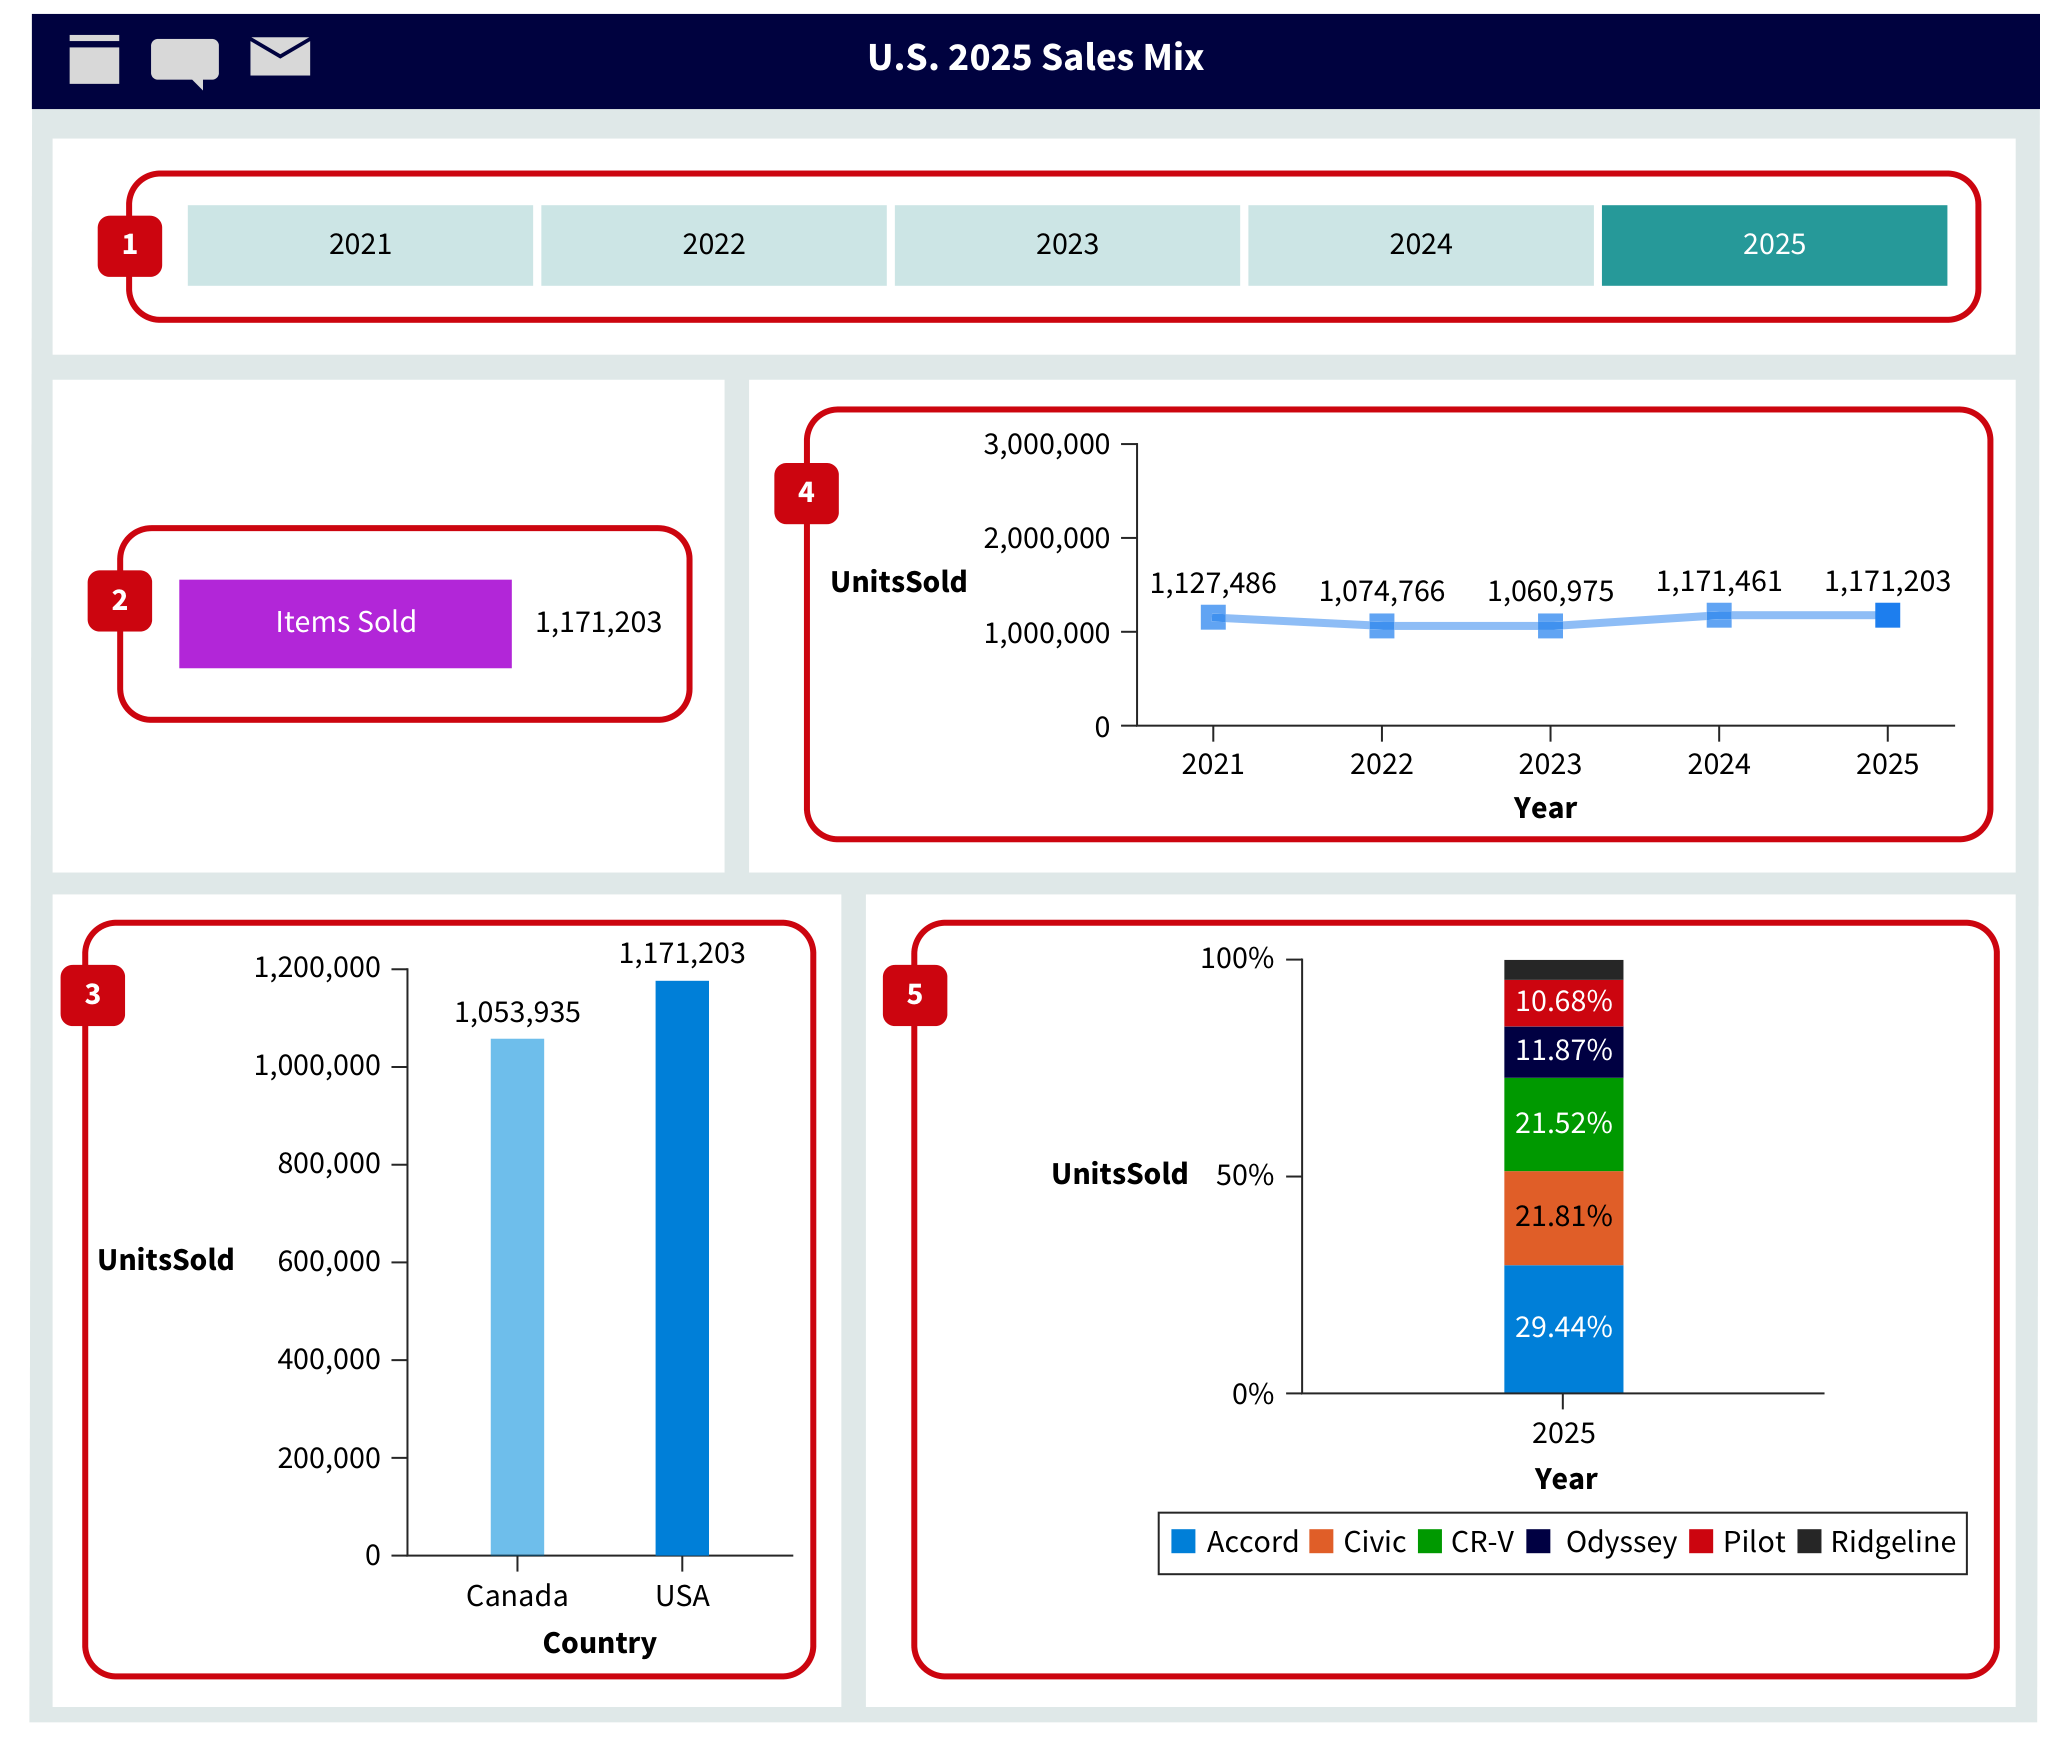
\includegraphics[width=0.95\textwidth,height=0.75\textheight,keepaspectratio]{../textbookForPractice/Figures/Ch_07/ILLUSTRATION 7.45.png}
    \end{figure}
\end{frame}

\begin{frame}{ILLUSTRATION 7.46}

    \begin{figure}[h]
        \centering
        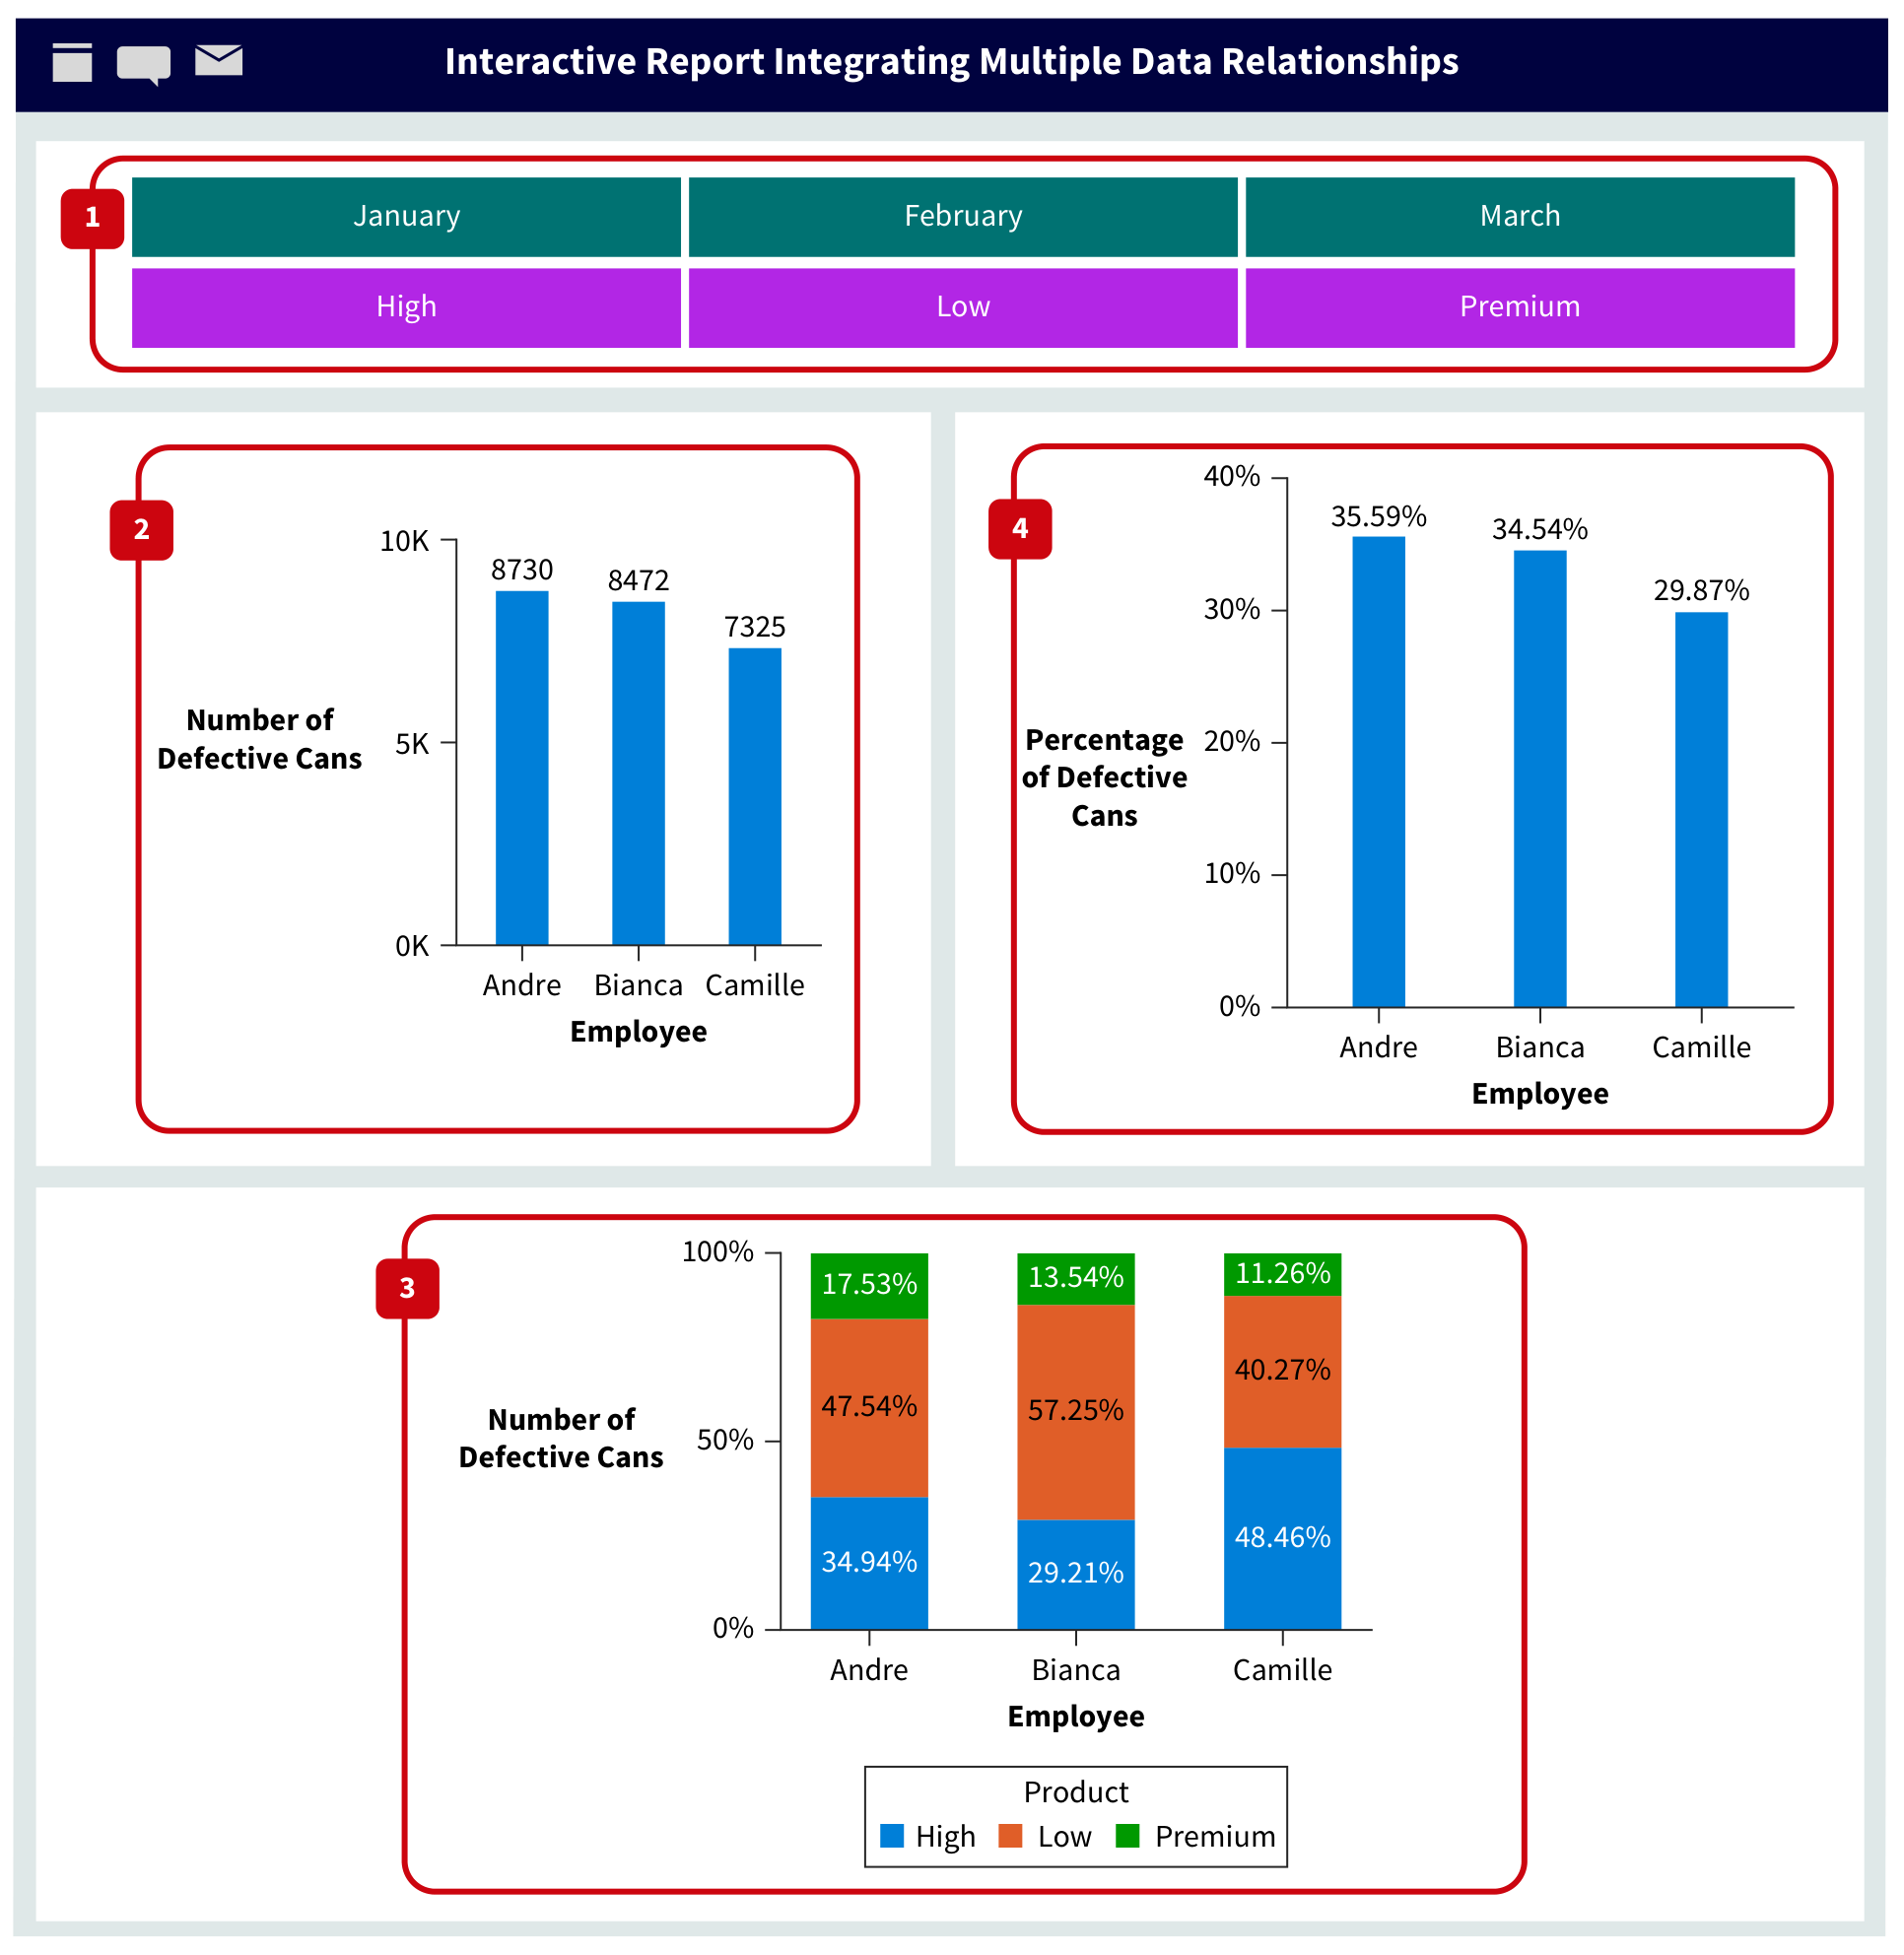
\includegraphics[width=0.95\textwidth,height=0.75\textheight,keepaspectratio]{../textbookForPractice/Figures/Ch_07/ILLUSTRATION 7.46.png}
    \end{figure}
\end{frame}

\begin{frame}{ILLUSTRATION 7.47}

    \begin{figure}[h]
        \centering
        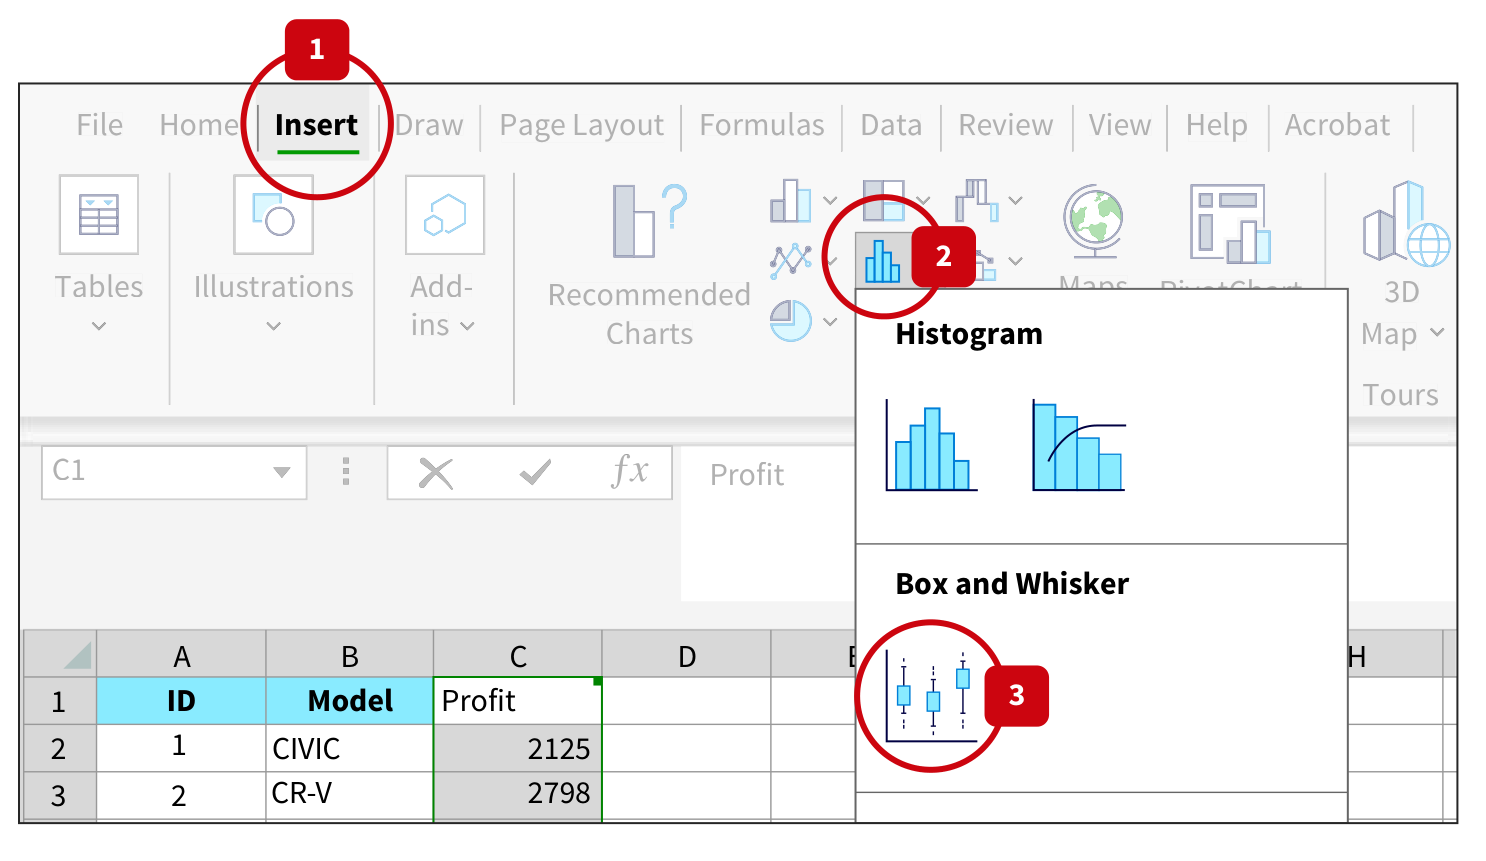
\includegraphics[width=0.95\textwidth,height=0.75\textheight,keepaspectratio]{../textbookForPractice/Figures/Ch_07/ILLUSTRATION 7.47.png}
    \end{figure}
\end{frame}

\begin{frame}{ILLUSTRATION 7.48}

    \begin{figure}[h]
        \centering
        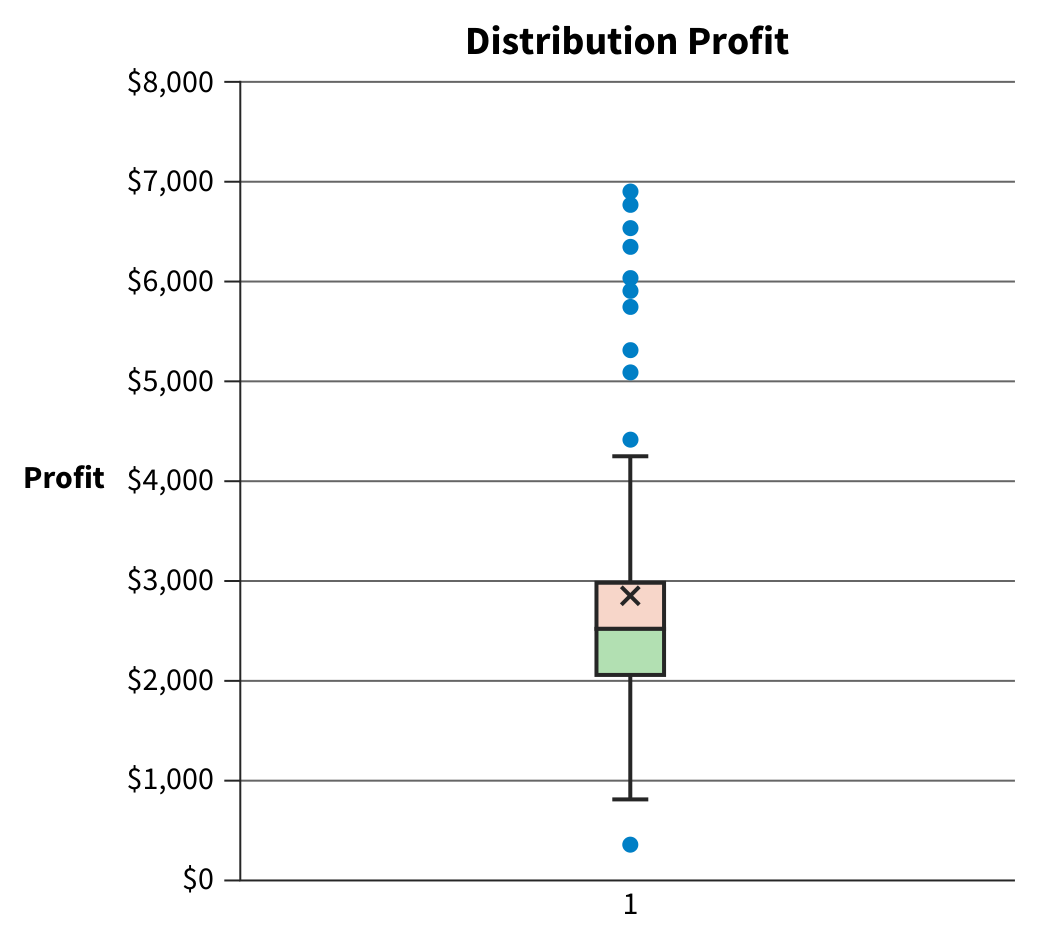
\includegraphics[width=0.95\textwidth,height=0.75\textheight,keepaspectratio]{../textbookForPractice/Figures/Ch_07/ILLUSTRATION 7.48.png}
    \end{figure}
\end{frame}

\begin{frame}{ILLUSTRATION 7.49}

    \begin{figure}[h]
        \centering
        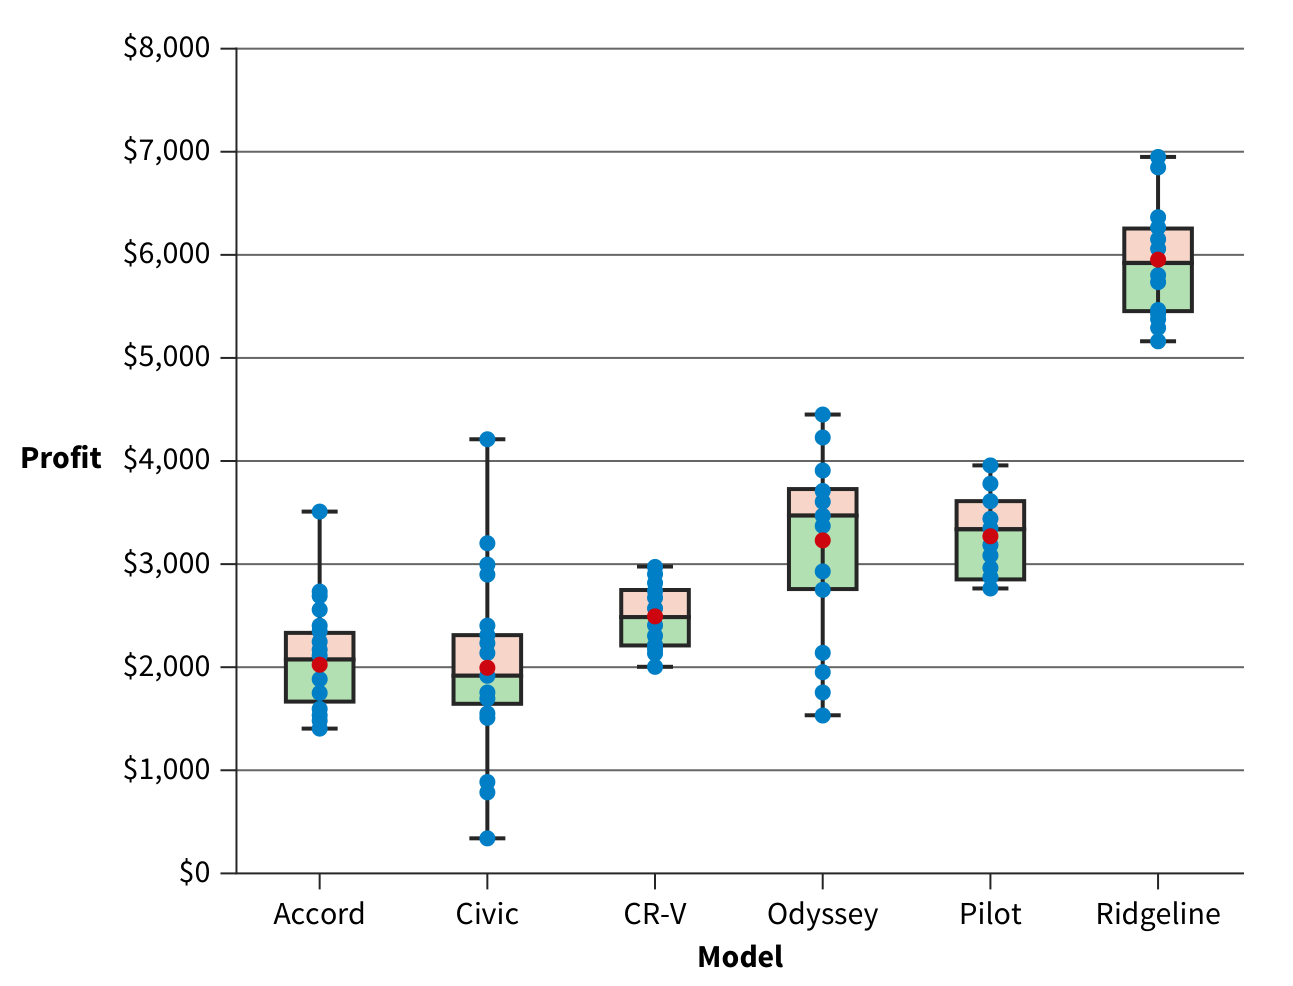
\includegraphics[width=0.95\textwidth,height=0.75\textheight,keepaspectratio]{../textbookForPractice/Figures/Ch_07/ILLUSTRATION 7.49.png}
    \end{figure}
\end{frame}

\begin{frame}{ILLUSTRATION 7.50}

    \begin{figure}[h]
        \centering
        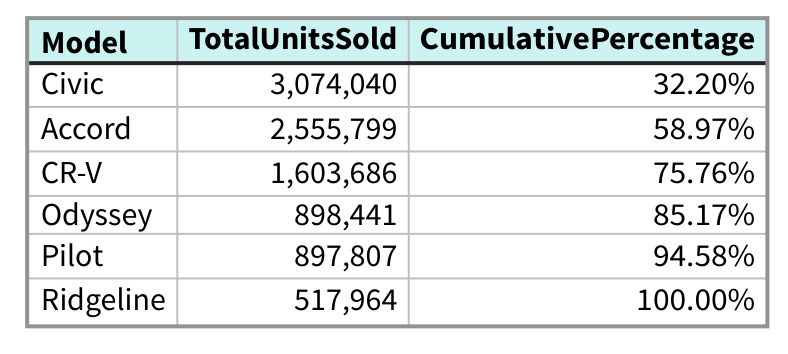
\includegraphics[width=0.95\textwidth,height=0.75\textheight,keepaspectratio]{../textbookForPractice/Figures/Ch_07/ILLUSTRATION 7.50.png}
    \end{figure}
\end{frame}

\begin{frame}{ILLUSTRATION 7.51}

    \begin{figure}[h]
        \centering
        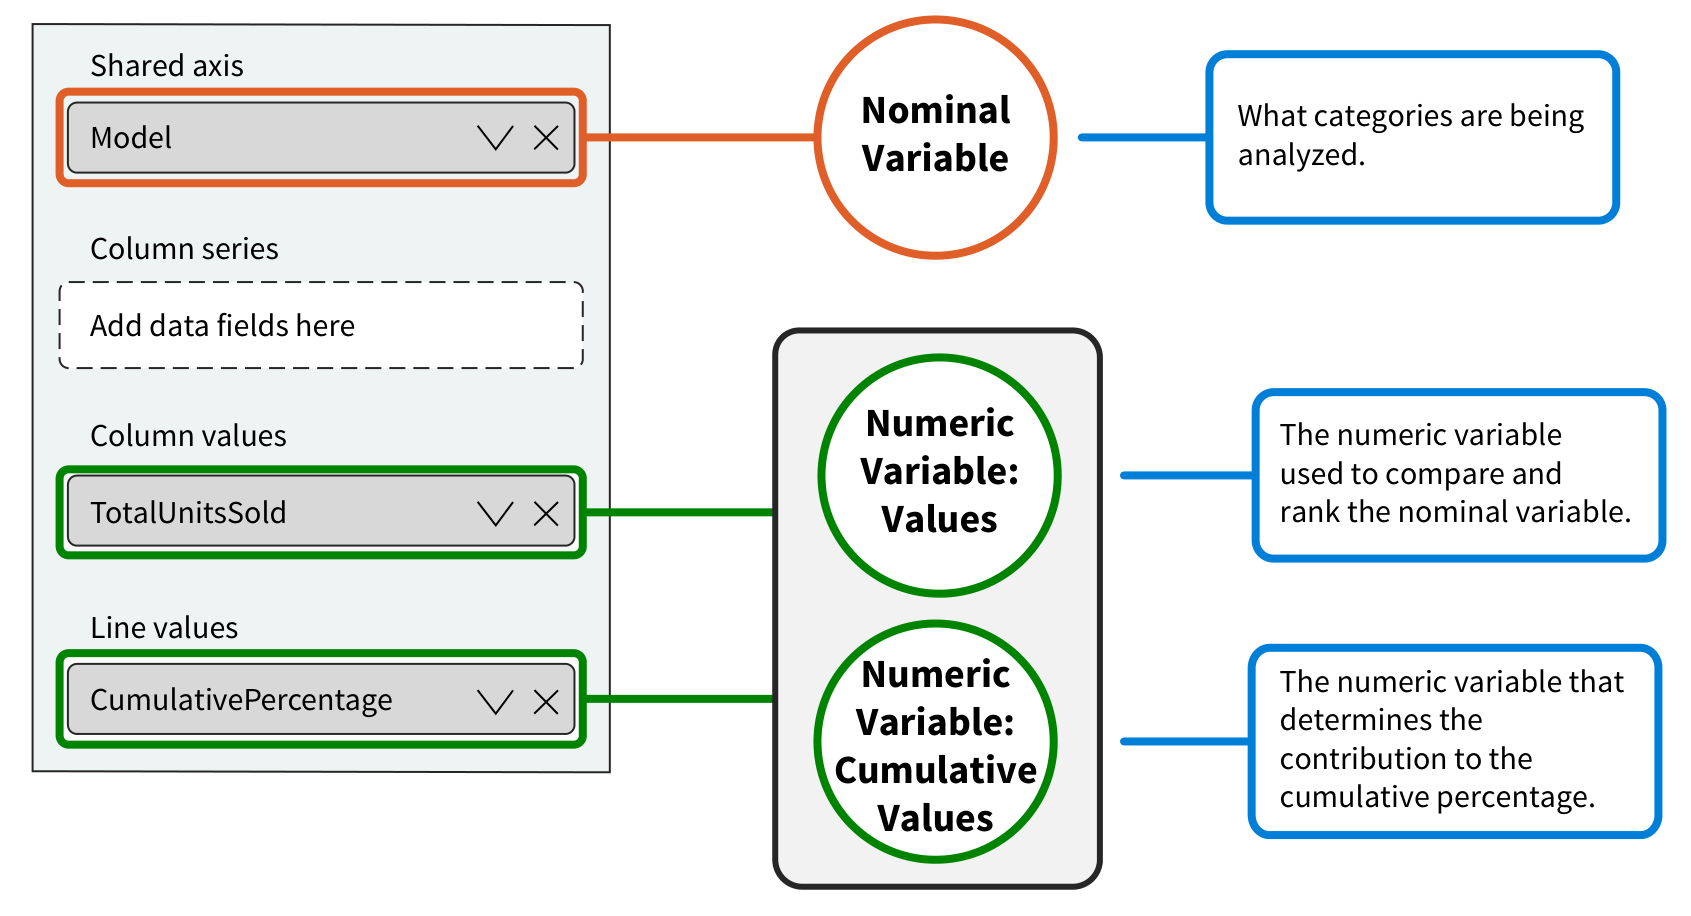
\includegraphics[width=0.95\textwidth,height=0.75\textheight,keepaspectratio]{../textbookForPractice/Figures/Ch_07/ILLUSTRATION 7.51.png}
    \end{figure}
\end{frame}

\begin{frame}{ILLUSTRATION 7.52}

    \begin{figure}[h]
        \centering
        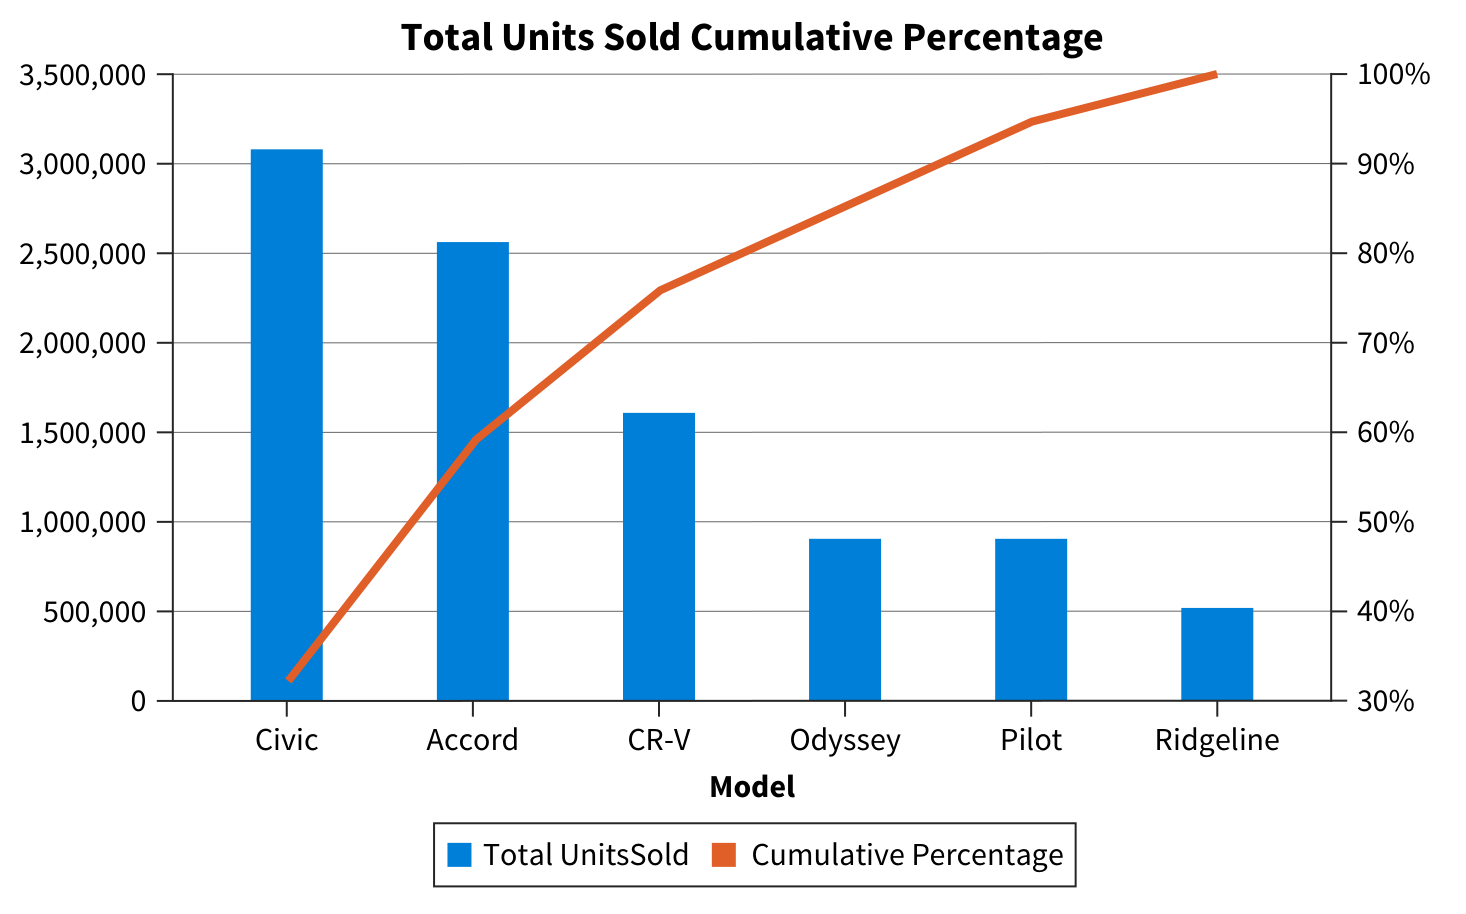
\includegraphics[width=0.95\textwidth,height=0.75\textheight,keepaspectratio]{../textbookForPractice/Figures/Ch_07/ILLUSTRATION 7.52.png}
    \end{figure}
\end{frame}

\begin{frame}{Bài tập Ngắn (Brief Exercises)}
\begin{center}
    \Huge \textbf{Phần Bài tập Ngắn} \\
    \vspace{0.5cm}
    \Large Brief Exercises (BE)
\end{center}
\end{frame}

\begin{frame}{BE 7.6 \& BE 7.7}
    \begin{columns}
        \begin{column}{0.5\textwidth}
            \begin{figure}[h]
                \centering
                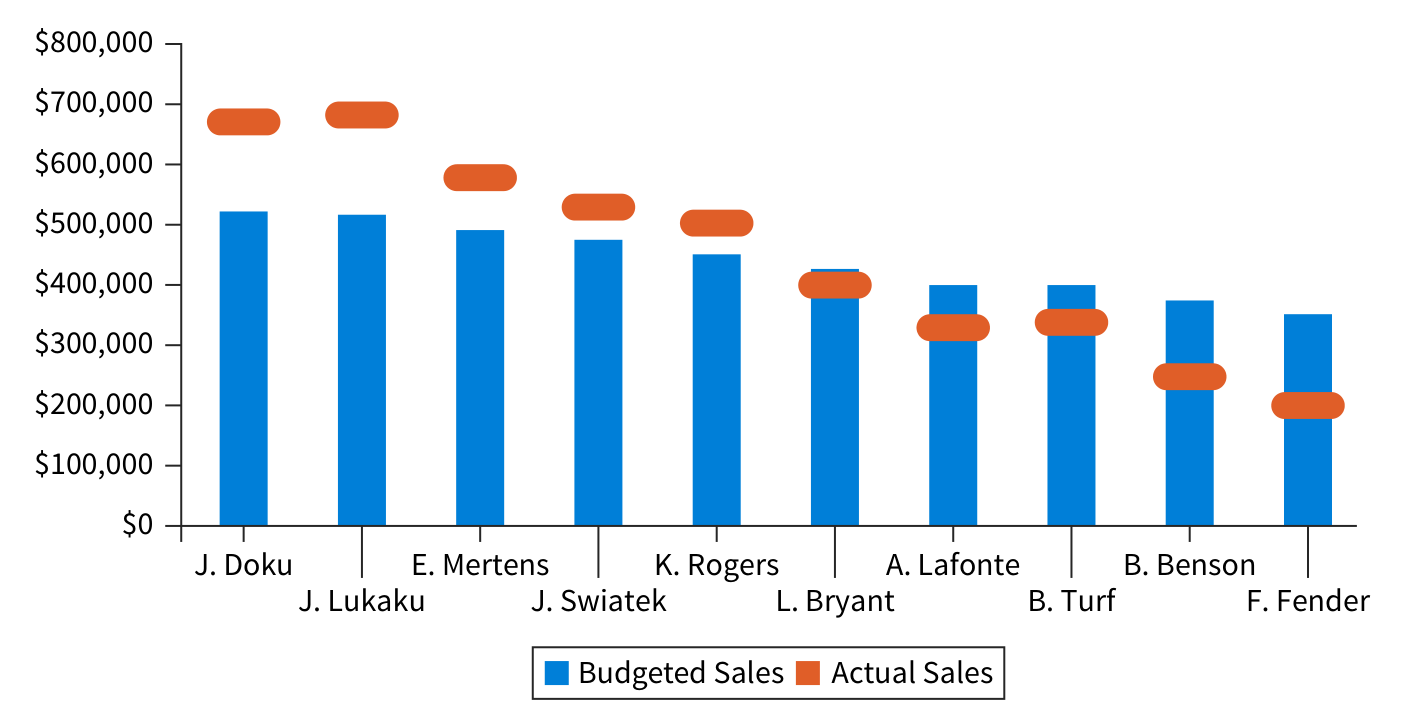
\includegraphics[width=\textwidth,height=0.7\textheight,keepaspectratio]{../textbookForPractice/Figures/Ch_07/BE 7.6.png}
            \end{figure}
        \end{column}
        \begin{column}{0.5\textwidth}
            \begin{figure}[h]
                \centering
                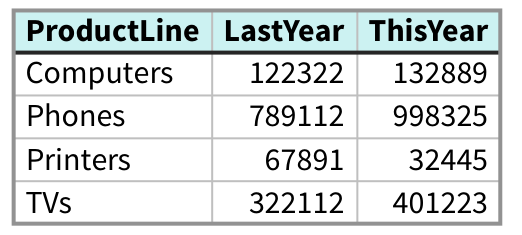
\includegraphics[width=\textwidth,height=0.7\textheight,keepaspectratio]{../textbookForPractice/Figures/Ch_07/BE 7.7.png}
            \end{figure}
        \end{column}
    \end{columns}
\end{frame}

\begin{frame}{BE 7.8 \& BE 7.9}
    \begin{columns}
        \begin{column}{0.5\textwidth}
            \begin{figure}[h]
                \centering
                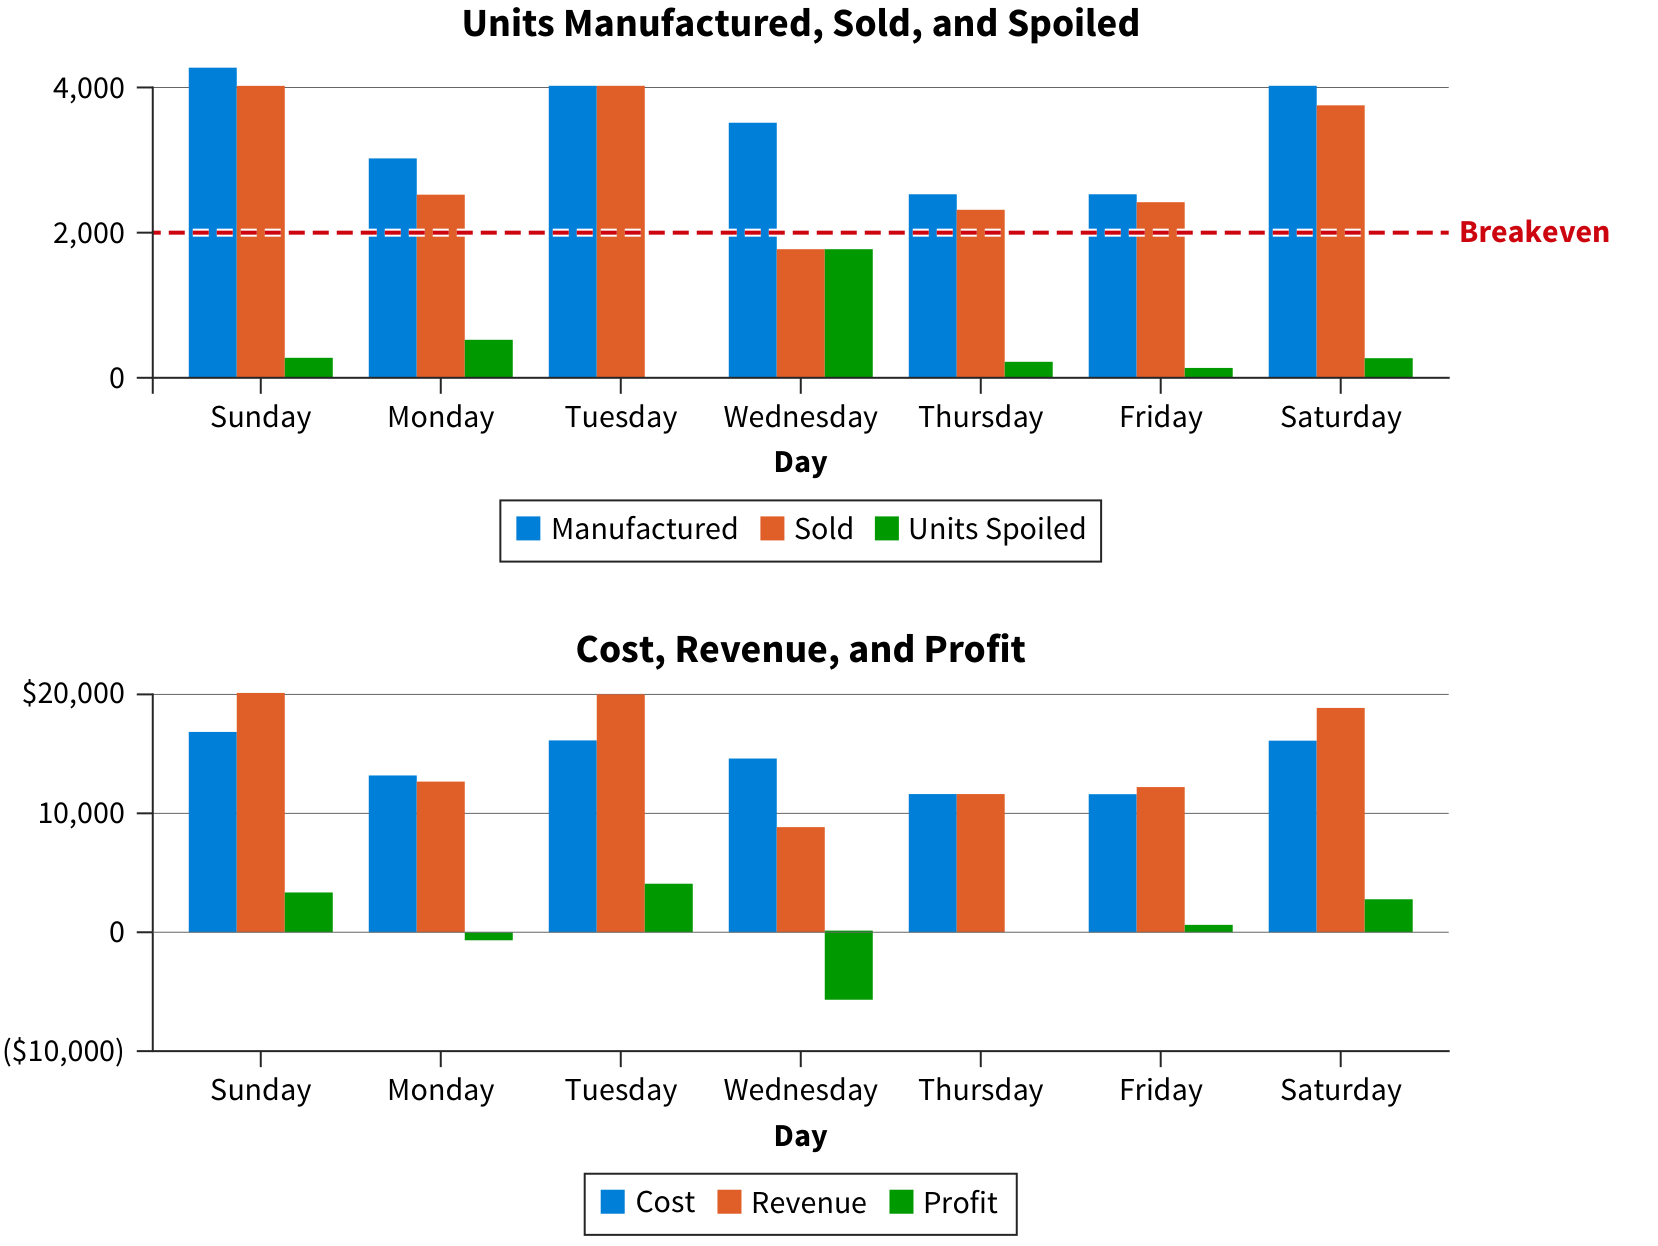
\includegraphics[width=\textwidth,height=0.7\textheight,keepaspectratio]{../textbookForPractice/Figures/Ch_07/BE 7.8.png}
            \end{figure}
        \end{column}
        \begin{column}{0.5\textwidth}
            \begin{figure}[h]
                \centering
                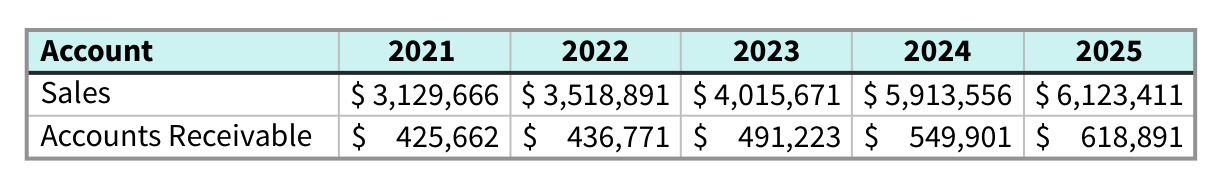
\includegraphics[width=\textwidth,height=0.7\textheight,keepaspectratio]{../textbookForPractice/Figures/Ch_07/BE 7.9.png}
            \end{figure}
        \end{column}
    \end{columns}
\end{frame}

\begin{frame}{BE 7.10 \& BE 7.11A}
    \begin{columns}
        \begin{column}{0.5\textwidth}
            \begin{figure}[h]
                \centering
                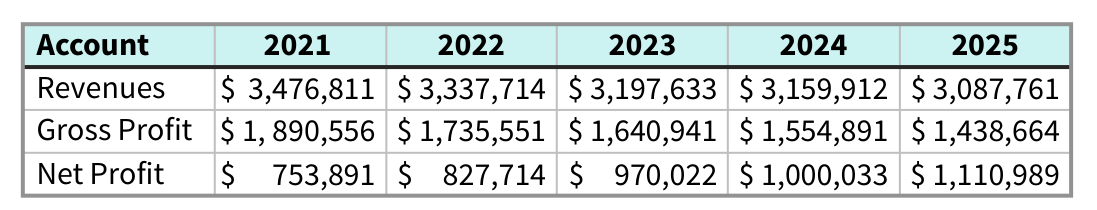
\includegraphics[width=\textwidth,height=0.7\textheight,keepaspectratio]{../textbookForPractice/Figures/Ch_07/BE 7.10.png}
            \end{figure}
        \end{column}
        \begin{column}{0.5\textwidth}
            \begin{figure}[h]
                \centering
                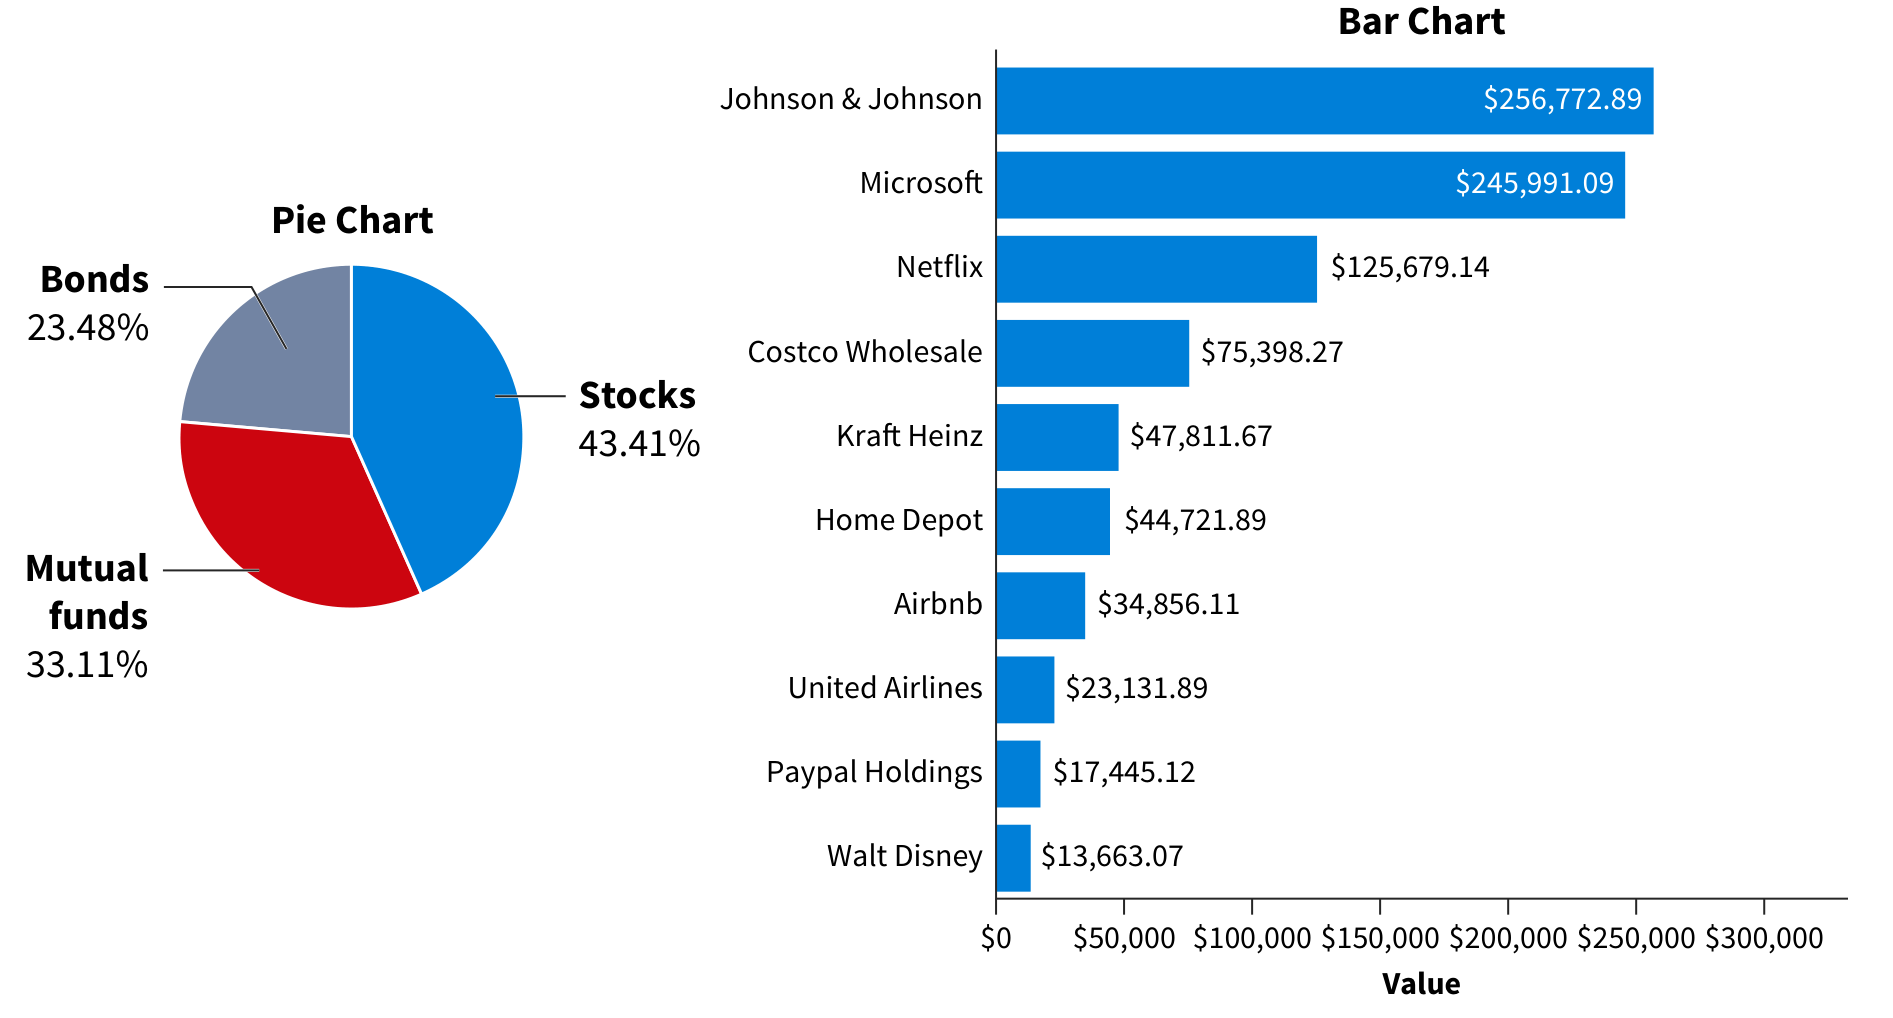
\includegraphics[width=\textwidth,height=0.7\textheight,keepaspectratio]{../textbookForPractice/Figures/Ch_07/BE 7.11A.png}
            \end{figure}
        \end{column}
    \end{columns}
\end{frame}

\begin{frame}{BE 7.11B \& BE 7.12A}
    \begin{columns}
        \begin{column}{0.5\textwidth}
            \begin{figure}[h]
                \centering
                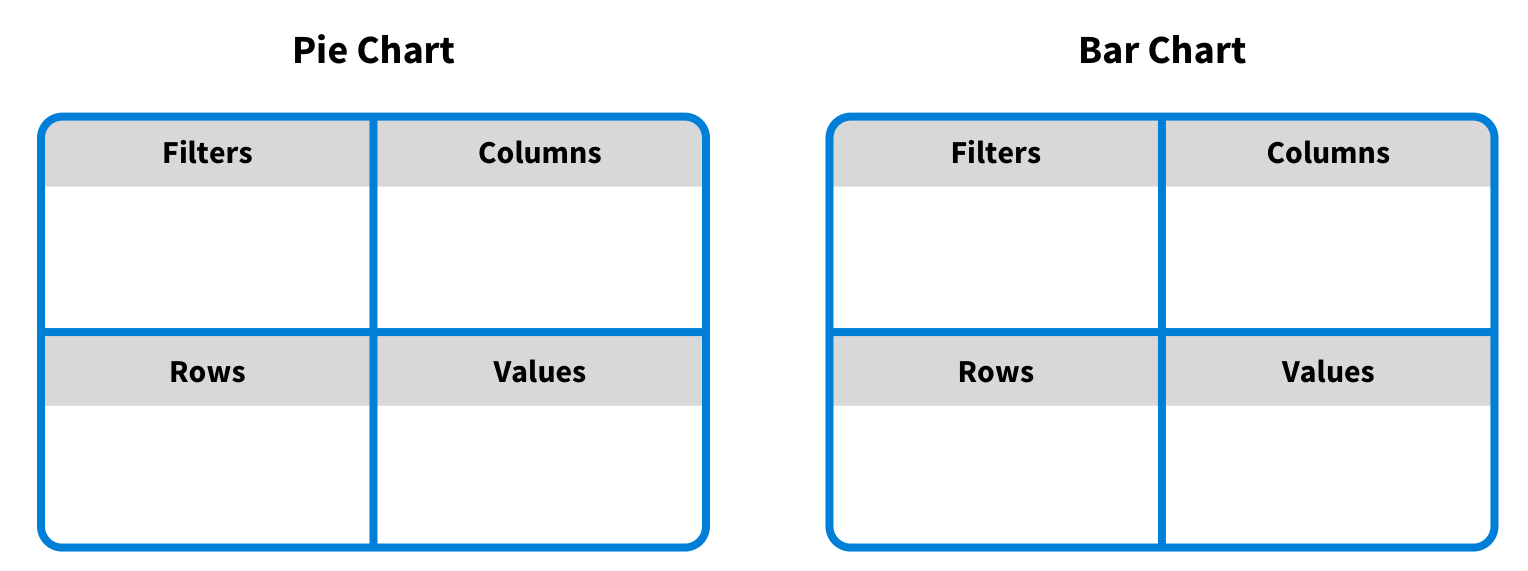
\includegraphics[width=\textwidth,height=0.7\textheight,keepaspectratio]{../textbookForPractice/Figures/Ch_07/BE 7.11B.png}
            \end{figure}
        \end{column}
        \begin{column}{0.5\textwidth}
            \begin{figure}[h]
                \centering
                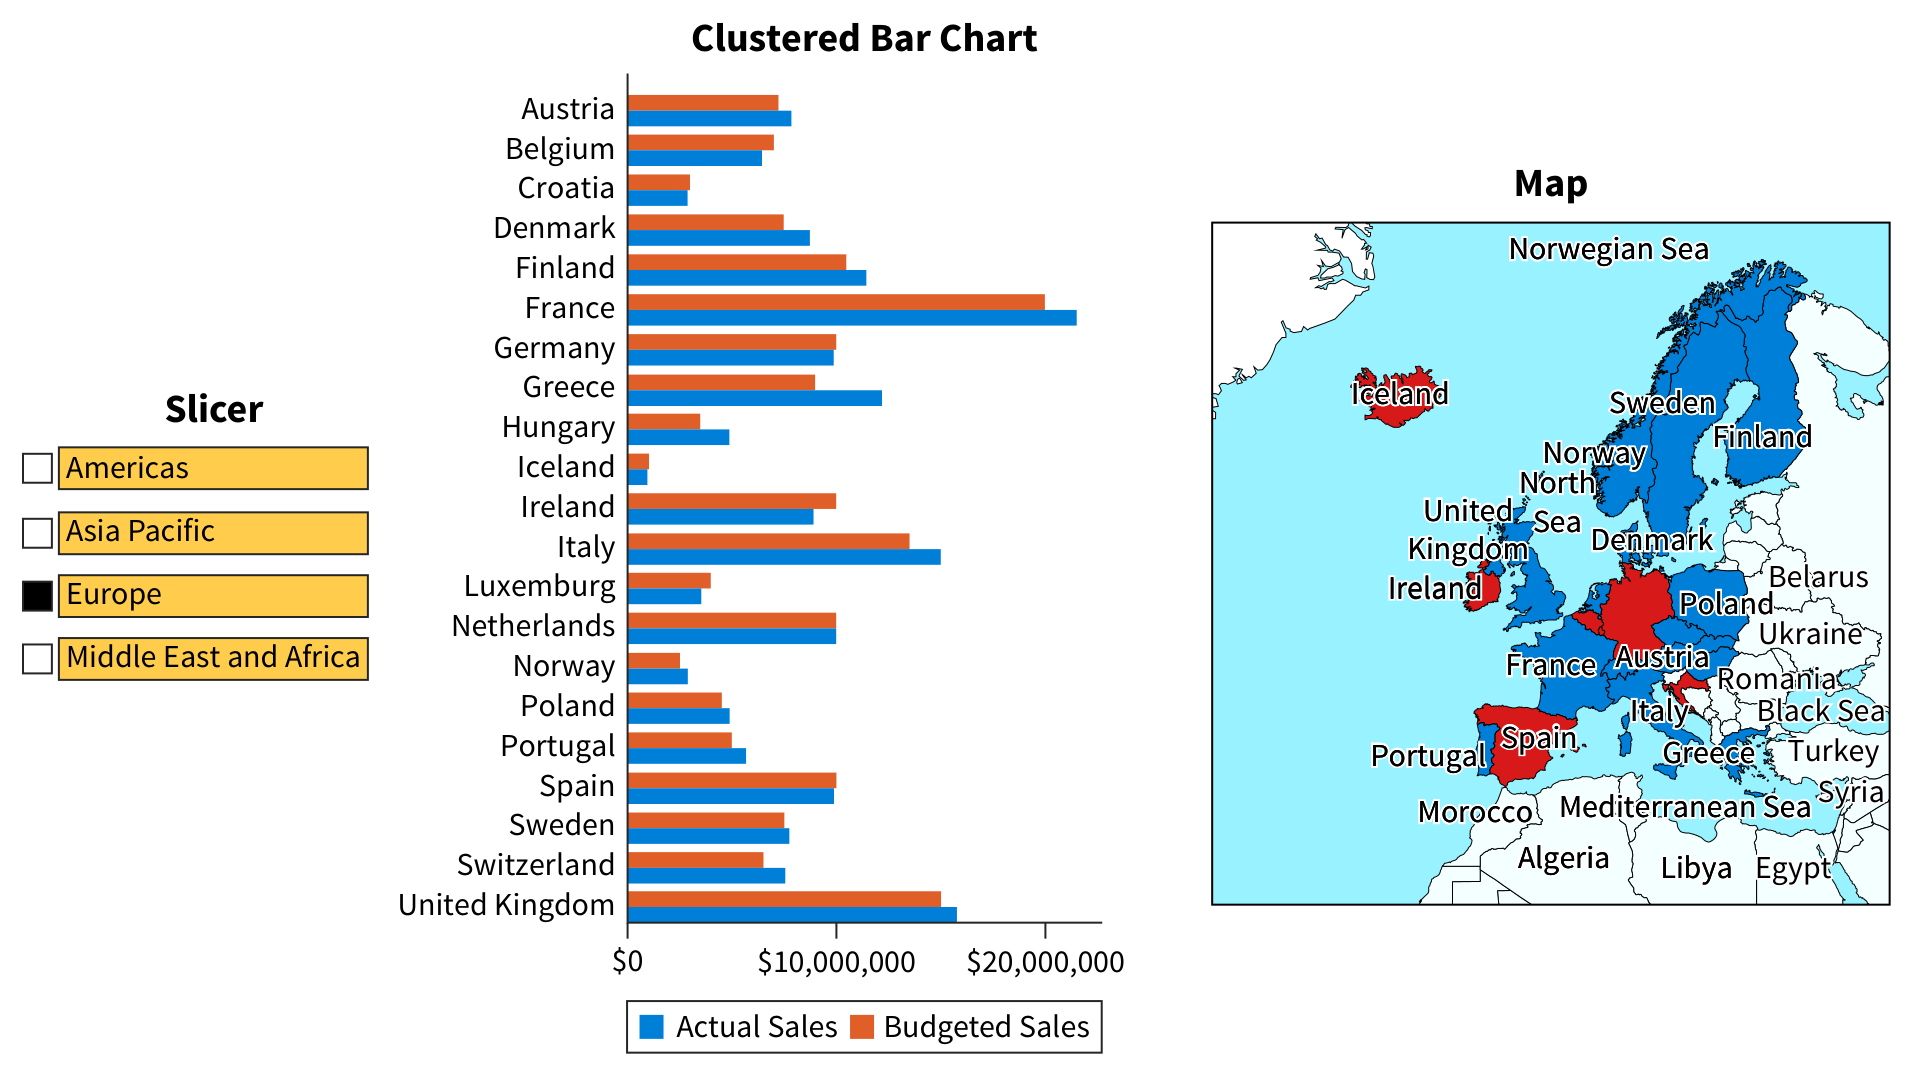
\includegraphics[width=\textwidth,height=0.7\textheight,keepaspectratio]{../textbookForPractice/Figures/Ch_07/BE 7.12A.png}
            \end{figure}
        \end{column}
    \end{columns}
\end{frame}

\begin{frame}{BE 7.12B}

    \begin{figure}[h]
        \centering
        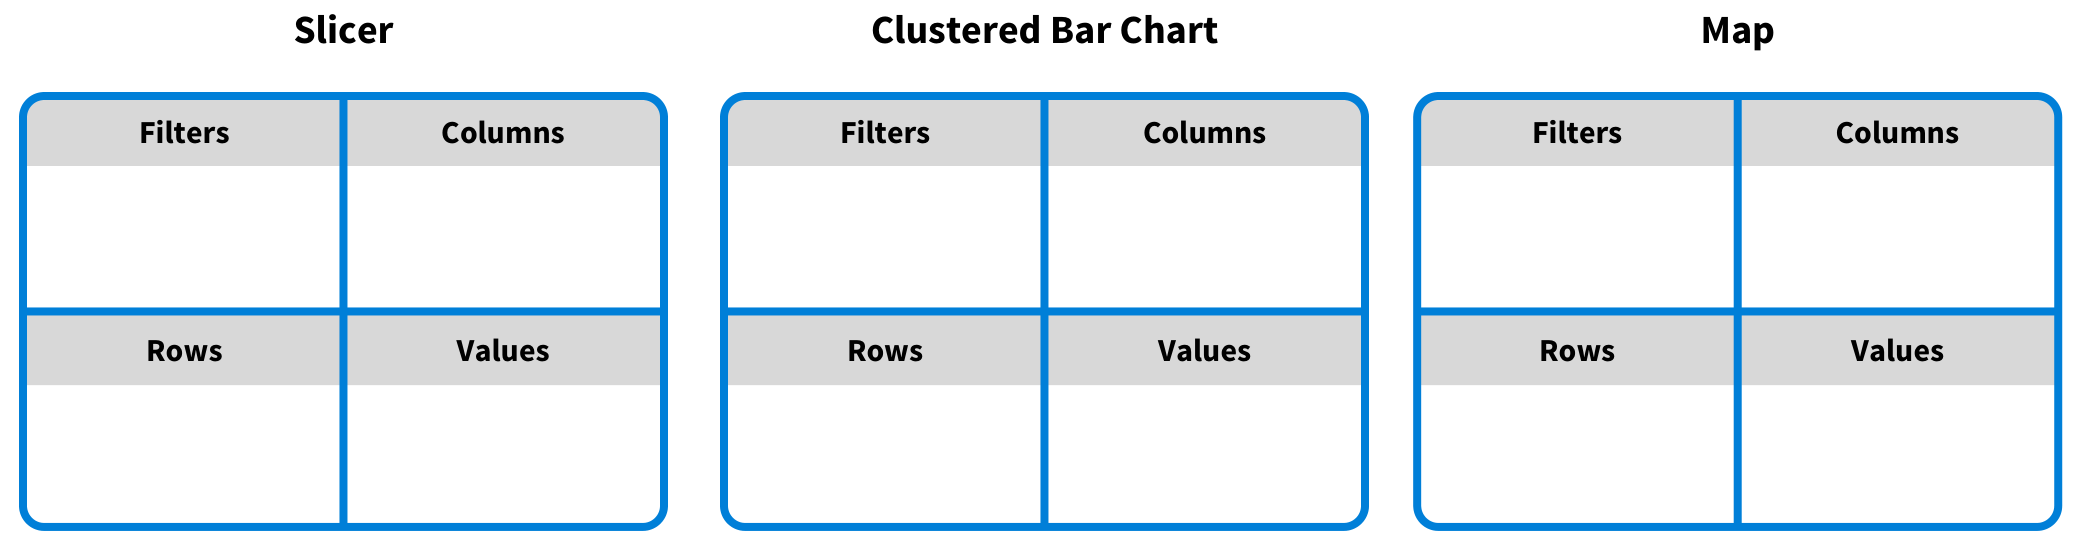
\includegraphics[width=0.95\textwidth,height=0.75\textheight,keepaspectratio]{../textbookForPractice/Figures/Ch_07/BE 7.12B.png}
    \end{figure}
\end{frame}

\begin{frame}{Bài tập (Exercises)}
\begin{center}
    \Huge \textbf{Phần Bài tập} \\
    \vspace{0.5cm}
    \Large Exercises (EX)
\end{center}
\end{frame}

\begin{frame}{EX 7.3 \& EX 7.4}
    \begin{columns}
        \begin{column}{0.5\textwidth}
            \begin{figure}[h]
                \centering
                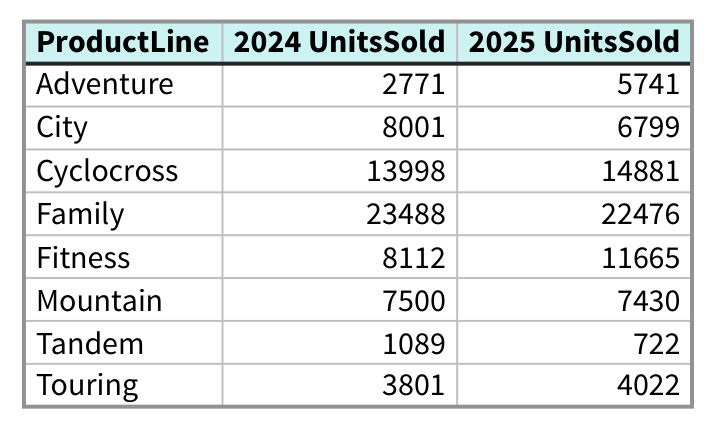
\includegraphics[width=\textwidth,height=0.7\textheight,keepaspectratio]{../textbookForPractice/Figures/Ch_07/EX 7.3.png}
            \end{figure}
        \end{column}
        \begin{column}{0.5\textwidth}
            \begin{figure}[h]
                \centering
                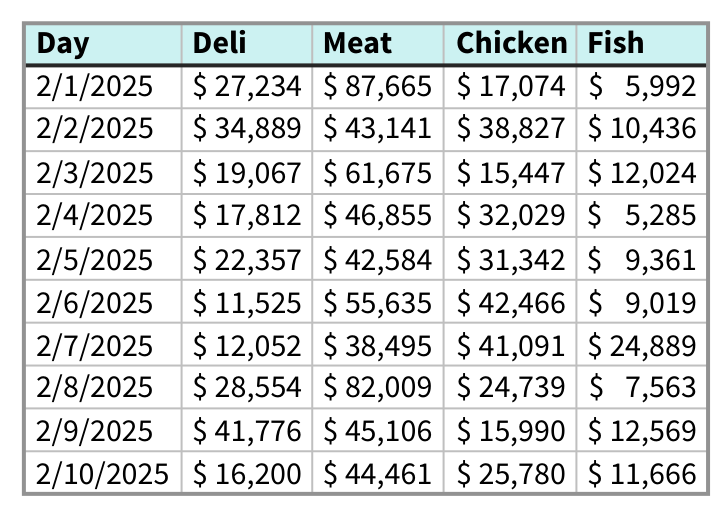
\includegraphics[width=\textwidth,height=0.7\textheight,keepaspectratio]{../textbookForPractice/Figures/Ch_07/EX 7.4.png}
            \end{figure}
        \end{column}
    \end{columns}
\end{frame}

\begin{frame}{EX 7.5 \& EX 7.6}
    \begin{columns}
        \begin{column}{0.5\textwidth}
            \begin{figure}[h]
                \centering
                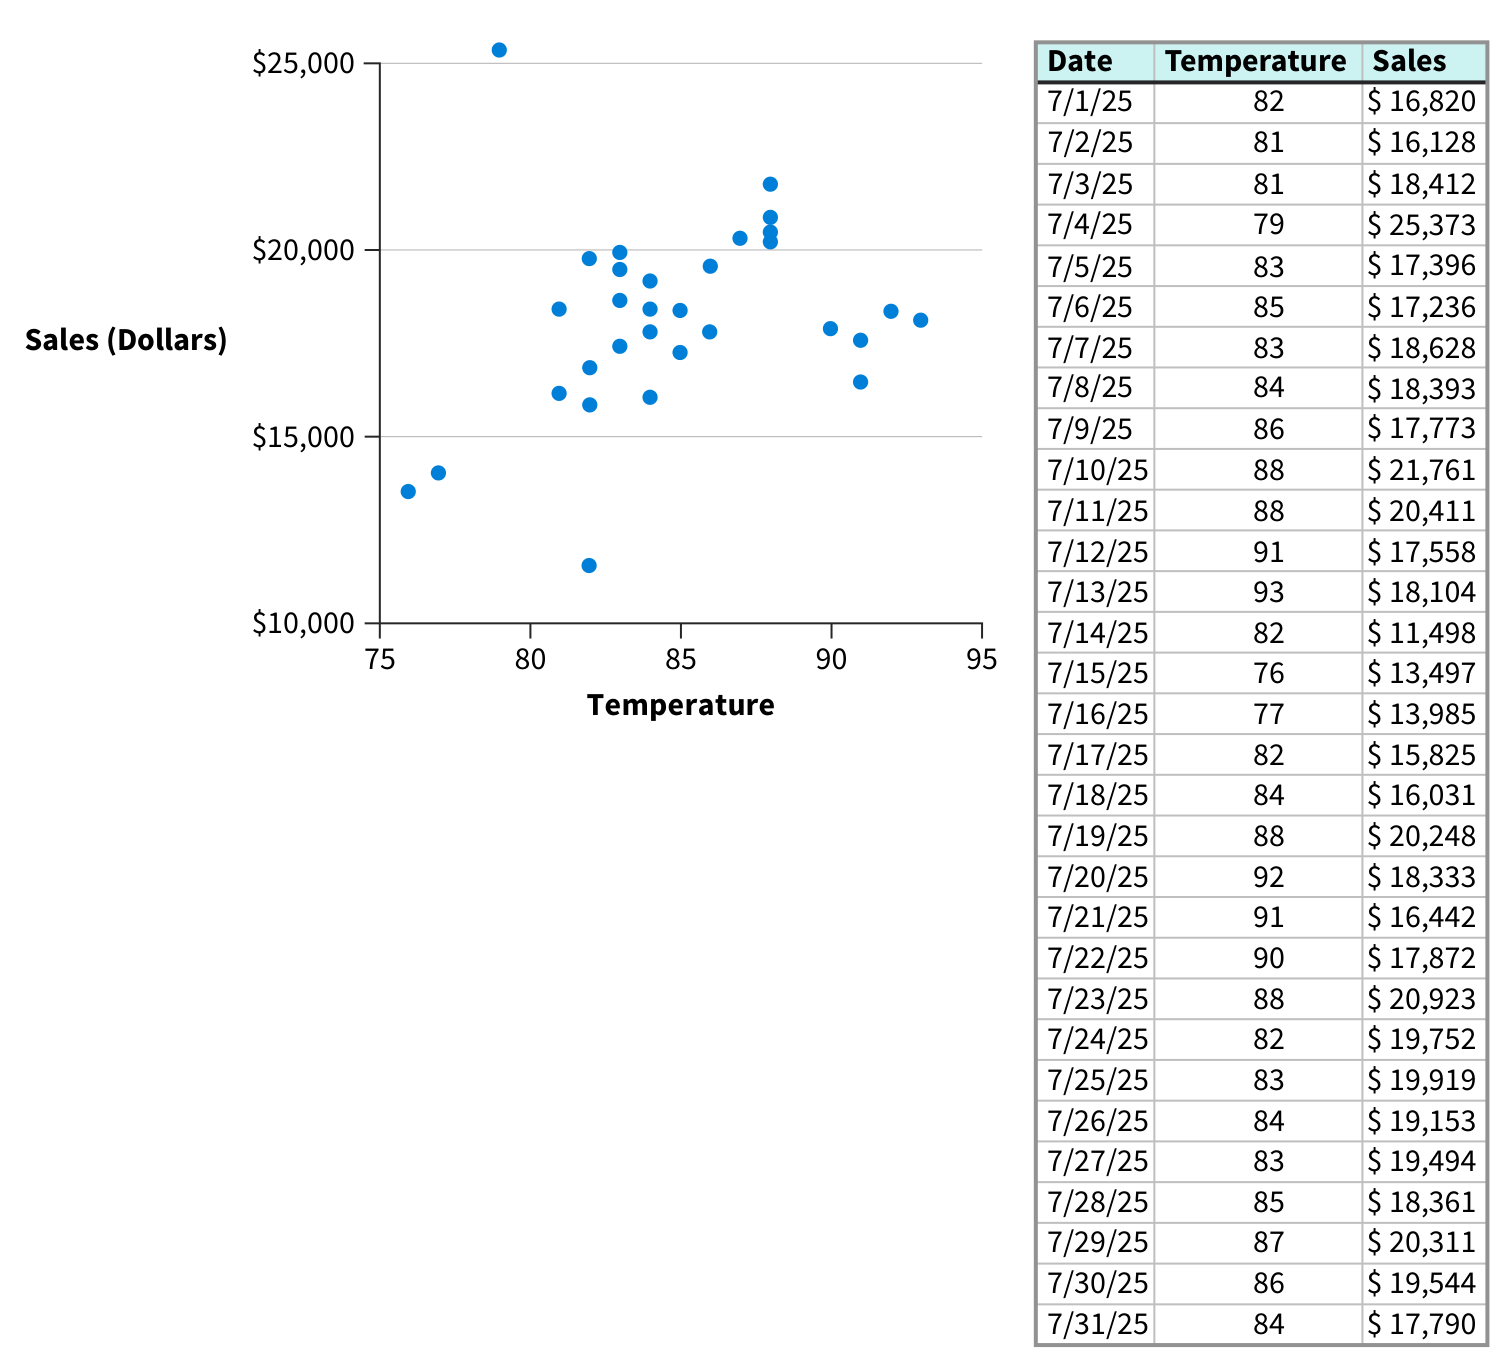
\includegraphics[width=\textwidth,height=0.7\textheight,keepaspectratio]{../textbookForPractice/Figures/Ch_07/EX 7.5.png}
            \end{figure}
        \end{column}
        \begin{column}{0.5\textwidth}
            \begin{figure}[h]
                \centering
                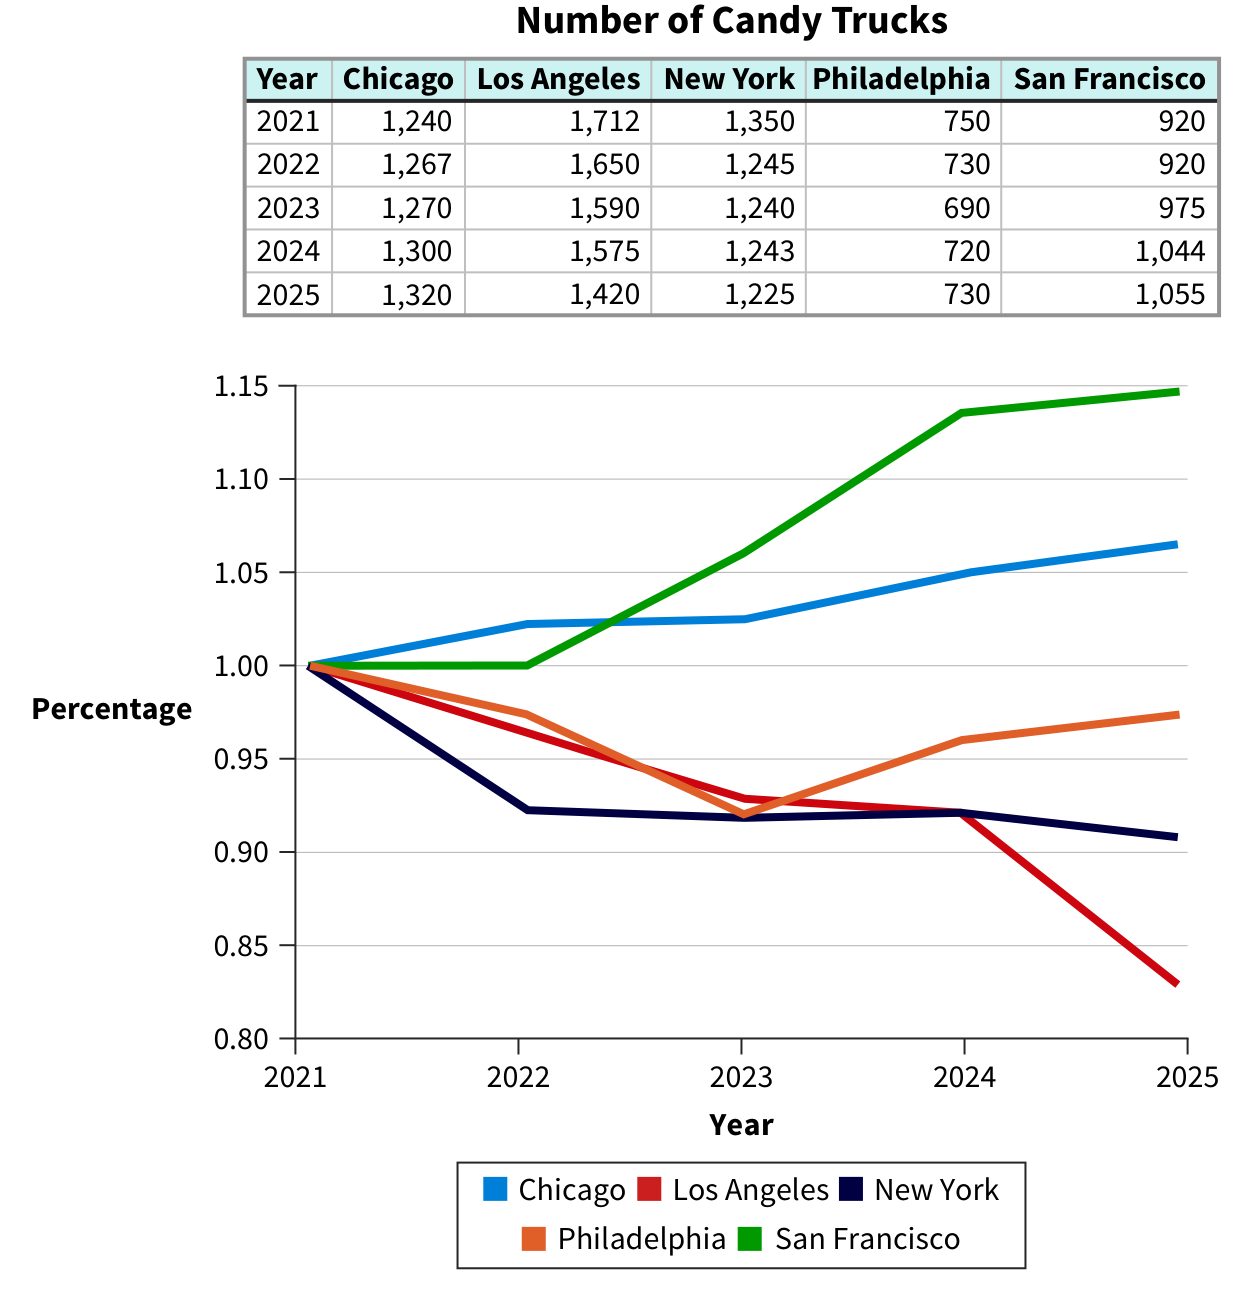
\includegraphics[width=\textwidth,height=0.7\textheight,keepaspectratio]{../textbookForPractice/Figures/Ch_07/EX 7.6.png}
            \end{figure}
        \end{column}
    \end{columns}
\end{frame}

\begin{frame}{EX 7.7 \& EX 7.8}
    \begin{columns}
        \begin{column}{0.5\textwidth}
            \begin{figure}[h]
                \centering
                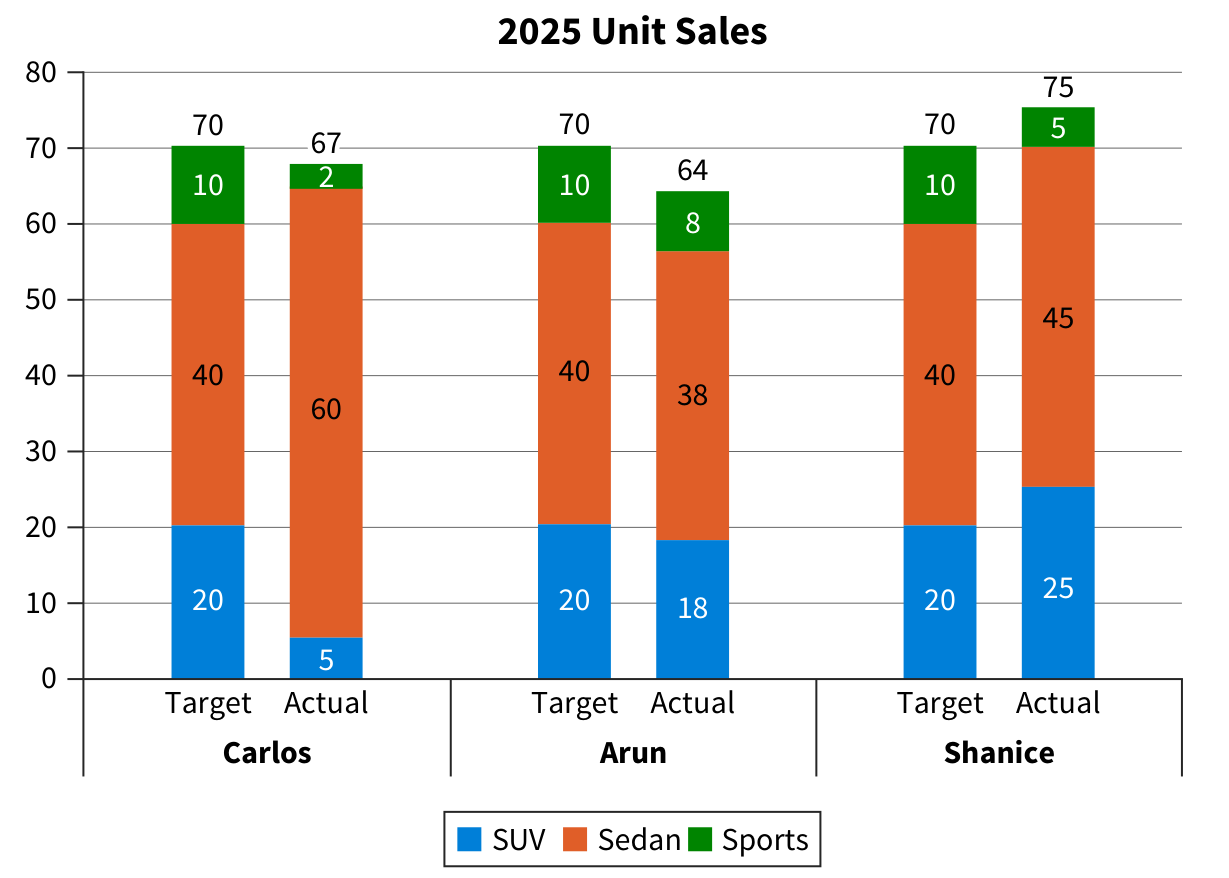
\includegraphics[width=\textwidth,height=0.7\textheight,keepaspectratio]{../textbookForPractice/Figures/Ch_07/EX 7.7.png}
            \end{figure}
        \end{column}
        \begin{column}{0.5\textwidth}
            \begin{figure}[h]
                \centering
                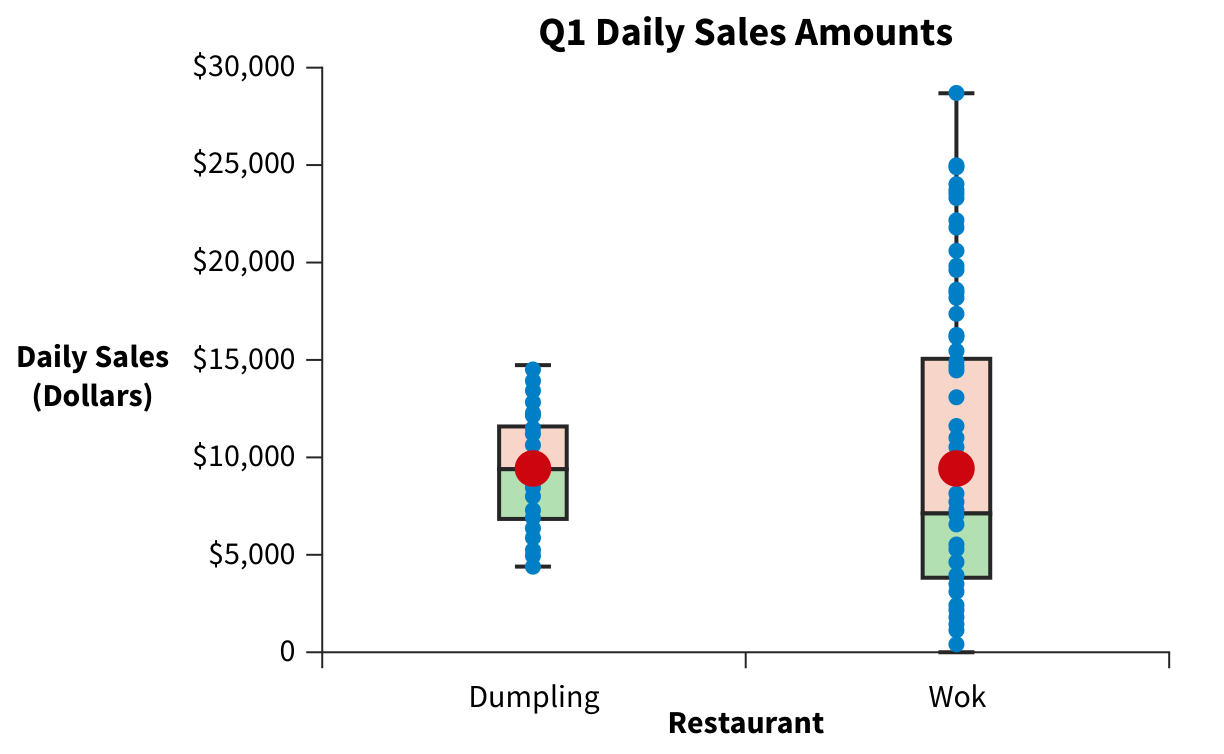
\includegraphics[width=\textwidth,height=0.7\textheight,keepaspectratio]{../textbookForPractice/Figures/Ch_07/EX 7.8.png}
            \end{figure}
        \end{column}
    \end{columns}
\end{frame}

\begin{frame}{EX 7.9 \& EX 7.10A}
    \begin{columns}
        \begin{column}{0.5\textwidth}
            \begin{figure}[h]
                \centering
                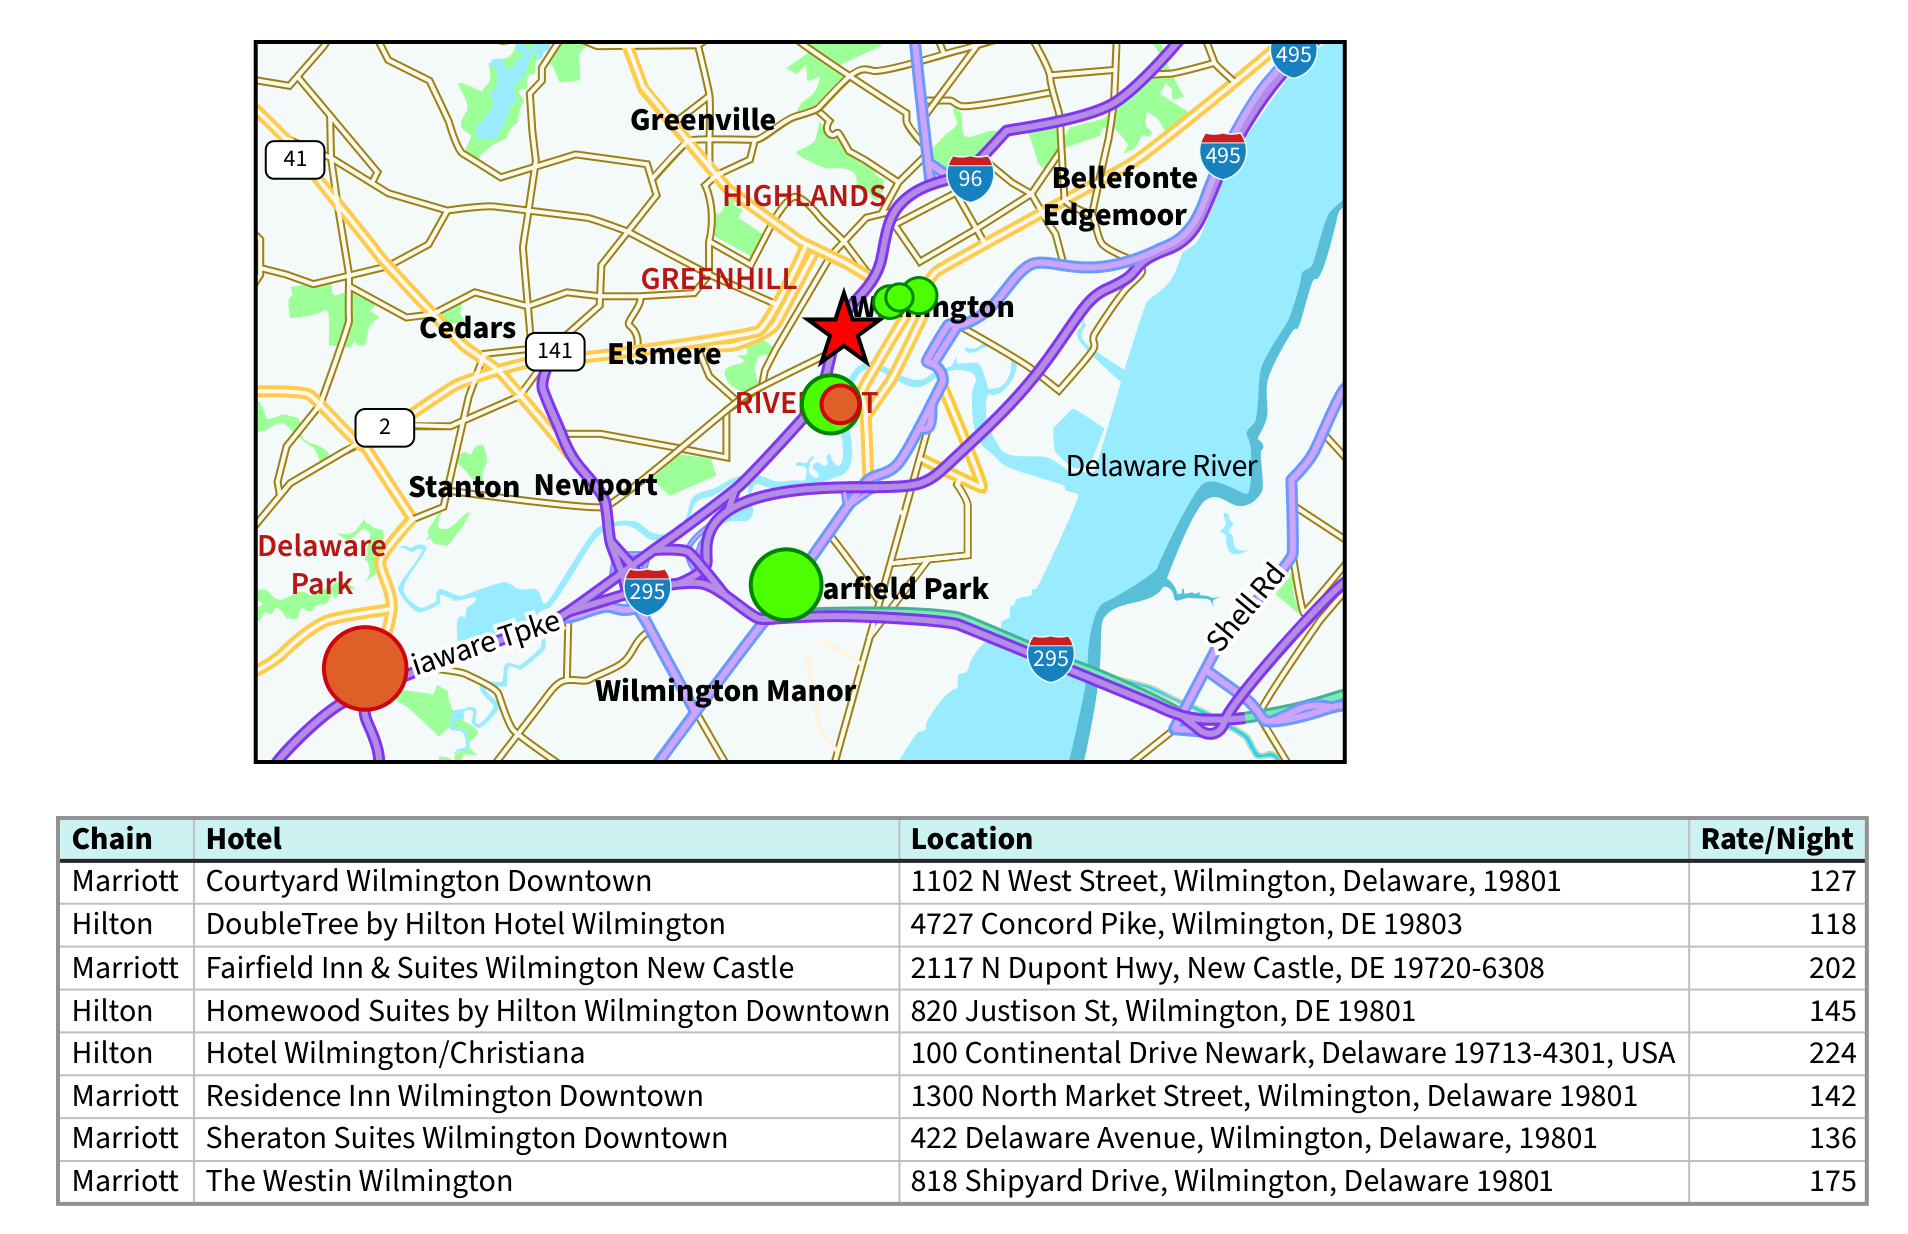
\includegraphics[width=\textwidth,height=0.7\textheight,keepaspectratio]{../textbookForPractice/Figures/Ch_07/EX 7.9.png}
            \end{figure}
        \end{column}
        \begin{column}{0.5\textwidth}
            \begin{figure}[h]
                \centering
                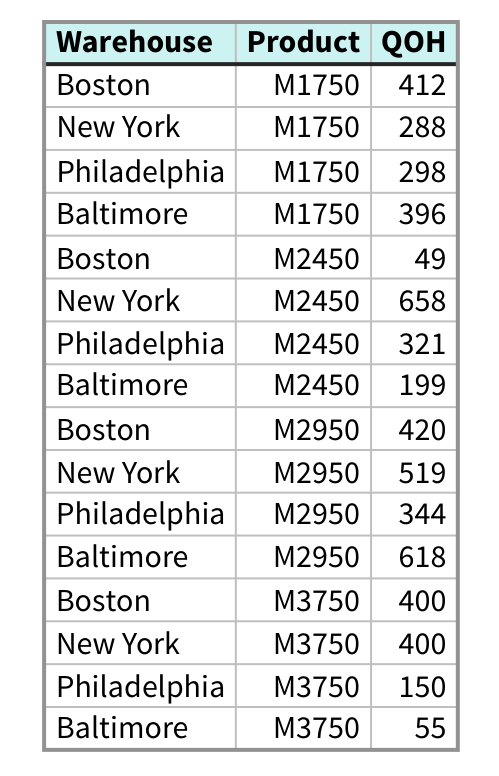
\includegraphics[width=\textwidth,height=0.7\textheight,keepaspectratio]{../textbookForPractice/Figures/Ch_07/EX 7.10A.png}
            \end{figure}
        \end{column}
    \end{columns}
\end{frame}

\begin{frame}{EX 7.10B \& EX 7.11}
    \begin{columns}
        \begin{column}{0.5\textwidth}
            \begin{figure}[h]
                \centering
                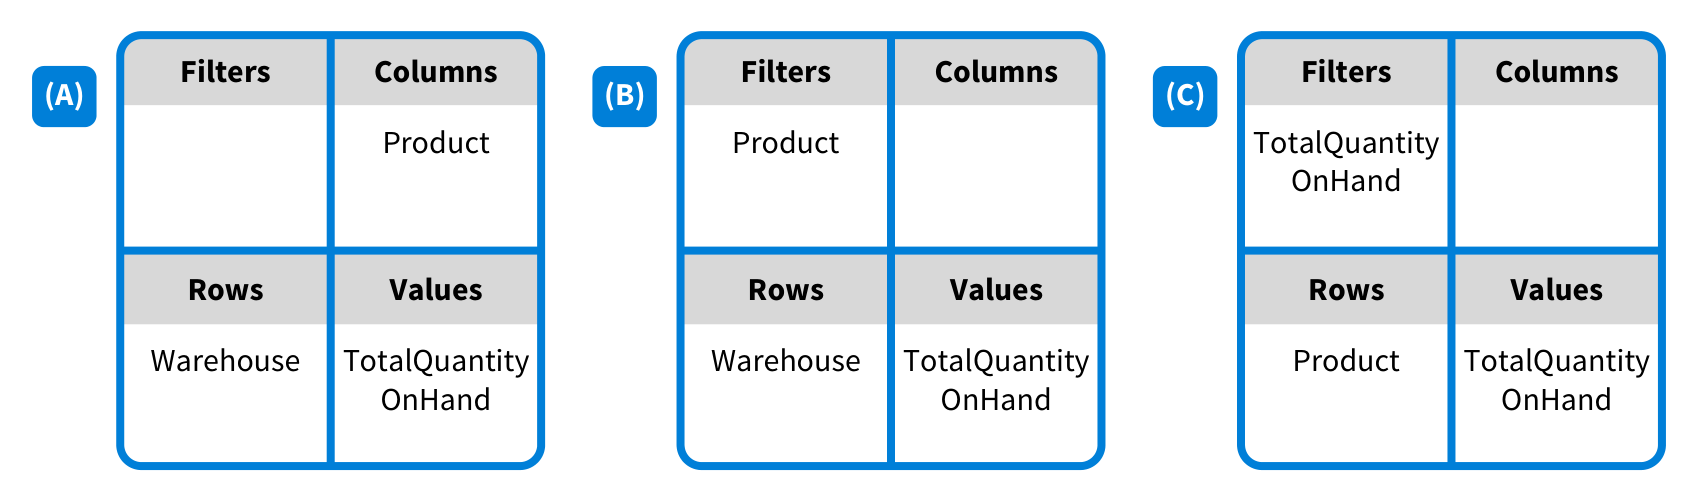
\includegraphics[width=\textwidth,height=0.7\textheight,keepaspectratio]{../textbookForPractice/Figures/Ch_07/EX 7.10B.png}
            \end{figure}
        \end{column}
        \begin{column}{0.5\textwidth}
            \begin{figure}[h]
                \centering
                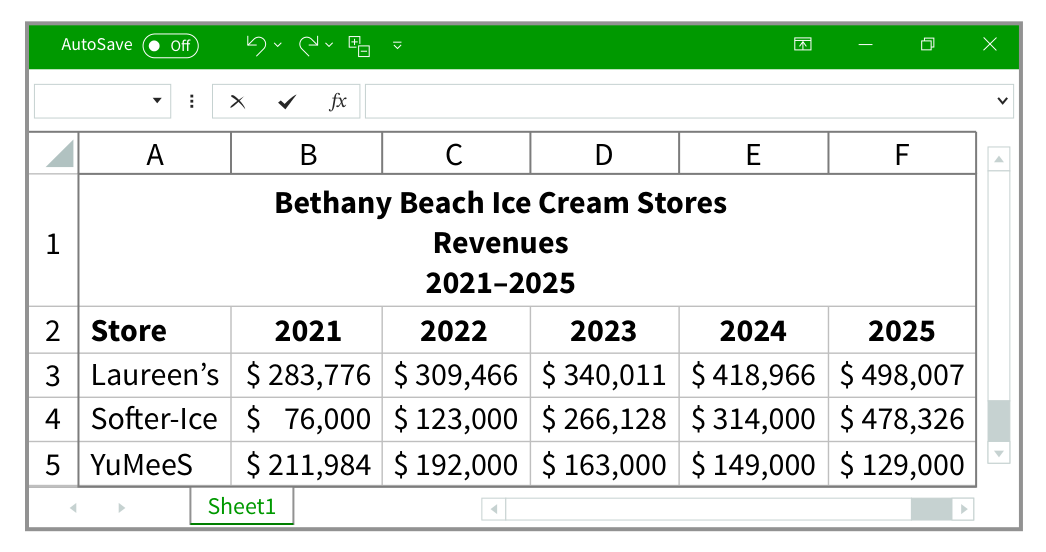
\includegraphics[width=\textwidth,height=0.7\textheight,keepaspectratio]{../textbookForPractice/Figures/Ch_07/EX 7.11.png}
            \end{figure}
        \end{column}
    \end{columns}
\end{frame}

\begin{frame}{EX 7.12 \& EX 7.13}
    \begin{columns}
        \begin{column}{0.5\textwidth}
            \begin{figure}[h]
                \centering
                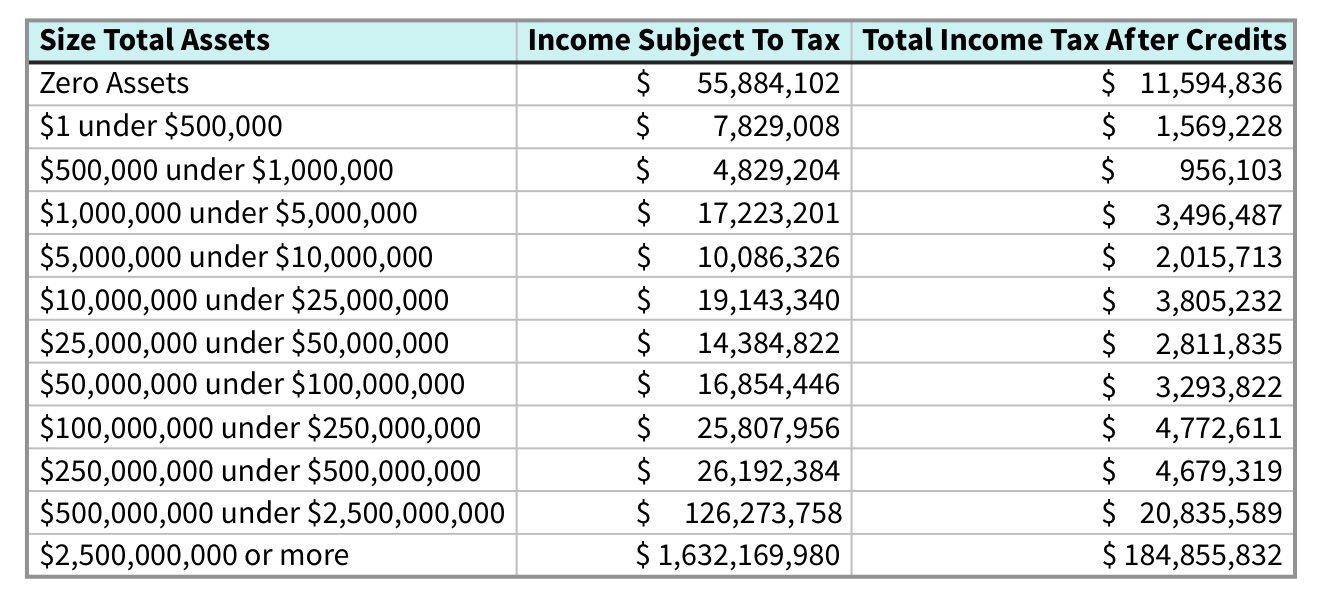
\includegraphics[width=\textwidth,height=0.7\textheight,keepaspectratio]{../textbookForPractice/Figures/Ch_07/EX 7.12.png}
            \end{figure}
        \end{column}
        \begin{column}{0.5\textwidth}
            \begin{figure}[h]
                \centering
                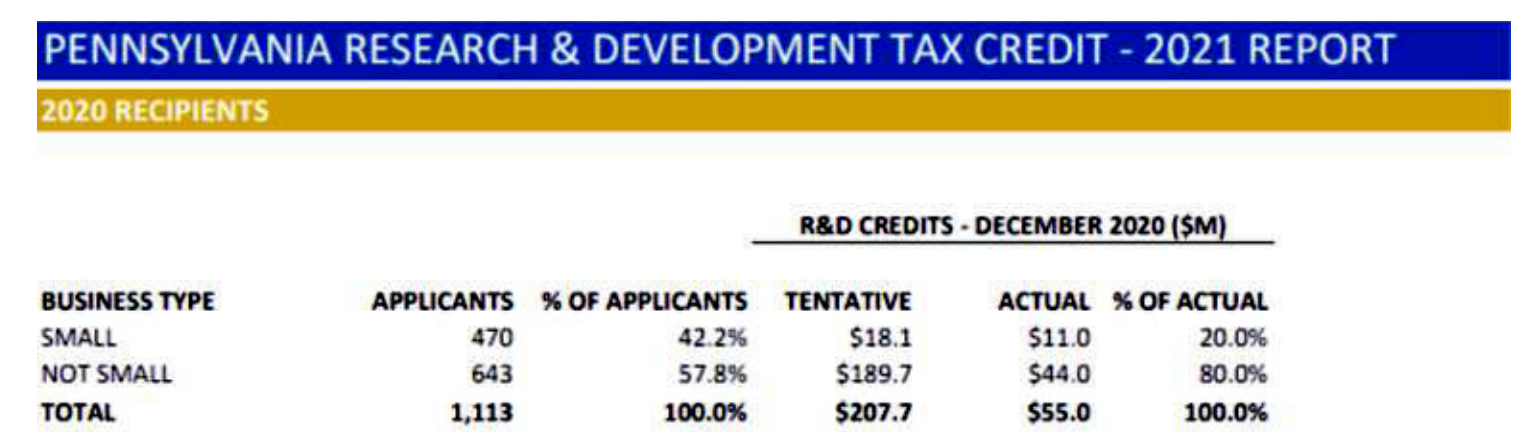
\includegraphics[width=\textwidth,height=0.7\textheight,keepaspectratio]{../textbookForPractice/Figures/Ch_07/EX 7.13.png}
            \end{figure}
        \end{column}
    \end{columns}
\end{frame}

\begin{frame}{EX 7.14 \& EX 7.15}
    \begin{columns}
        \begin{column}{0.5\textwidth}
            \begin{figure}[h]
                \centering
                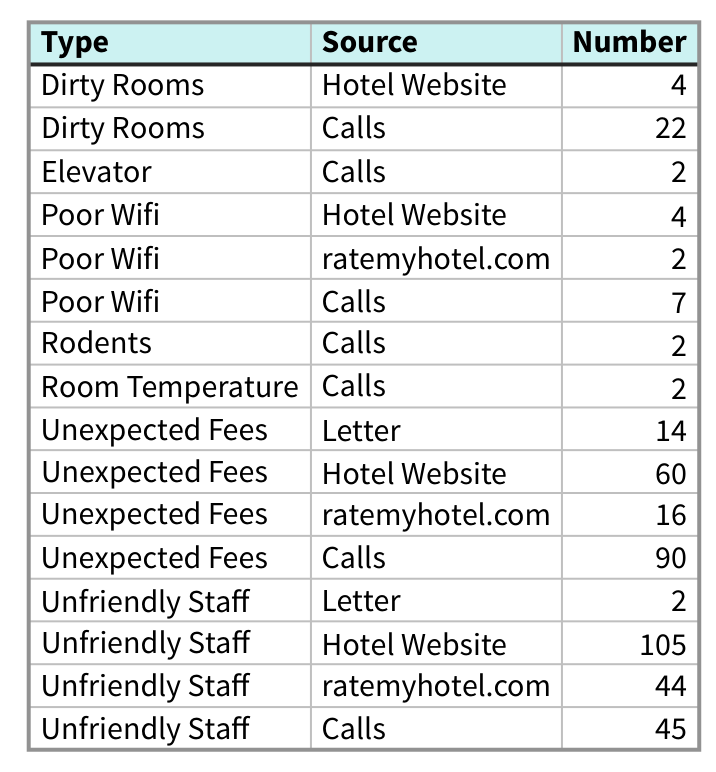
\includegraphics[width=\textwidth,height=0.7\textheight,keepaspectratio]{../textbookForPractice/Figures/Ch_07/EX 7.14.png}
            \end{figure}
        \end{column}
        \begin{column}{0.5\textwidth}
            \begin{figure}[h]
                \centering
                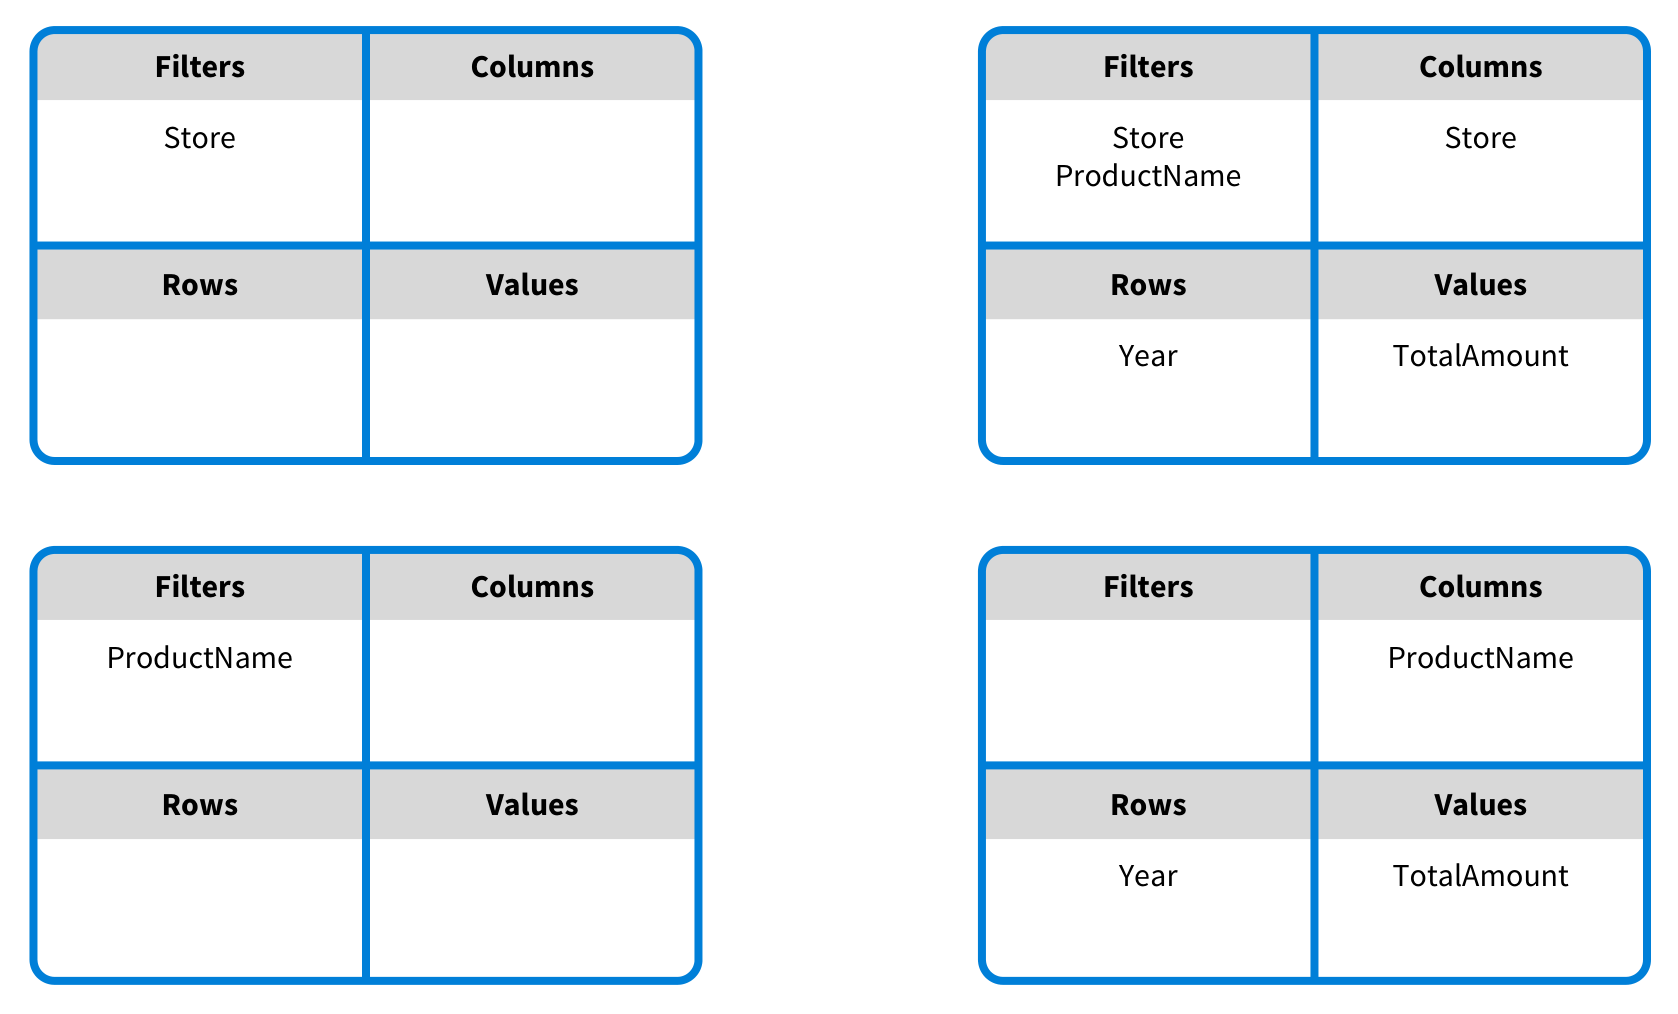
\includegraphics[width=\textwidth,height=0.7\textheight,keepaspectratio]{../textbookForPractice/Figures/Ch_07/EX 7.15.png}
            \end{figure}
        \end{column}
    \end{columns}
\end{frame}

\begin{frame}{LO 2.10}

    \begin{figure}[h]
        \centering
        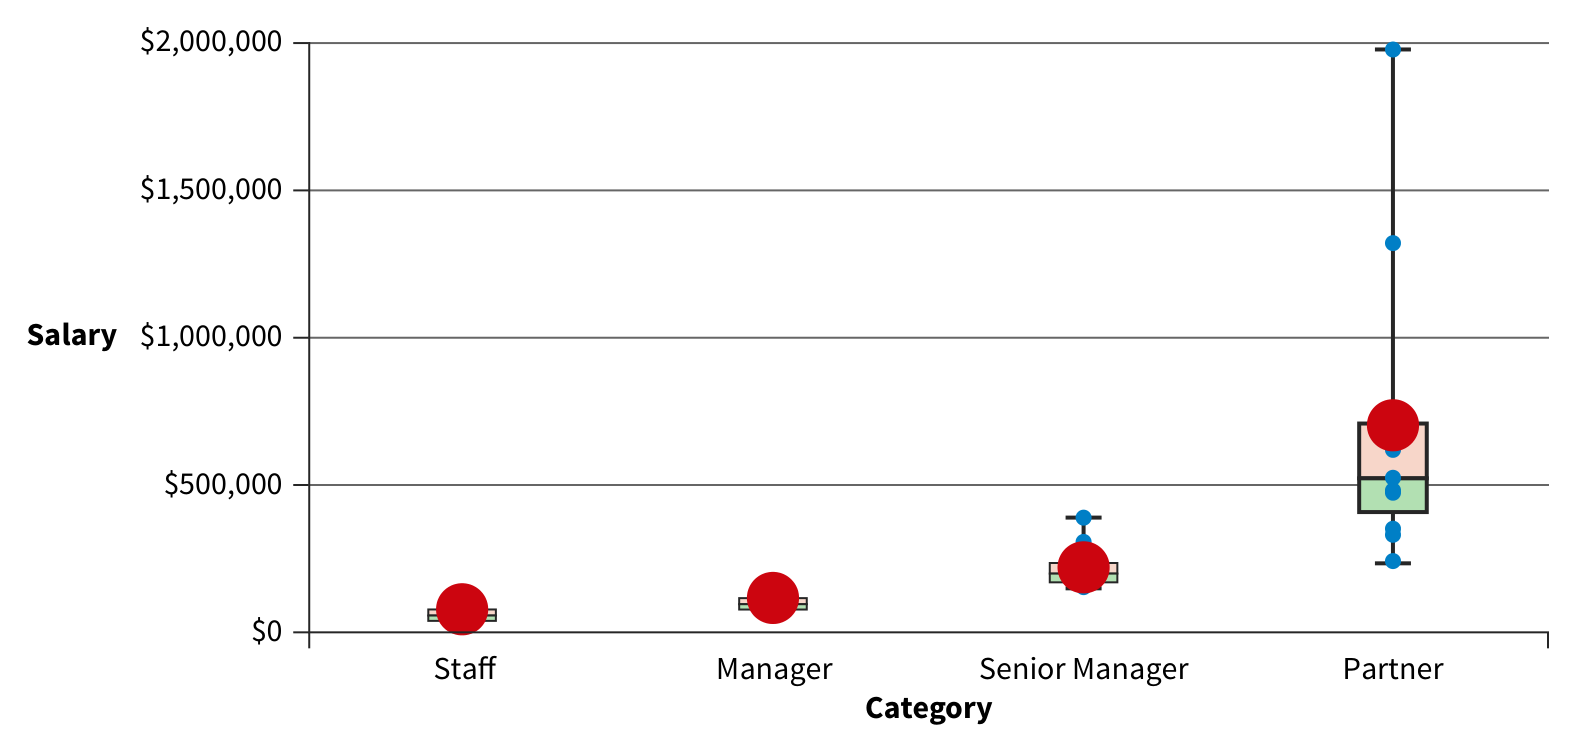
\includegraphics[width=0.95\textwidth,height=0.75\textheight,keepaspectratio]{../textbookForPractice/Figures/Ch_07/LO 2.10.png}
    \end{figure}
\end{frame}

\begin{frame}{LO 2.11}

    \begin{figure}[h]
        \centering
        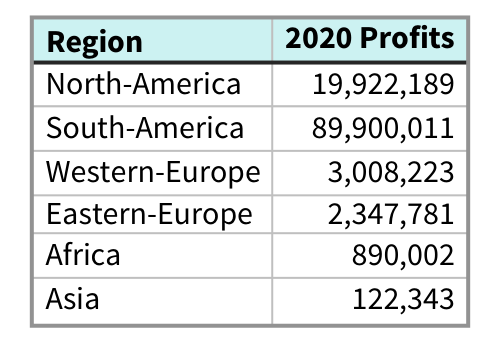
\includegraphics[width=0.95\textwidth,height=0.75\textheight,keepaspectratio]{../textbookForPractice/Figures/Ch_07/LO 2.11.png}
    \end{figure}
\end{frame}

\begin{frame}{LO 2.14}

    \begin{figure}[h]
        \centering
        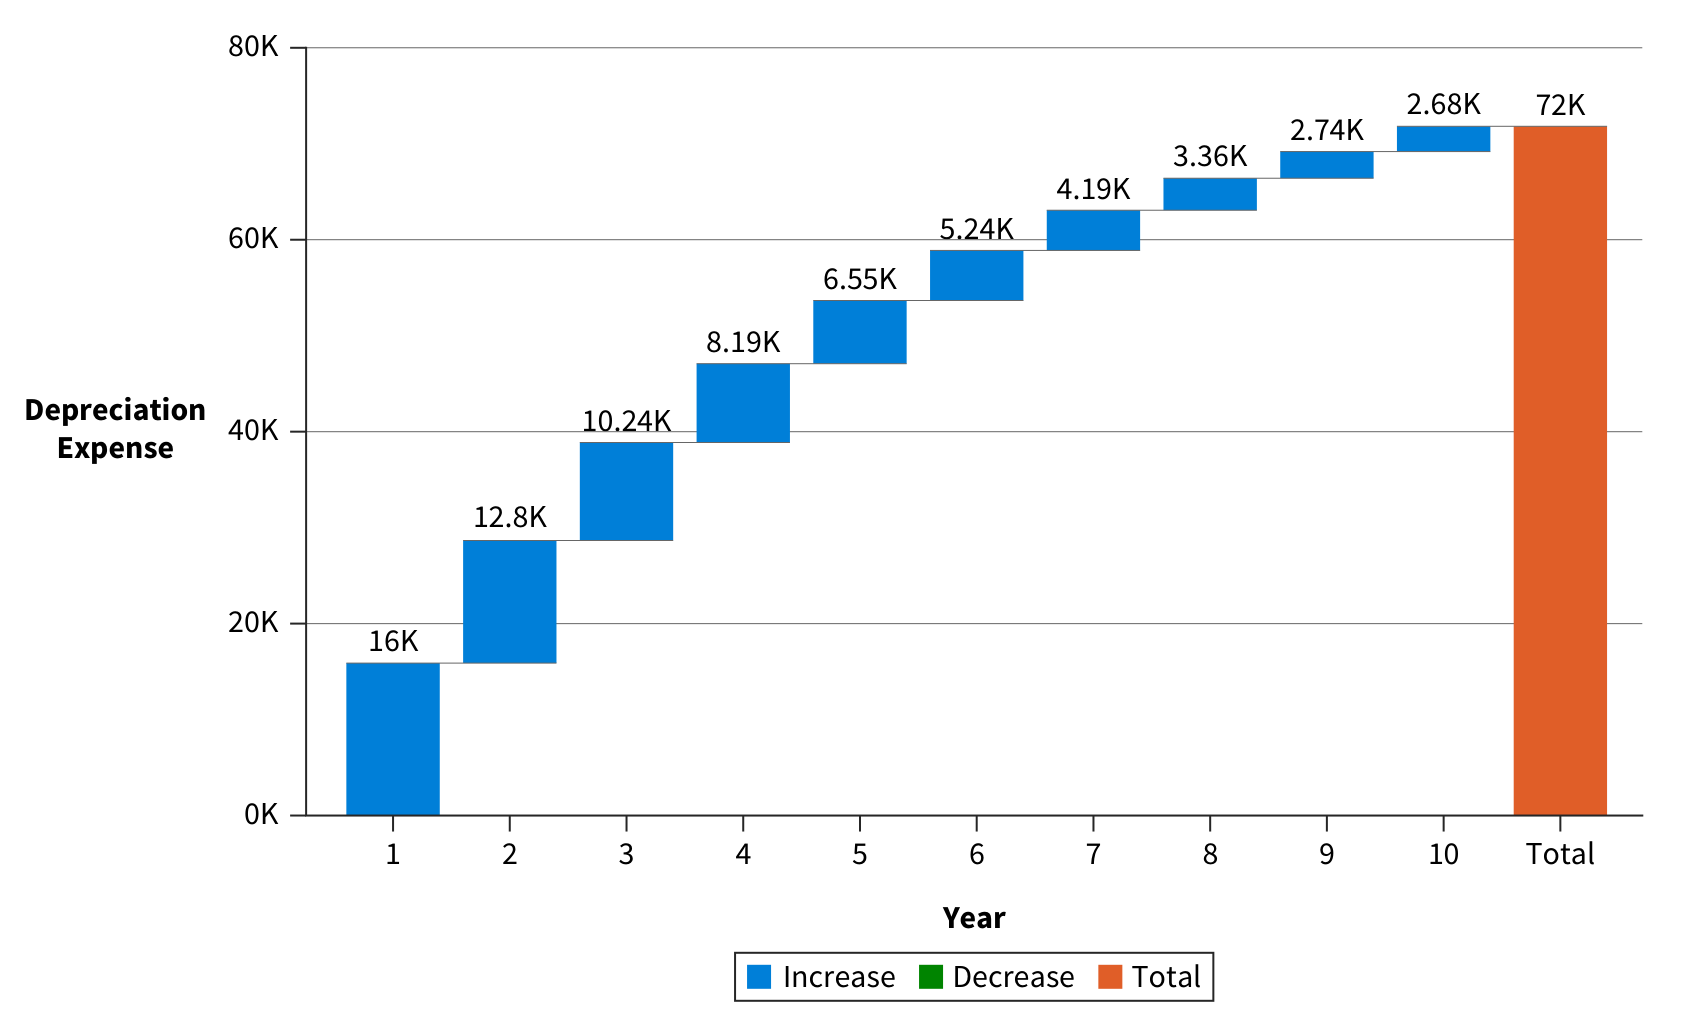
\includegraphics[width=0.95\textwidth,height=0.75\textheight,keepaspectratio]{../textbookForPractice/Figures/Ch_07/LO 2.14.png}
    \end{figure}
\end{frame}

\begin{frame}{LO 2.14\_1}

    \begin{figure}[h]
        \centering
        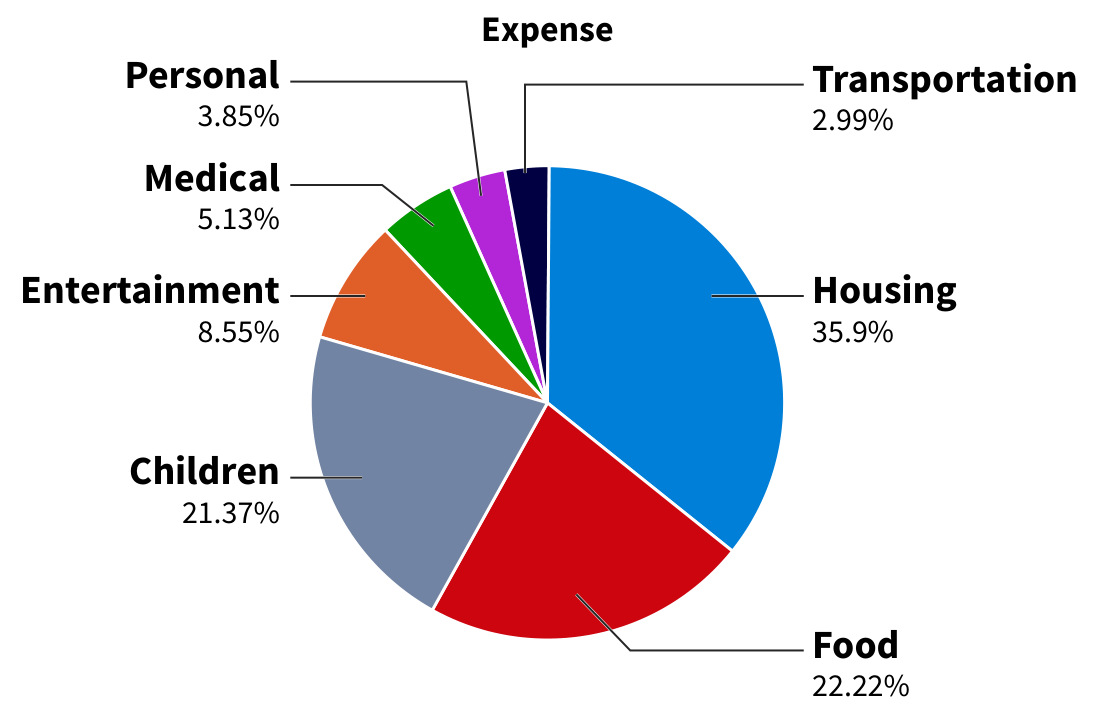
\includegraphics[width=0.95\textwidth,height=0.75\textheight,keepaspectratio]{../textbookForPractice/Figures/Ch_07/LO 2.14_1.png}
    \end{figure}
\end{frame}

\begin{frame}{LO 2.15}

    \begin{figure}[h]
        \centering
        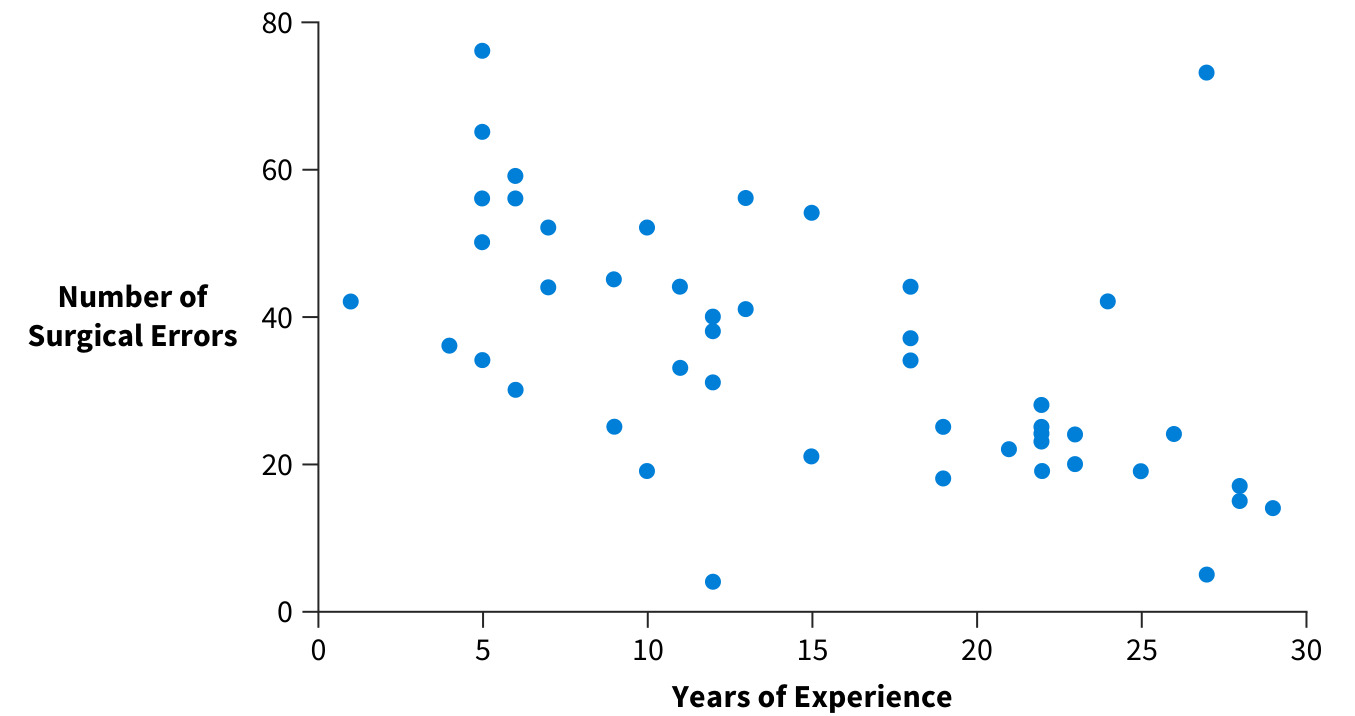
\includegraphics[width=0.95\textwidth,height=0.75\textheight,keepaspectratio]{../textbookForPractice/Figures/Ch_07/LO 2.15.png}
    \end{figure}
\end{frame}

\begin{frame}{LO 3.15}

    \begin{figure}[h]
        \centering
        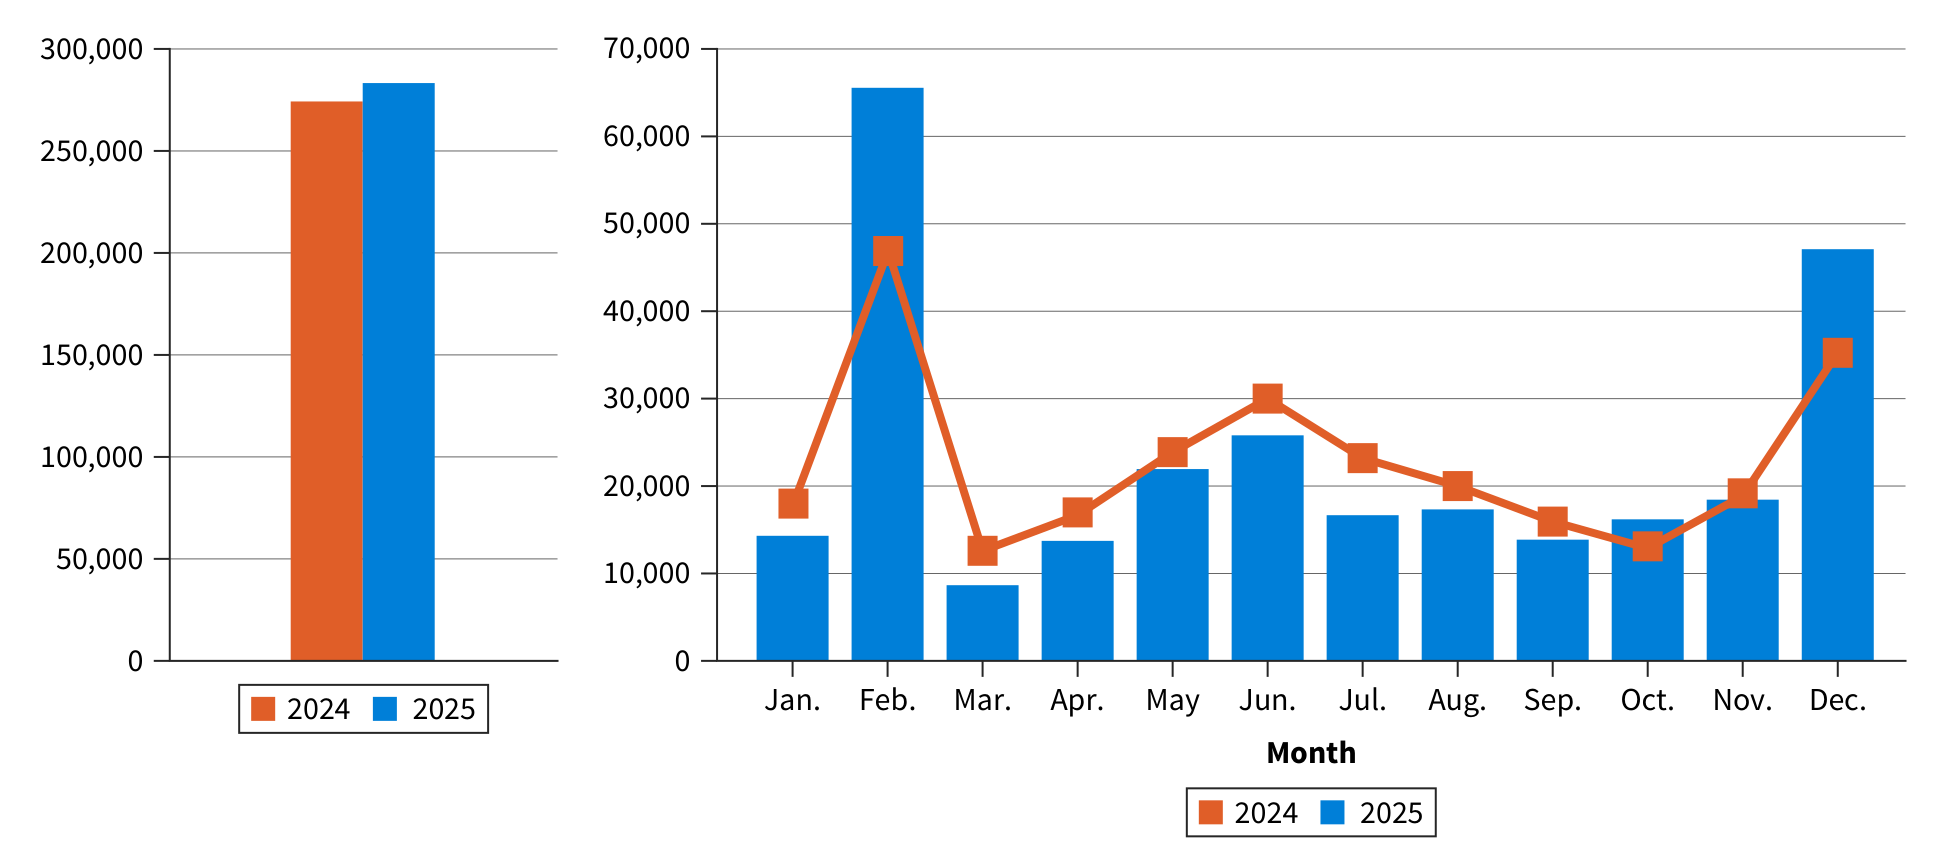
\includegraphics[width=0.95\textwidth,height=0.75\textheight,keepaspectratio]{../textbookForPractice/Figures/Ch_07/LO 3.15.png}
    \end{figure}
\end{frame}

\begin{frame}{LO 3.16}

    \begin{figure}[h]
        \centering
        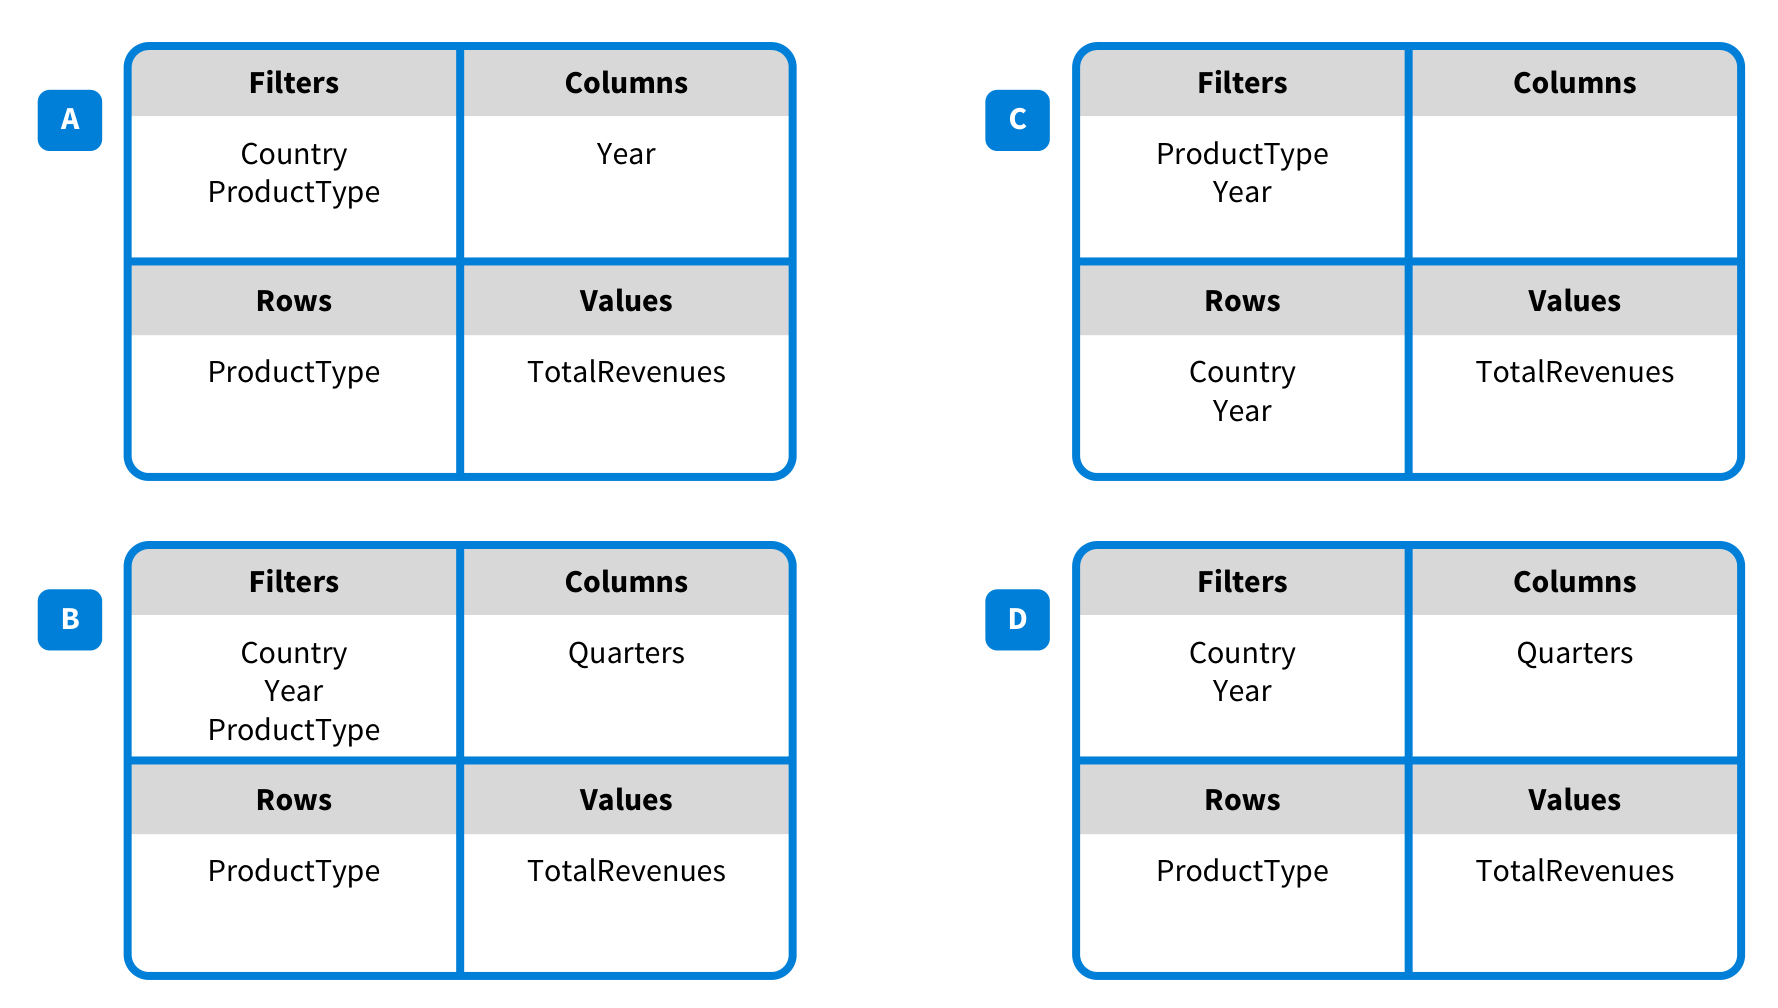
\includegraphics[width=0.95\textwidth,height=0.75\textheight,keepaspectratio]{../textbookForPractice/Figures/Ch_07/LO 3.16.png}
    \end{figure}
\end{frame}

\begin{frame}{LO 3.17}

    \begin{figure}[h]
        \centering
        
\includegraphics[width=0.95\textwidth,height=0.75\textheight,keepaspectratio]{../textbookForPractice/Figures/Ch_07/LO 3.17.png}
    \end{figure}
\end{frame}

\begin{frame}{LO 3.18}

    \begin{figure}[h]
        \centering
        
\includegraphics[width=0.95\textwidth,height=0.75\textheight,keepaspectratio]{../textbookForPractice/Figures/Ch_07/LO 3.18.png}
    \end{figure}
\end{frame}

\begin{frame}{LO 3.19}

    \begin{figure}[h]
        \centering
        
\includegraphics[width=0.95\textwidth,height=0.75\textheight,keepaspectratio]{../textbookForPractice/Figures/Ch_07/LO 3.19.png}
    \end{figure}
\end{frame}

\begin{frame}{LO 3.20A}

    \begin{figure}[h]
        \centering
        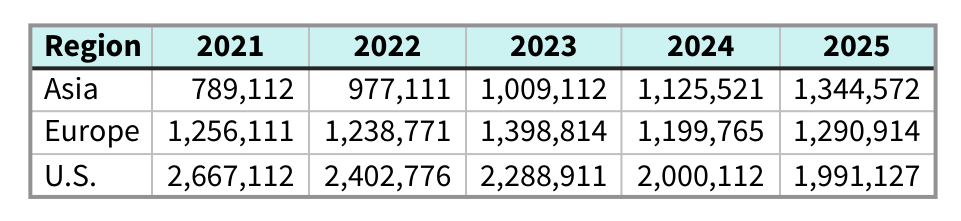
\includegraphics[width=0.95\textwidth,height=0.75\textheight,keepaspectratio]{../textbookForPractice/Figures/Ch_07/LO 3.20A.png}
    \end{figure}
\end{frame}

\begin{frame}{LO 3.20B}

    \begin{figure}[h]
        \centering
        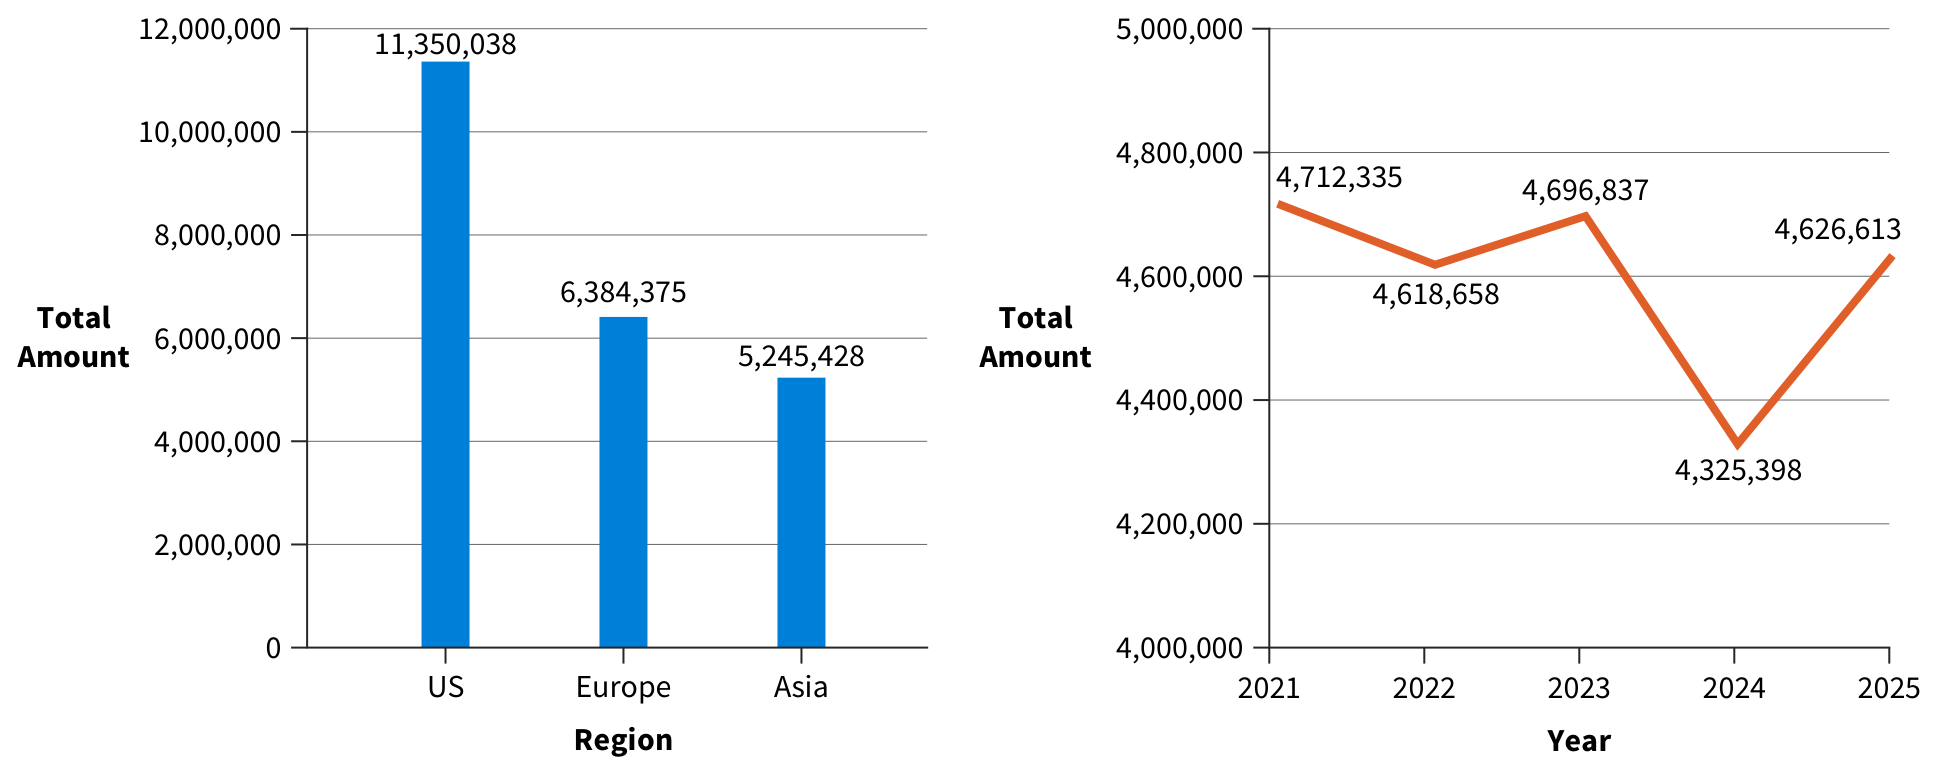
\includegraphics[width=0.95\textwidth,height=0.75\textheight,keepaspectratio]{../textbookForPractice/Figures/Ch_07/LO 3.20B.png}
    \end{figure}
\end{frame}

\begin{frame}{LO 3.20C}

    \begin{figure}[h]
        \centering
        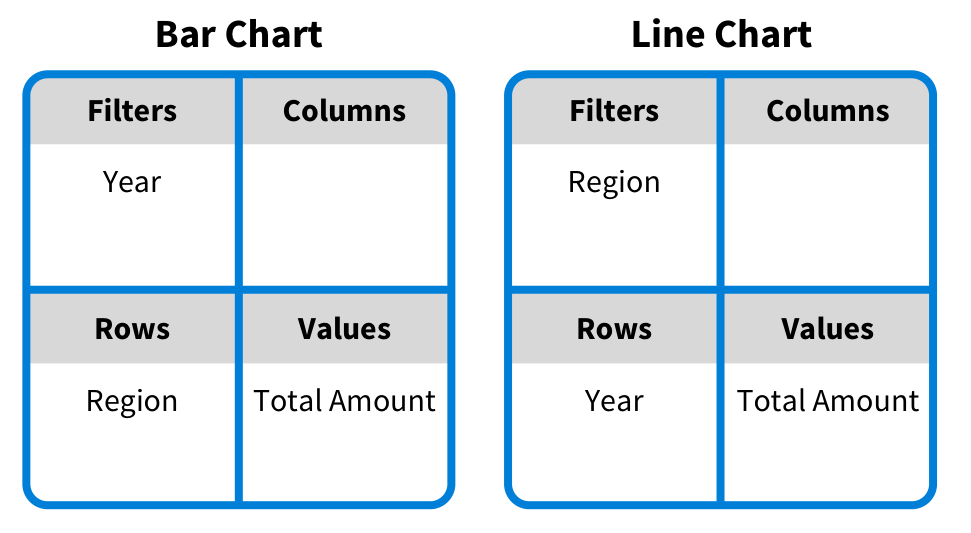
\includegraphics[width=0.95\textwidth,height=0.75\textheight,keepaspectratio]{../textbookForPractice/Figures/Ch_07/LO 3.20C.png}
    \end{figure}
\end{frame}

\begin{frame}{LO 3.20A\_1}

    \begin{figure}[h]
        \centering
        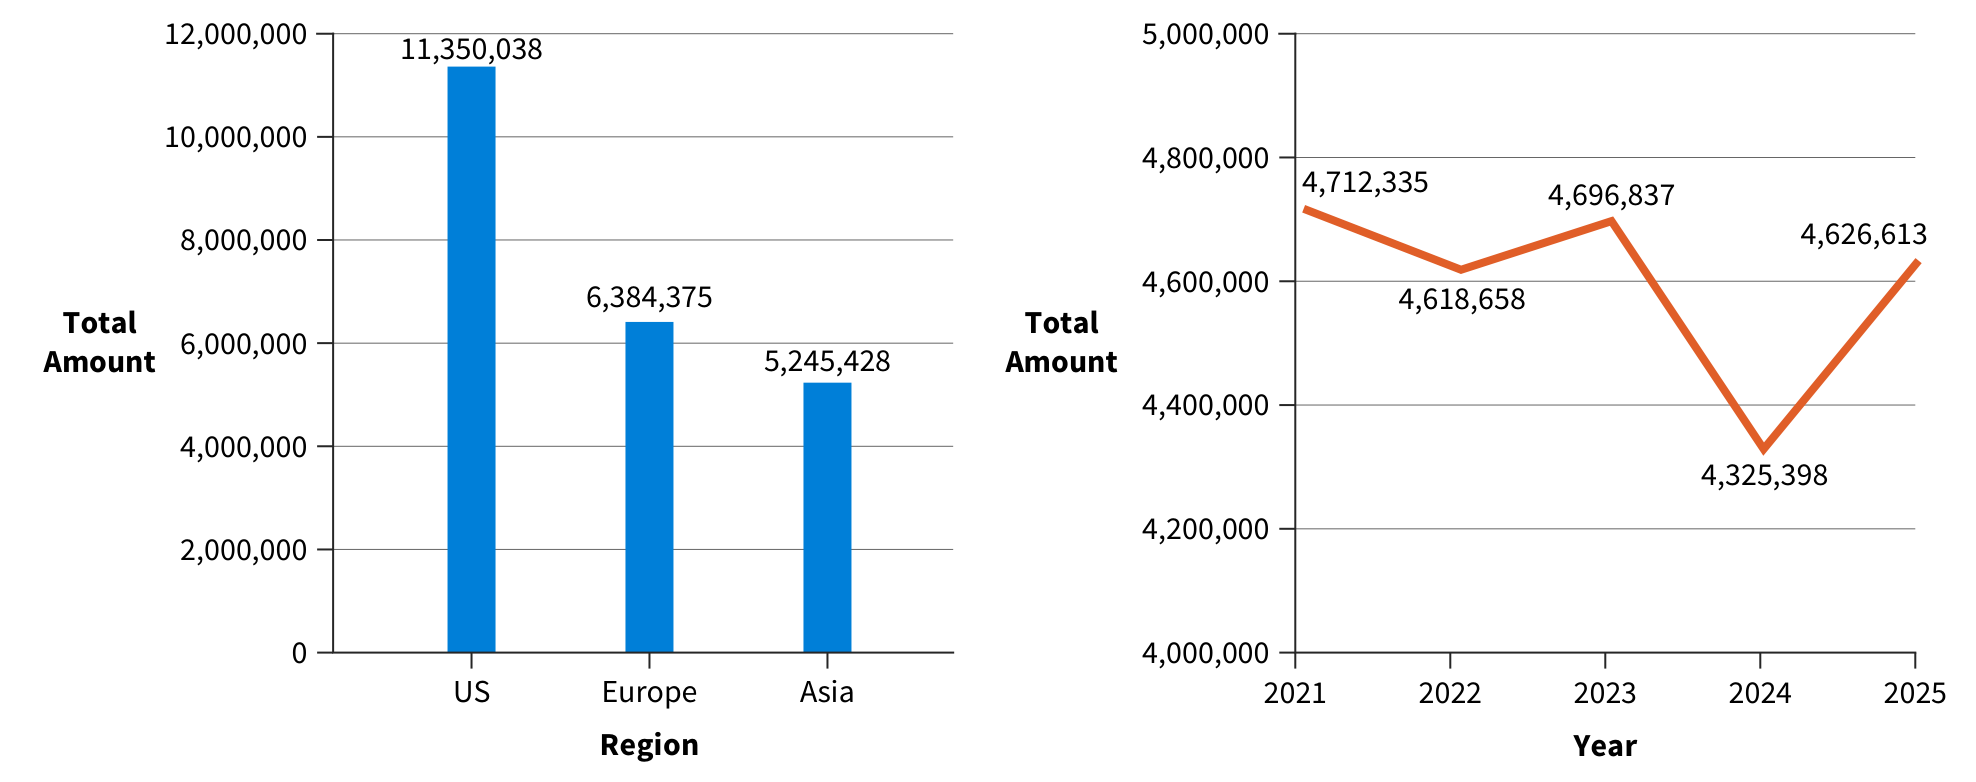
\includegraphics[width=0.95\textwidth,height=0.75\textheight,keepaspectratio]{../textbookForPractice/Figures/Ch_07/LO 3.20A_1.png}
    \end{figure}
\end{frame}

\begin{frame}{LO 3.20A\_2}

    \begin{figure}[h]
        \centering
        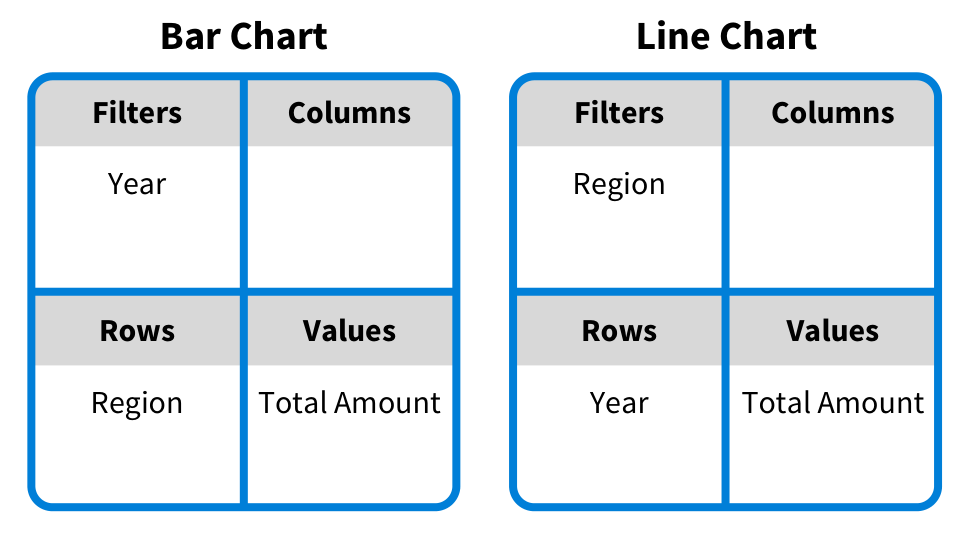
\includegraphics[width=0.95\textwidth,height=0.75\textheight,keepaspectratio]{../textbookForPractice/Figures/Ch_07/LO 3.20A_2.png}
    \end{figure}
\end{frame}

\begin{frame}{Info 7.0}

    \begin{figure}[h]
        \centering
        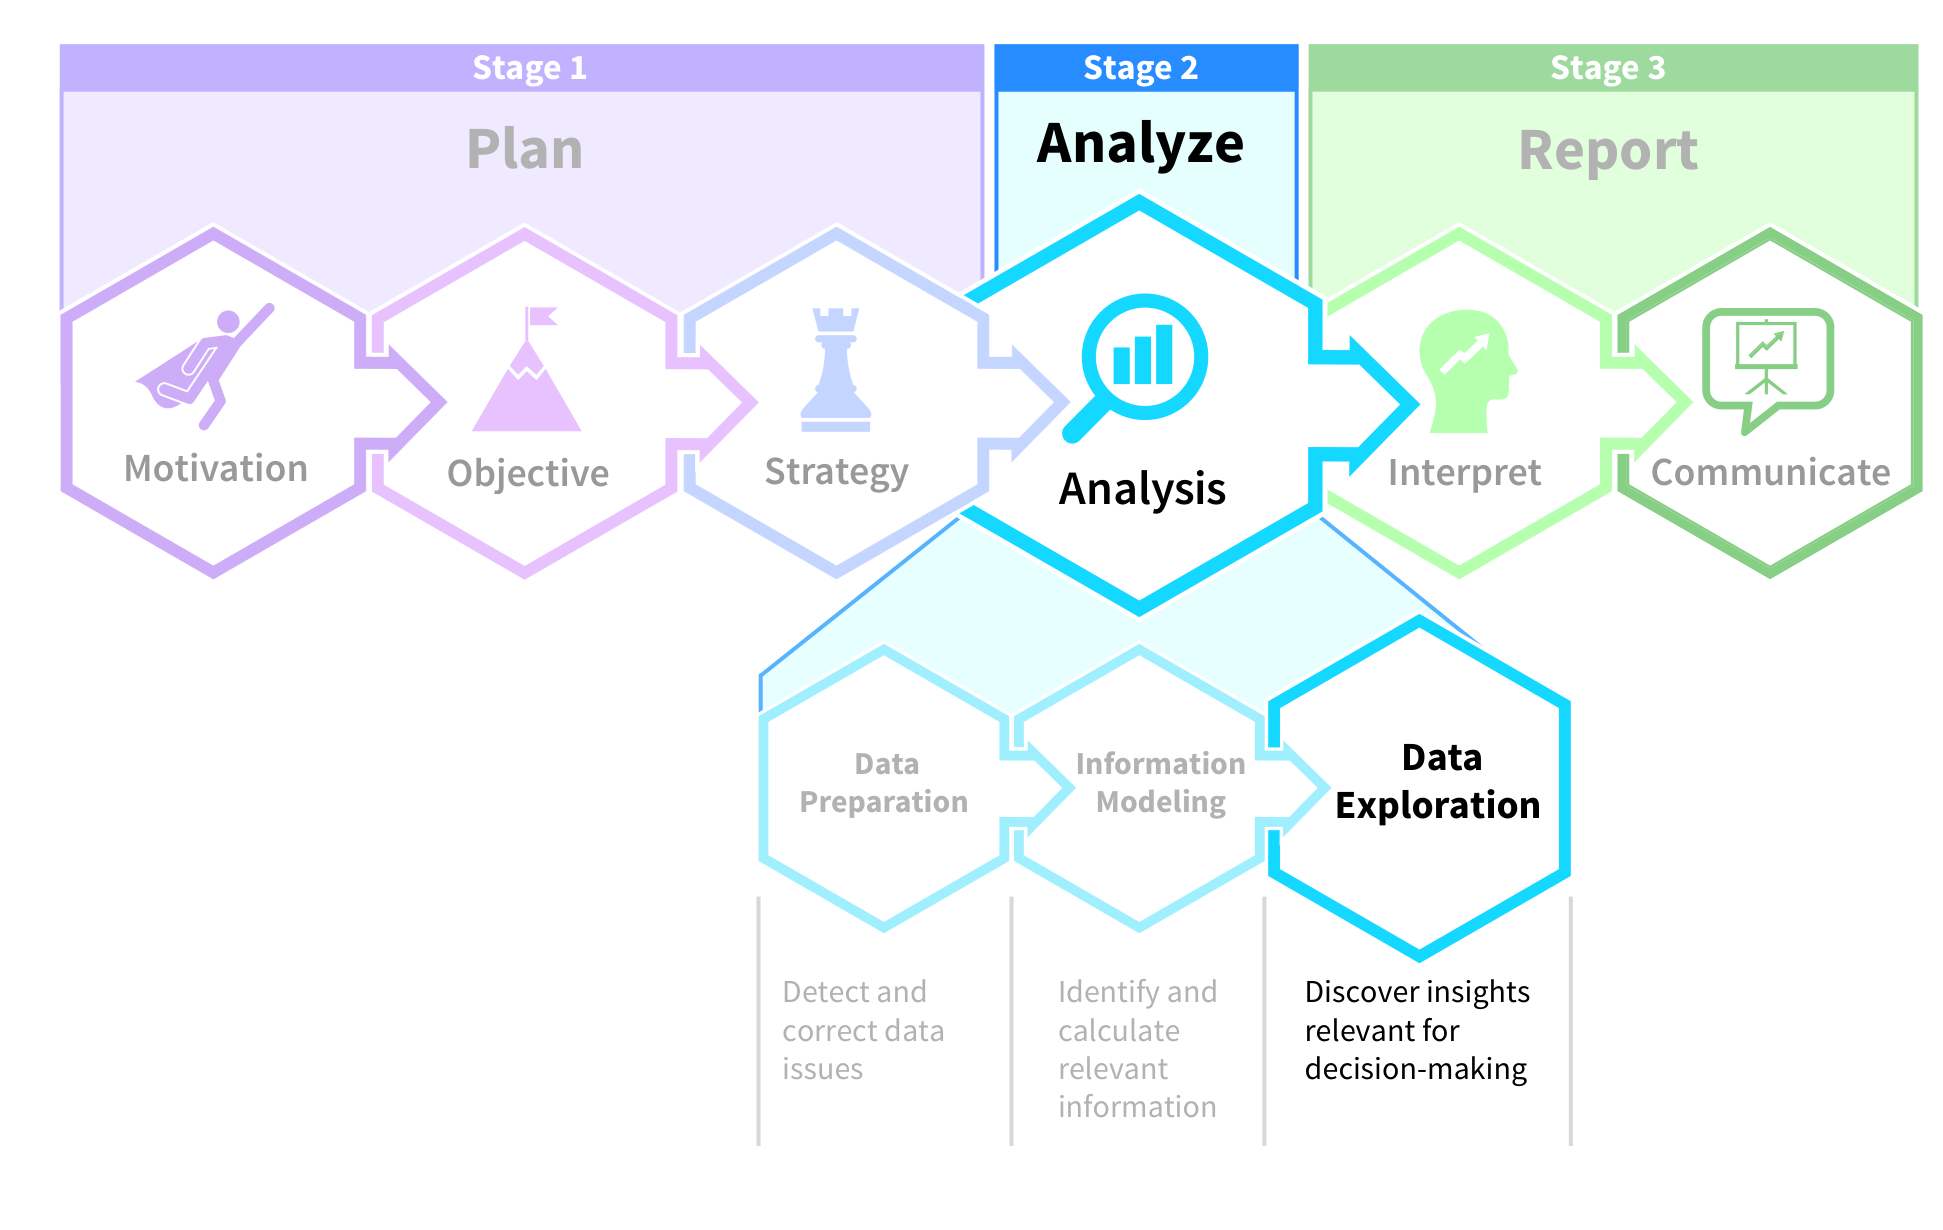
\includegraphics[width=0.95\textwidth,height=0.75\textheight,keepaspectratio]{../textbookForPractice/Figures/Ch_07/Info 7.0.png}
    \end{figure}
\end{frame}

\begin{frame}{Apply It 7.1A}

    \begin{figure}[h]
        \centering
        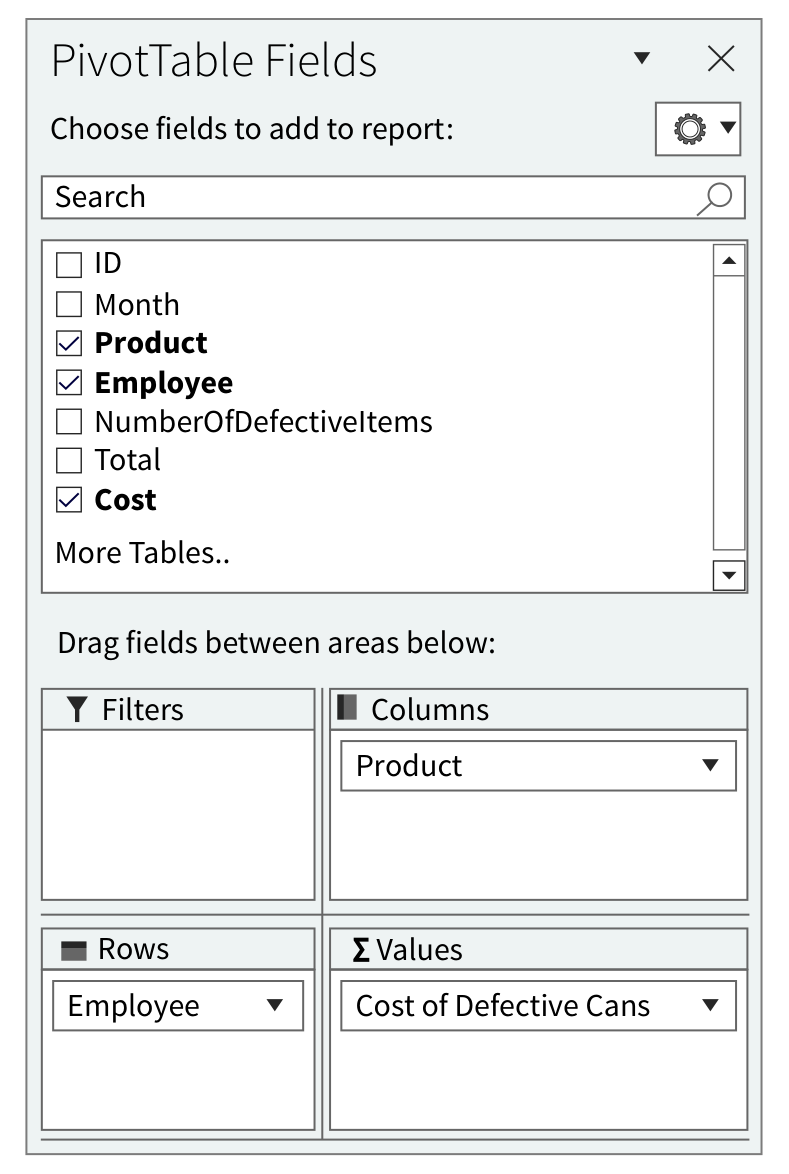
\includegraphics[width=0.95\textwidth,height=0.75\textheight,keepaspectratio]{../textbookForPractice/Figures/Ch_07/Apply It 7.1A.png}
    \end{figure}
\end{frame}

\begin{frame}{Apply It 7.1B}

    \begin{figure}[h]
        \centering
        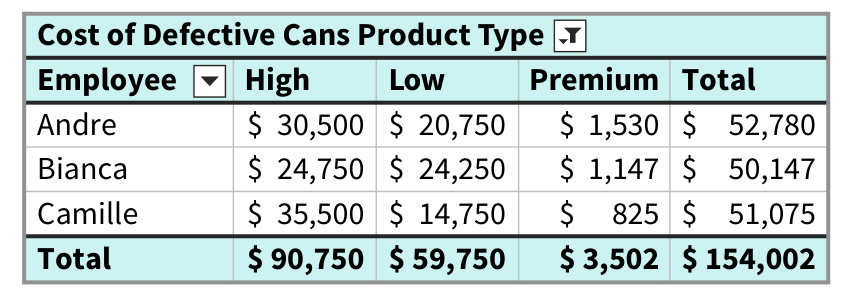
\includegraphics[width=0.95\textwidth,height=0.75\textheight,keepaspectratio]{../textbookForPractice/Figures/Ch_07/Apply It 7.1B.png}
    \end{figure}
\end{frame}

\begin{frame}{Apply It 7.2}

    \begin{figure}[h]
        \centering
        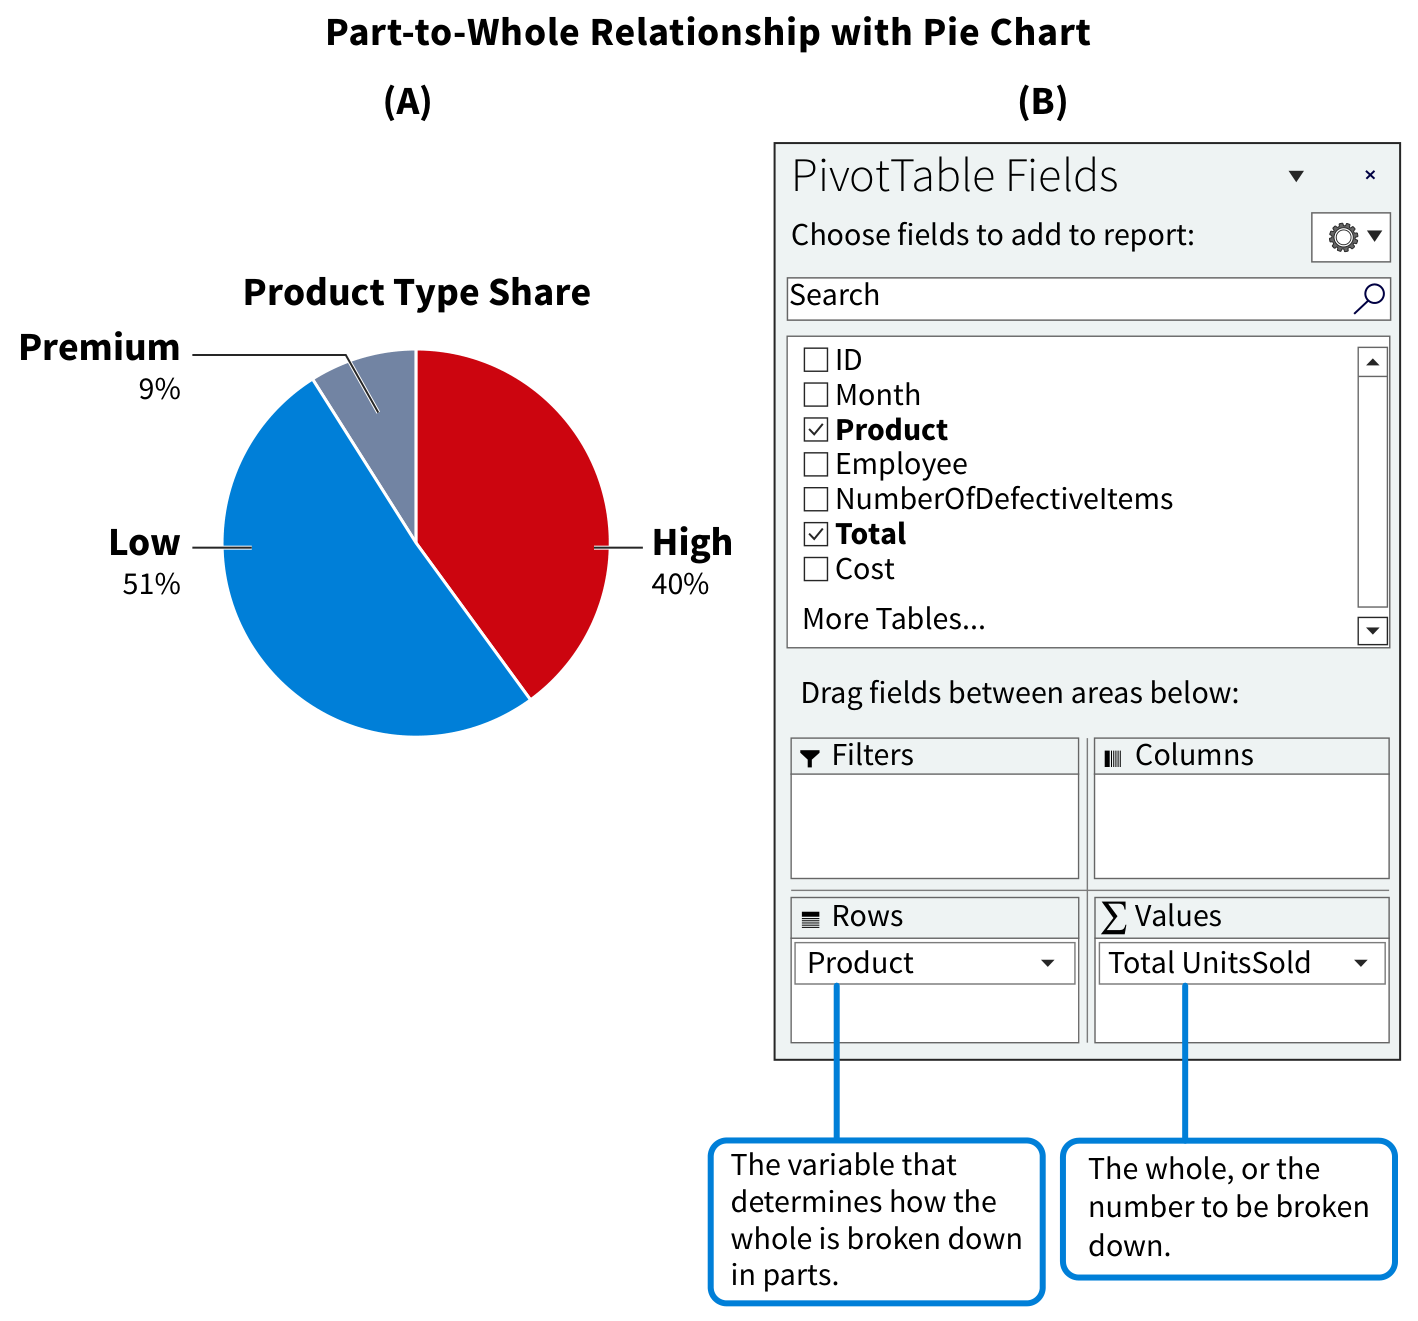
\includegraphics[width=0.95\textwidth,height=0.75\textheight,keepaspectratio]{../textbookForPractice/Figures/Ch_07/Apply It 7.2.png}
    \end{figure}
\end{frame}

\begin{frame}{Apply It 7.3A}

    \begin{figure}[h]
        \centering
        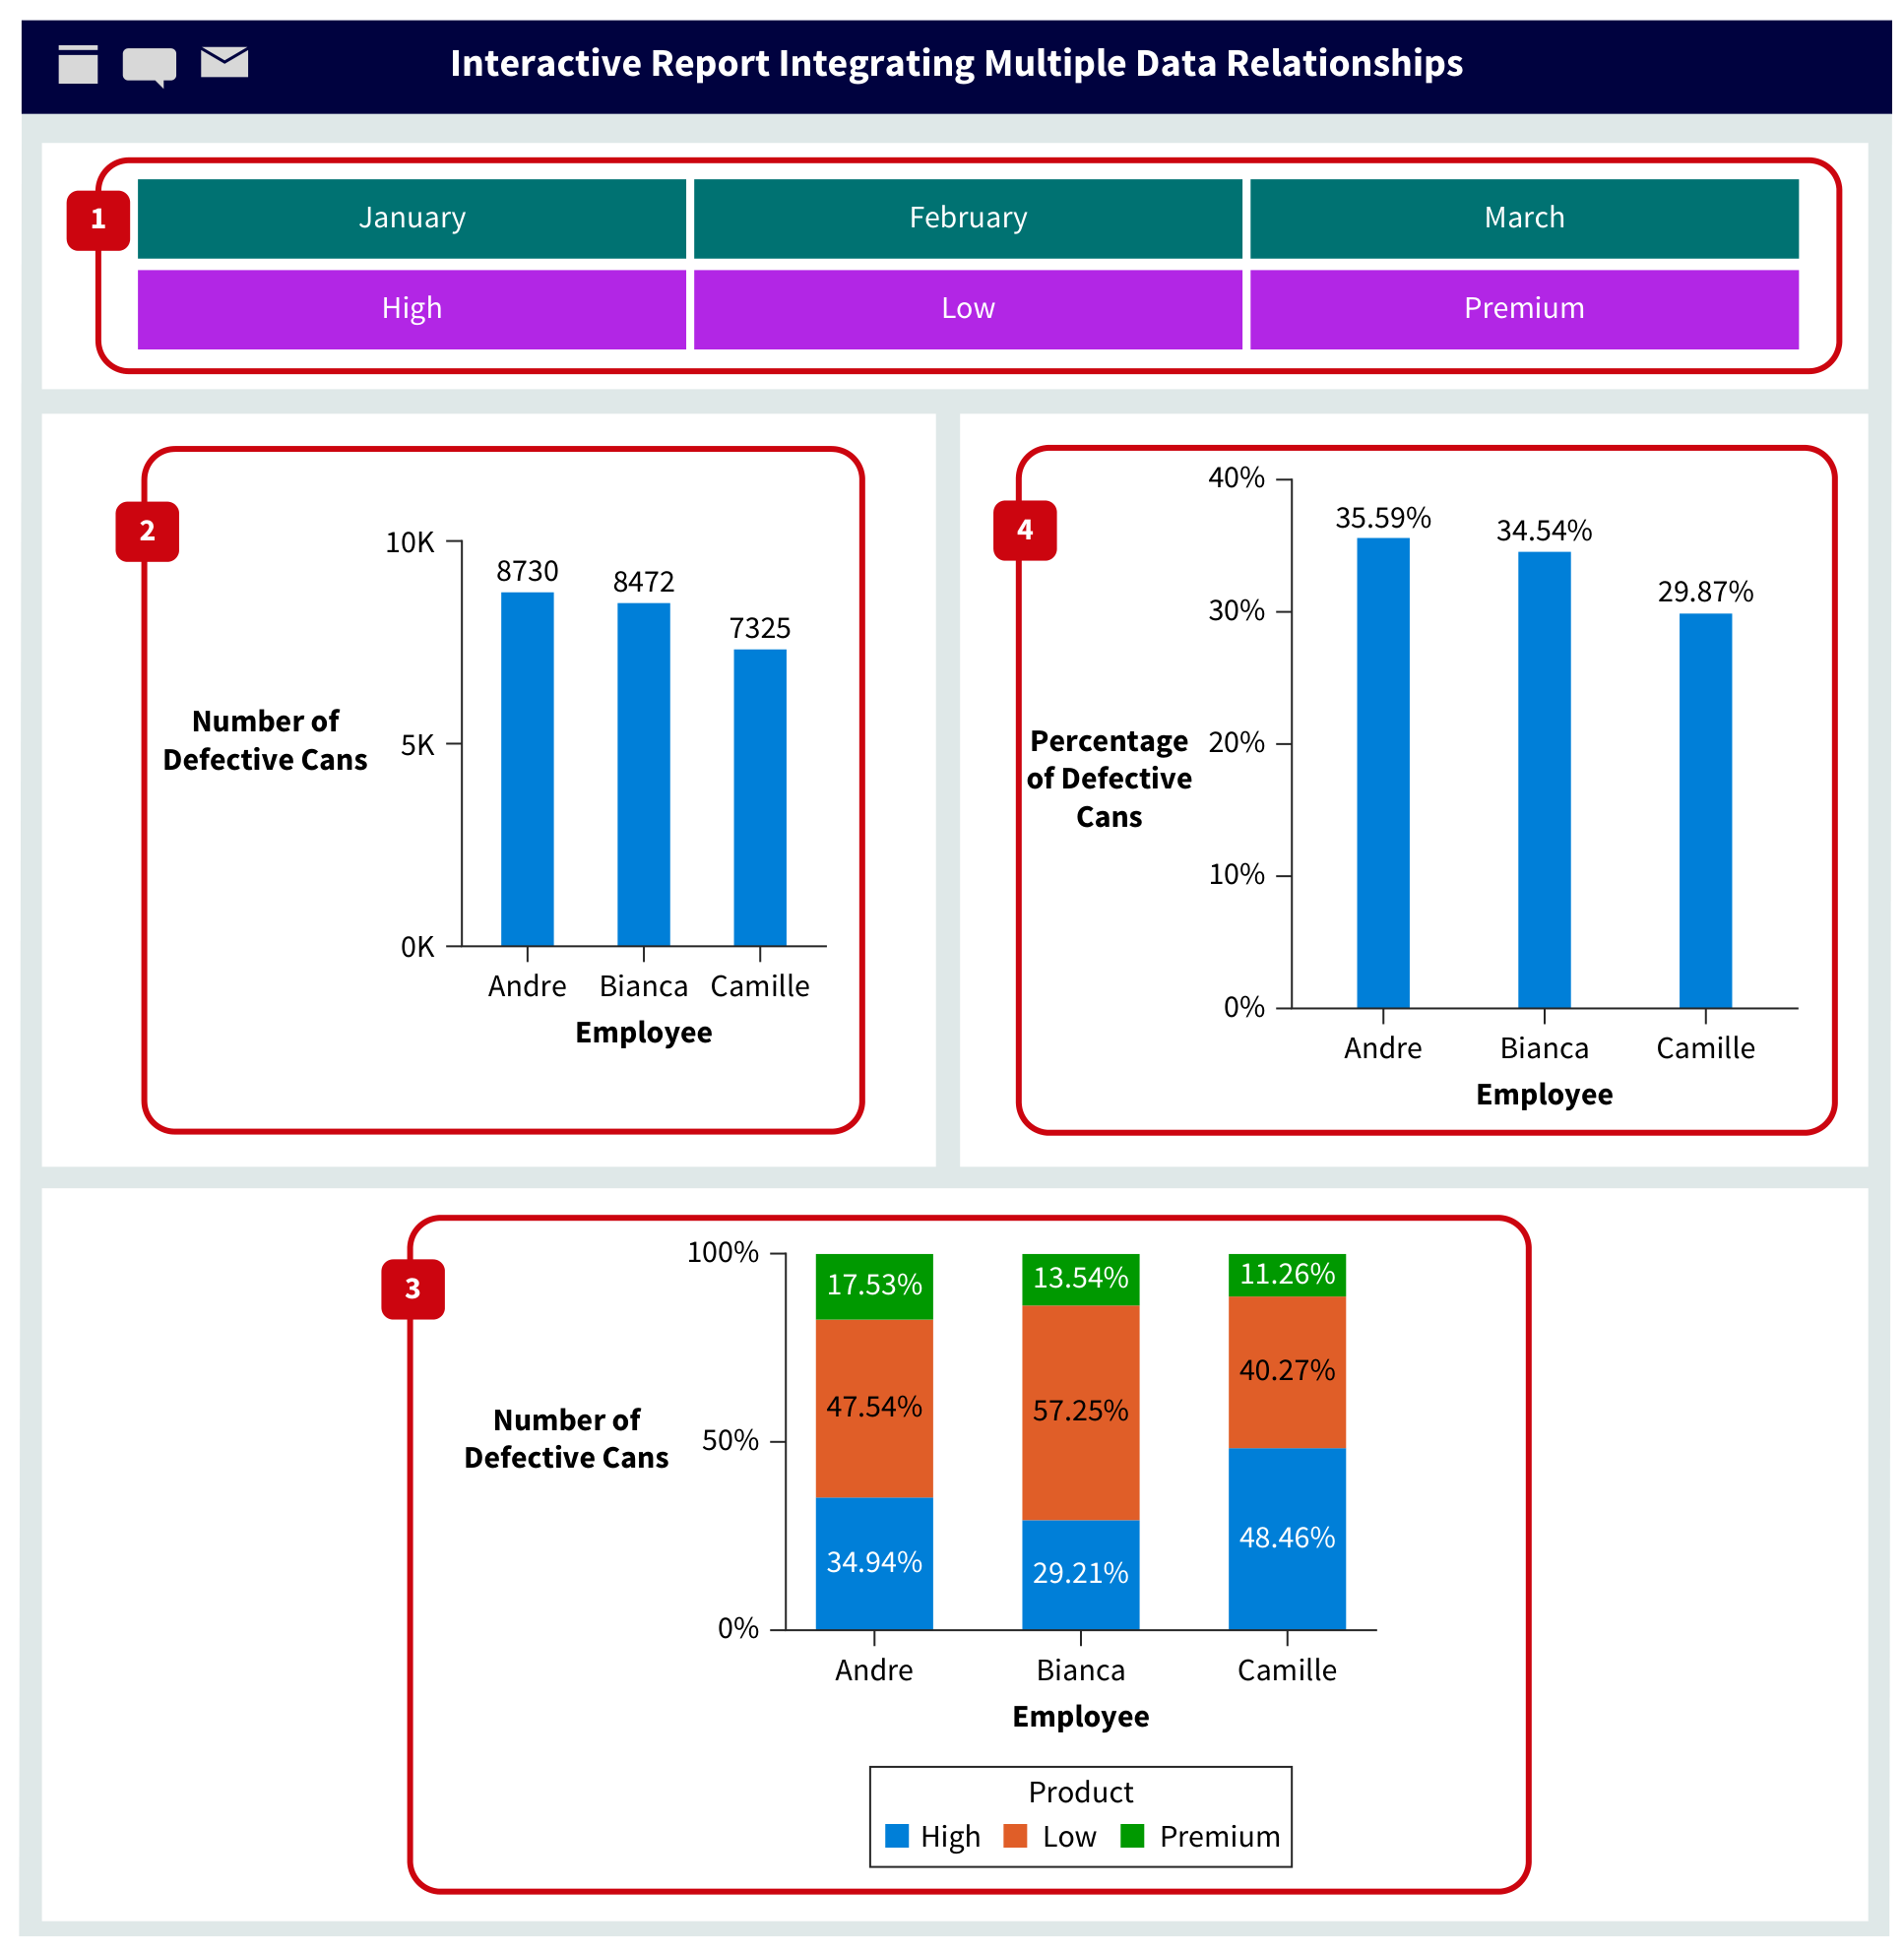
\includegraphics[width=0.95\textwidth,height=0.75\textheight,keepaspectratio]{../textbookForPractice/Figures/Ch_07/Apply It 7.3A.png}
    \end{figure}
\end{frame}

\begin{frame}{Apply It 7.3B}

    \begin{figure}[h]
        \centering
        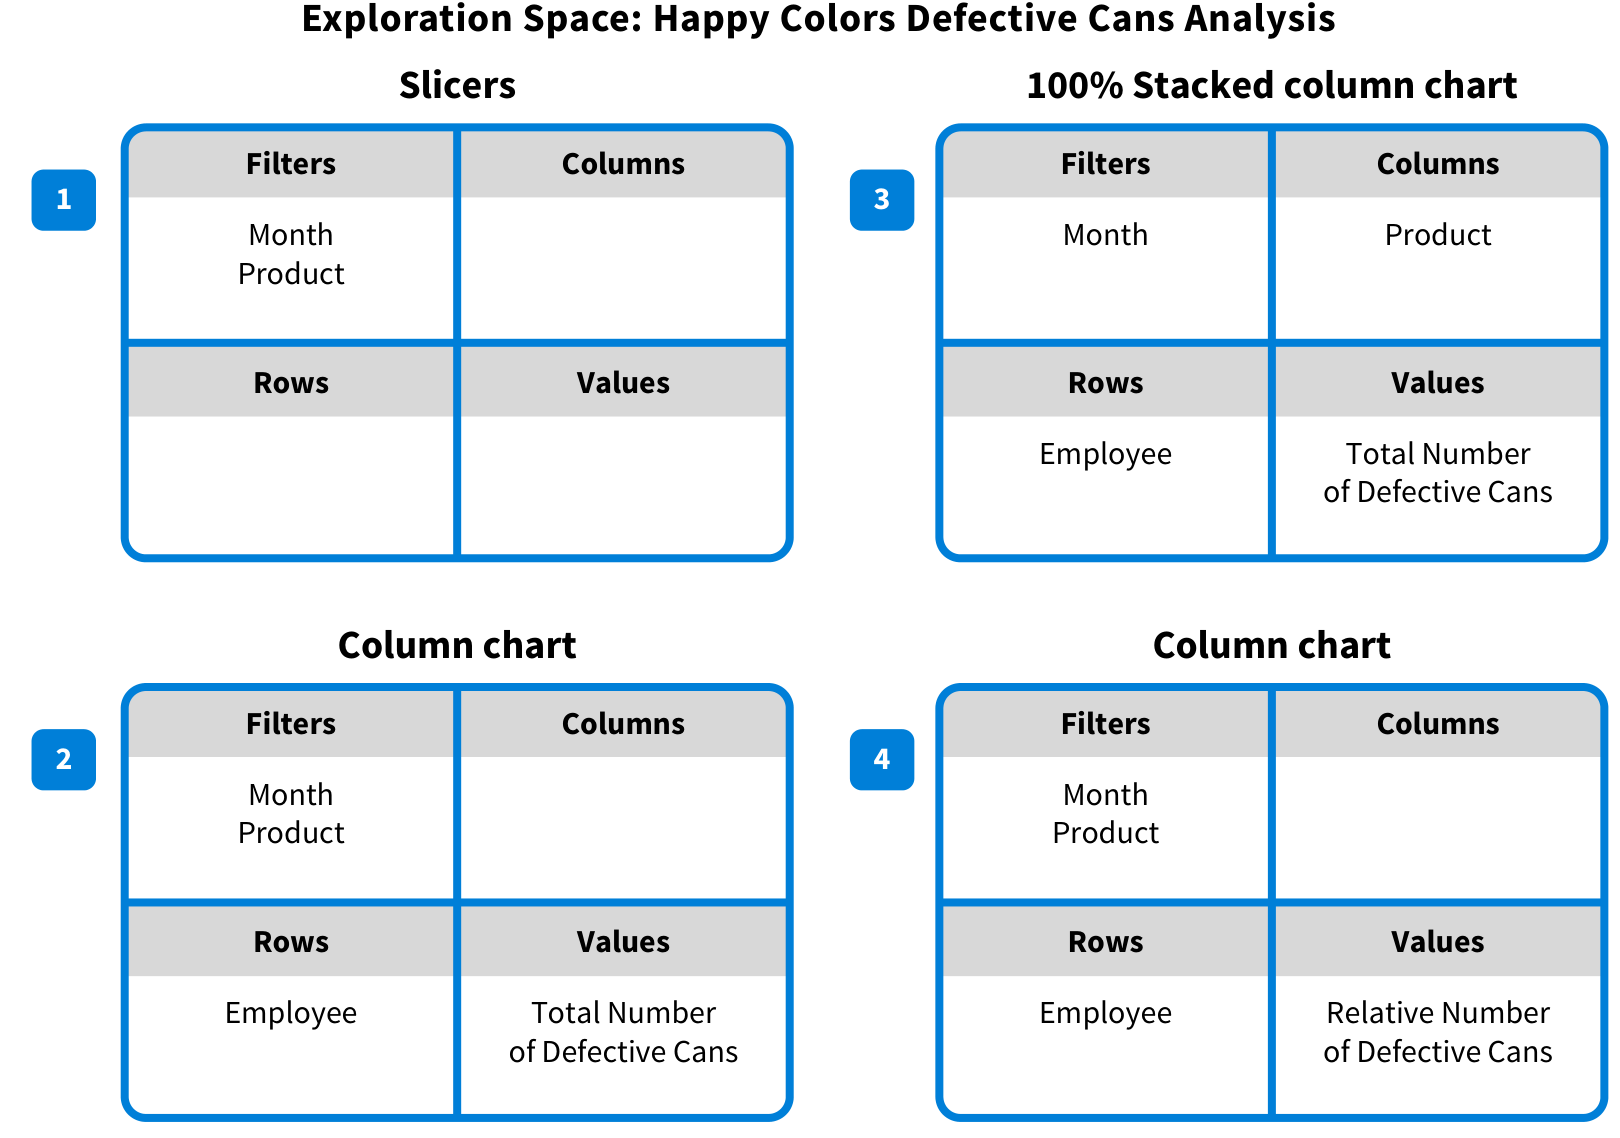
\includegraphics[width=0.95\textwidth,height=0.75\textheight,keepaspectratio]{../textbookForPractice/Figures/Ch_07/Apply It 7.3B.png}
    \end{figure}
\end{frame}

\begin{frame}{Apply It 7.3A\_1}

    \begin{figure}[h]
        \centering
        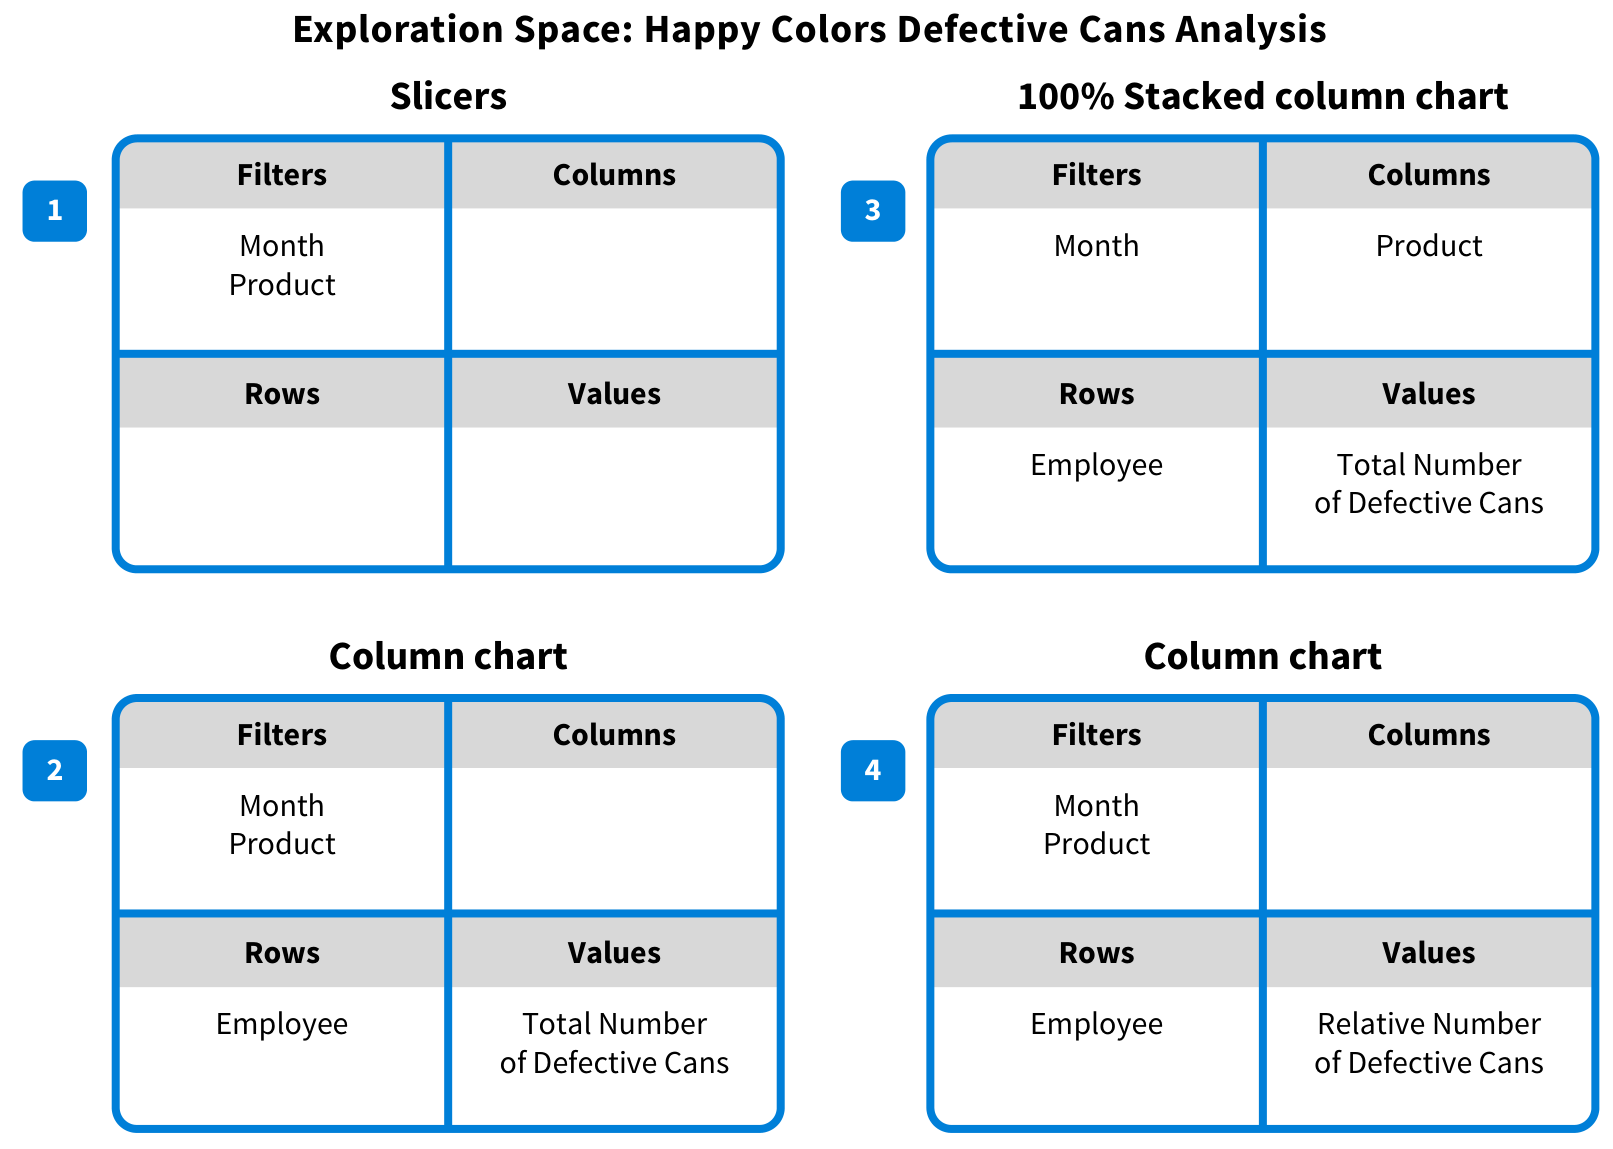
\includegraphics[width=0.95\textwidth,height=0.75\textheight,keepaspectratio]{../textbookForPractice/Figures/Ch_07/Apply It 7.3A_1.png}
    \end{figure}
\end{frame}

\begin{frame}{Apply It 7.3A\_2}

    \begin{figure}[h]
        \centering
        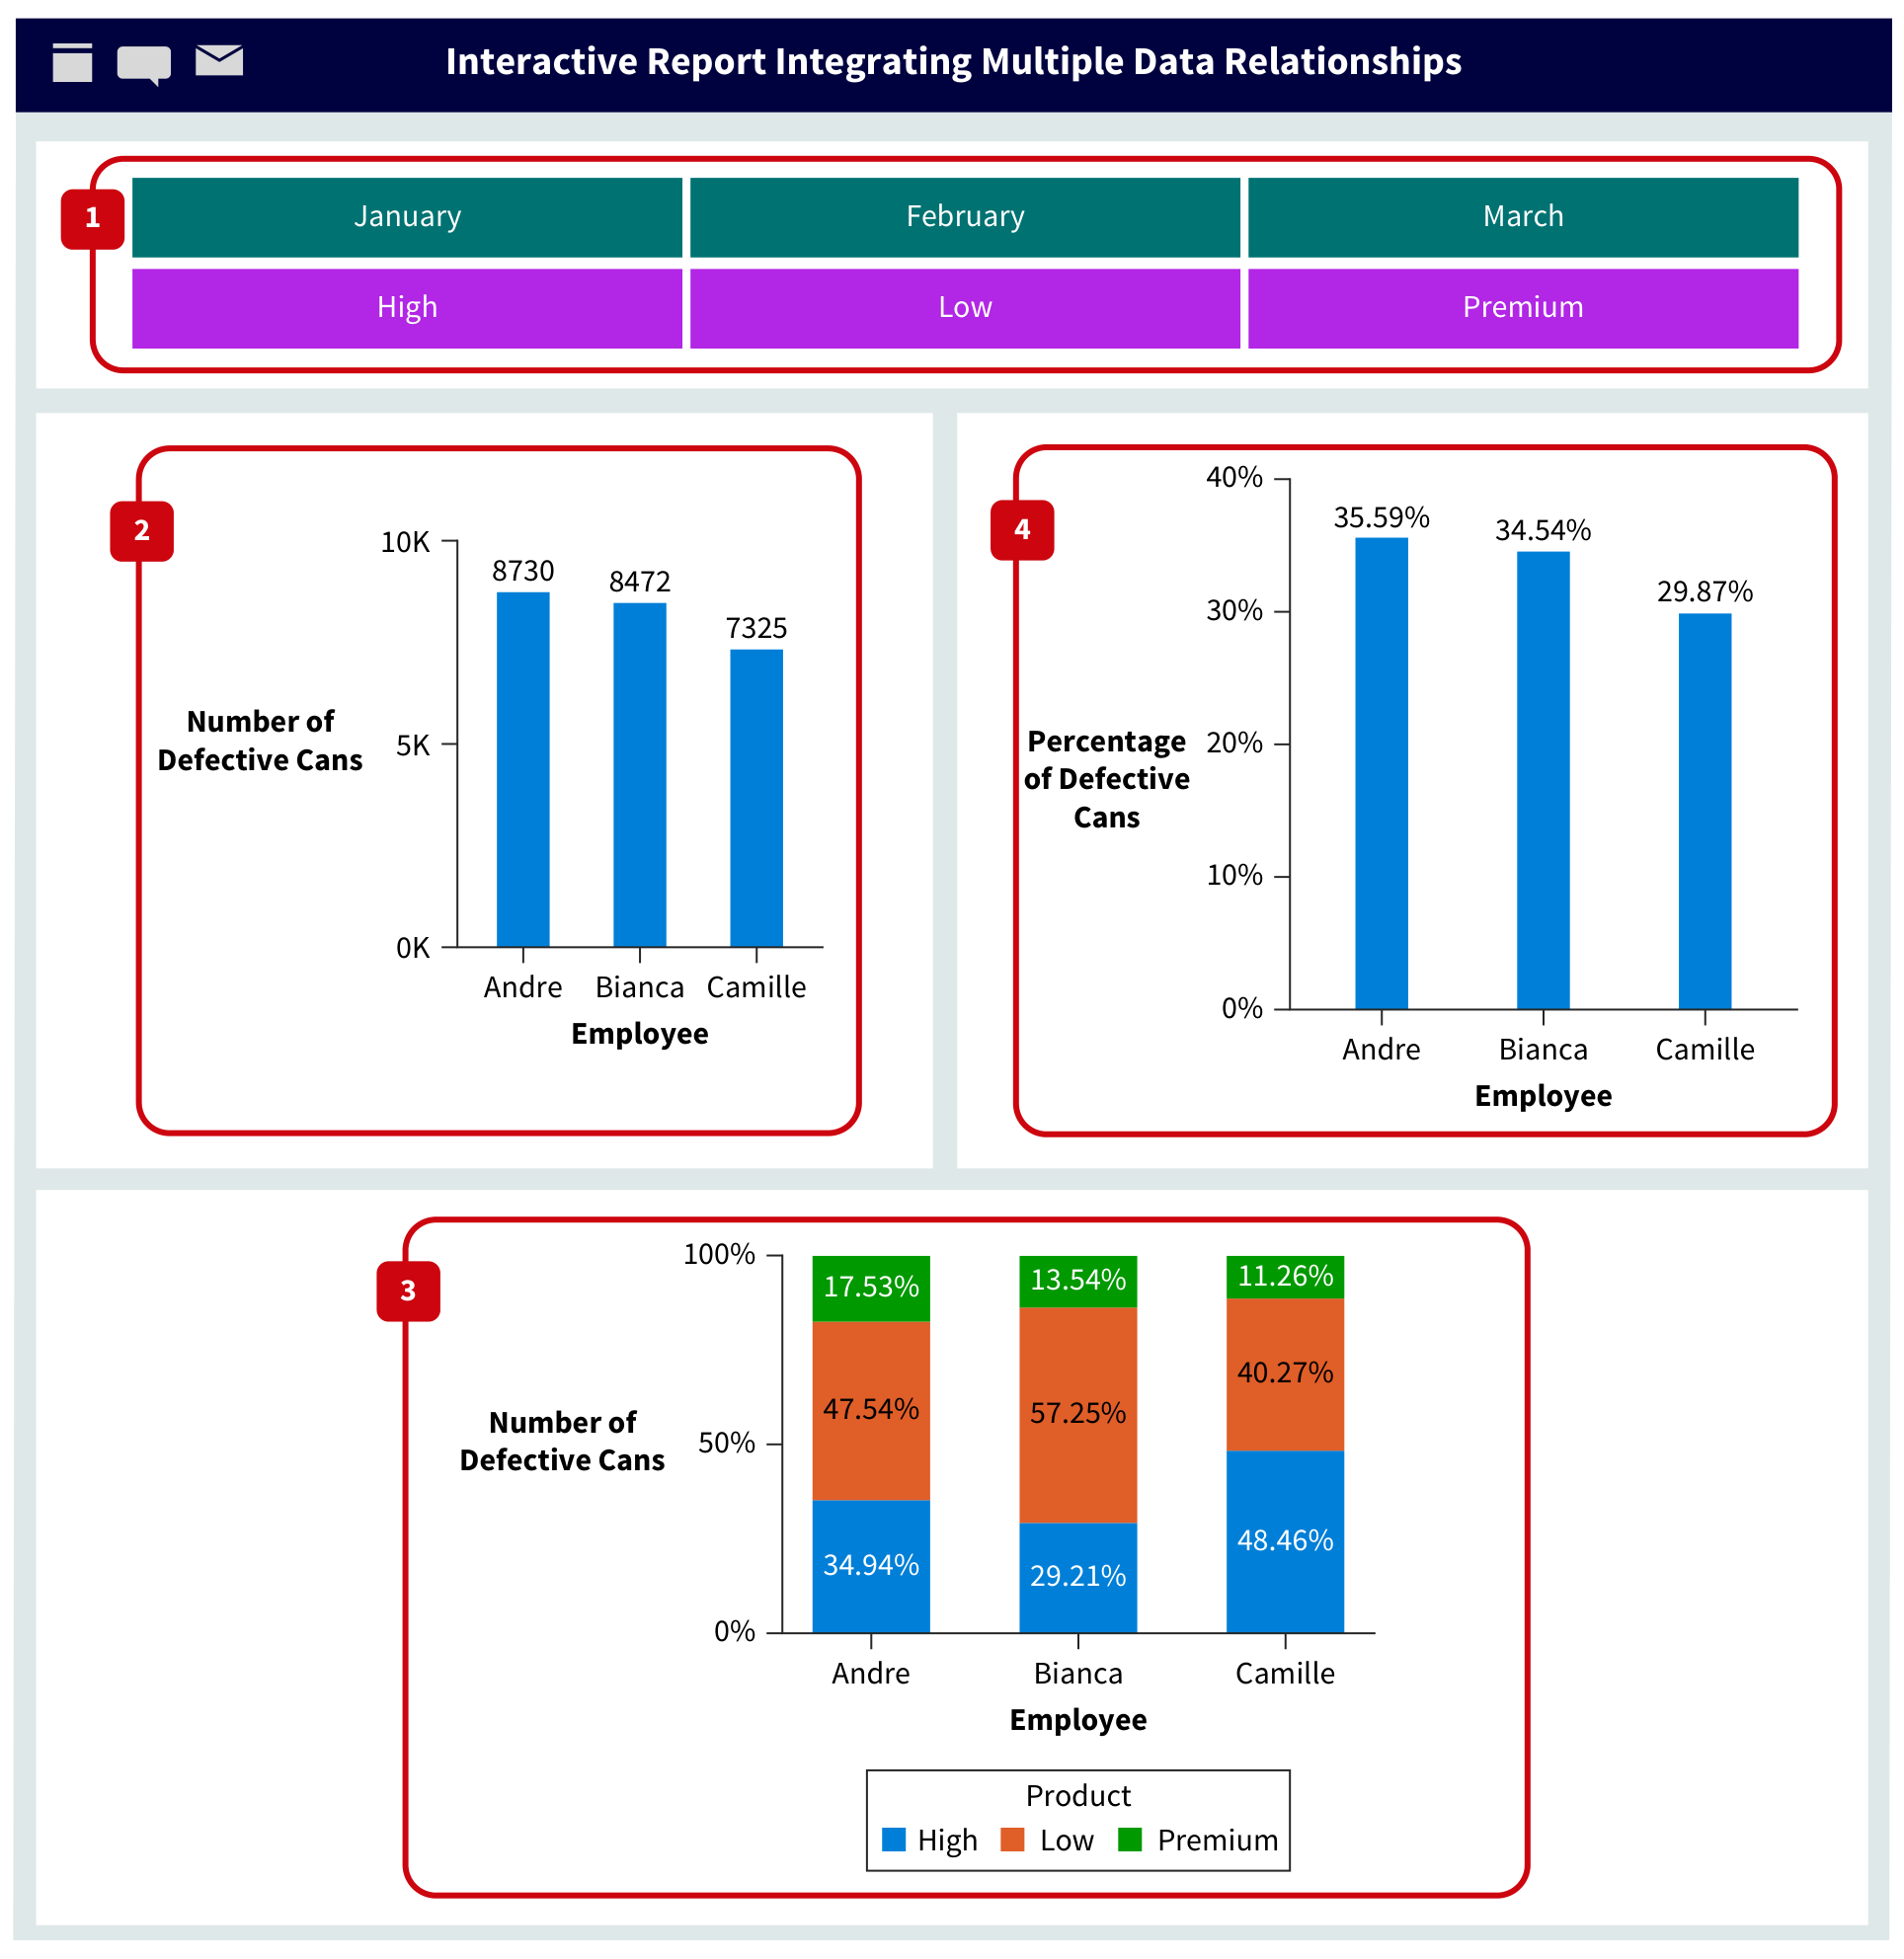
\includegraphics[width=0.95\textwidth,height=0.75\textheight,keepaspectratio]{../textbookForPractice/Figures/Ch_07/Apply It 7.3A_2.png}
    \end{figure}
\end{frame}

\begin{frame}{NoTable 7.16}

    \begin{figure}[h]
        \centering
        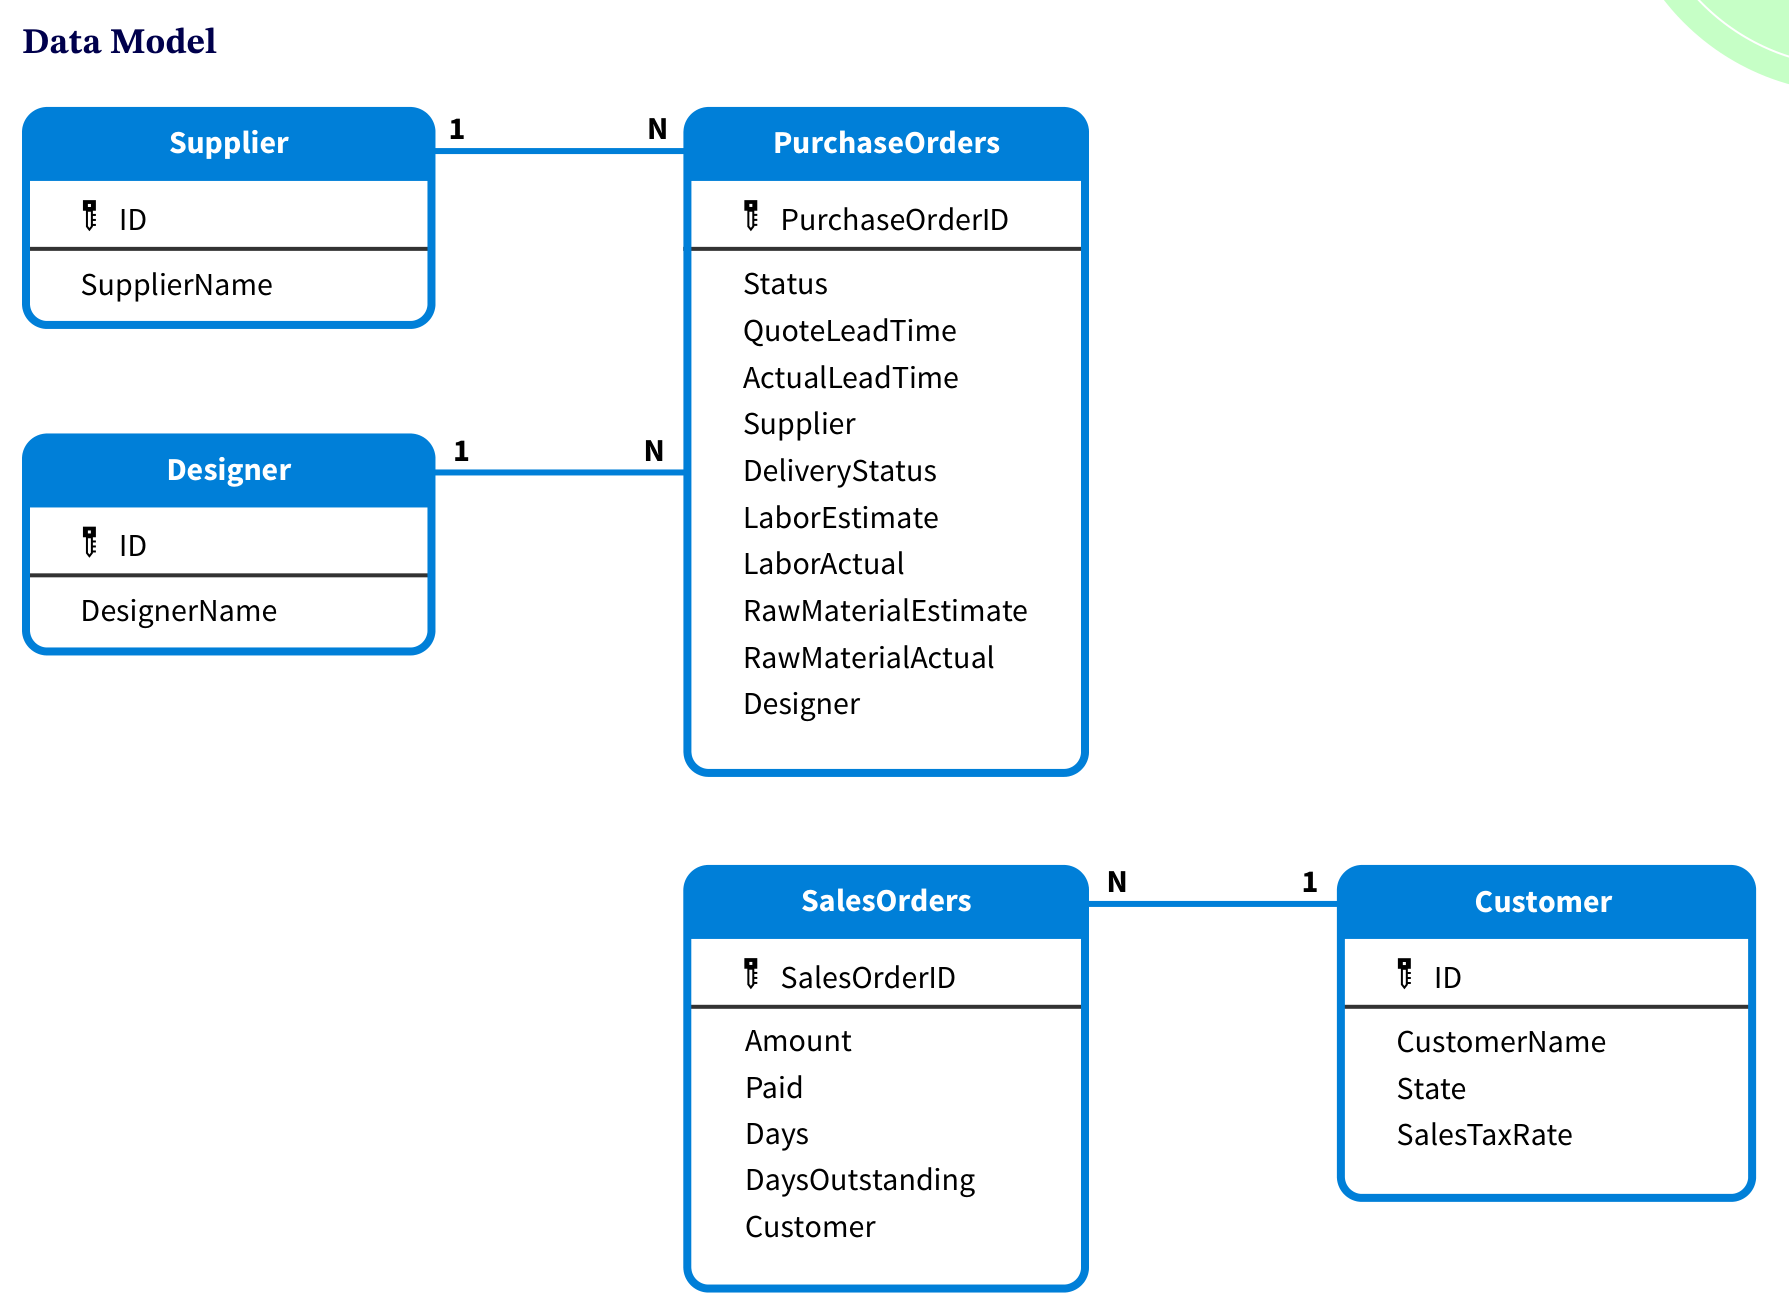
\includegraphics[width=0.95\textwidth,height=0.75\textheight,keepaspectratio]{../textbookForPractice/Figures/Ch_07/NoTable 7.16.png}
    \end{figure}
\end{frame}

\begin{frame}{Kết thúc}
    \begin{center}
        \Huge \textbf{Hỏi \& Đáp} \\
        \vspace{1cm}
        \Large Cảm ơn các bạn đã lắng nghe!
    \end{center}
\end{frame}

\end{document}
